\documentclass[tikz]{article}

% Packages
\usepackage[utf8]{inputenc} % Core latex bundle 
\usepackage[a4paper, total={6in, 9in}]{geometry} % Customize document dimensions and formats
\usepackage{changepage} % Customize page layout in middle of document
\usepackage[table]{xcolor} % Add color to tables
\usepackage{standalone} % Add figures and tables from other files
\usepackage{import} % Import glossary
\usepackage{graphics} % General color and formats
\usepackage{url} % URL formatting
\usepackage{breakurl} % URL formatting
\usepackage{enumitem} % Format list spacing 
\usepackage[hang]{footmisc} % Footnote margins
\usepackage{hyperref} % References
\usepackage{mathtools} % Useful tools for mathematical typesetting and replaces amsmath
\usepackage{amssymb,bm} % Math symbols
\usepackage{svg} % SVG
\usepackage{tikz} % Making charts
\usepackage{array,boldline,multirow,float,booktabs} % Added to make tables
\usepackage{stackengine} % Customize row heights
\usepackage{hhline} % Add double lines to table
\usepackage{multicol} % Two column lists
\usepackage{nicematrix} % Put table lines after color
\usepackage{wrapfig} % Wrap figures in text
\usepackage{tocloft,titletoc} % TOC package
\usepackage{titlesec} % Section spacing
\usepackage{wasysym} % symbols

% Paper formatting
\newlength\LabelWidth
\setlength\parindent{0pt}
\setlength{\parskip}{1em}

% Section spacing
\titlespacing*{\section}
  {0pt}{0.6\baselineskip}{0.6\baselineskip} % Modify section spacing - first \baselineskip is spacing before, second is spacing after the section
\titlespacing*{\subsection}
  {0pt}{0.6\baselineskip}{0.6\baselineskip} % Modify subsection spacing 
\titlespacing*{\subsubsection}
  {0pt}{0.6\baselineskip}{0.6\baselineskip} % Modify subsubsection spacing

% String formats
\newcommand{\code}[1]{\texttt{#1}}
\newcommand{\term}[1]{\textsl{#1}}

% Paper margins
\def\changemargin#1#2{\list{}{\rightmargin#2\leftmargin#1}\item[]}
\let\endchangemargin=\endlist

% Table of contents
\renewcommand{\contentsname}{Table of Contents}
\renewcommand{\cfttoctitlefont}{\Large\bfseries} % TOC title size
\renewcommand{\cftsecleader}{\cftdotfill{\cftdotsep}} % Add dots in TOC to sections
\renewcommand{\cftsecpagefont}{} % Remove \bfseries from section titles' page in TOC

% Section
\renewcommand*{\cftsecnumwidth}{2em} % Increase space section from numbers on left
% \setlength{\cftbeforesecskip}{3pt} % Messes with section TOC length

% Subsection
\cftsetindents{subsection}{1em}{3em} % space between numbers and toc subsections
\setlength{\cftsubsecindent}{2.5em} % subsection number spacing from left
\setlength{\cftbeforesubsecskip}{3pt} % Messes with subsection TOC length was 3pt

% Subsubsection
\cftsetindents{subsubsection}{1em}{4em} % space between numbers and toc subsubsections
\setlength{\cftsubsubsecindent}{5.5em} % subsubsection number spacing from leftindent
\setlength{\cftbeforesubsubsecskip}{3pt} % Messes with subsubsection TOC length was 3pt

% paragraph section
\setcounter{secnumdepth}{4}
\setcounter{tocdepth}{4}

\cftsetindents{paragraph}{1em}{5em} % space between numbers and toc paragraph
\setlength{\cftparaindent}{9.5em} % paragraph number spacing from leftindent
\setlength{\cftbeforeparaskip}{3pt} % Messes with paragraph TOC length was 3pt

% indent after paragraph section
\titleformat{\paragraph}
{\normalfont\normalsize\bfseries}{\theparagraph}{1em}{}
\titlespacing*{\paragraph}
{0pt}{3.25ex plus 1ex minus .2ex}{1.5ex plus .2ex}


% Abstract
% Make abstract justified
\makeatletter
\newcommand{\justified}{
  \rightskip\z@skip
  \leftskip\z@skip}
\makeatother

% Format and size abstract
\makeatletter
\renewenvironment{abstract}{
    \if@twocolumn
      \section*{\abstractname}
    \else 
      \begin{center}
        {\bfseries \large\abstractname\vspace{\z@}} % Bolds abstract name
      \end{center}
      \quotation
    \fi}
    {\if@twocolumn\else\endquotation\fi}
\makeatother

% Delimiters
\DeclarePairedDelimiter\floor{\lfloor}{\rfloor} % Define paired delimiter for floor function
\DeclarePairedDelimiter{\ceil}{\lceil}{\rceil} % Define paired delimiter for ceiling function

% Hyperlinks
\hypersetup{
    colorlinks=true,
    linkcolor=black,
    filecolor=blue,
    urlcolor=black,
}
\urlstyle{same}

% Footnotes
\newcommand{\fref}[1]{\footnote{\href{http://#1}{#1}}}
\setlength{\footnotemargin}{8mm} % Spacing between footnote number and body

% Include tables
\makeatletter
\newcommand{\includetable}[1]{%
  \@ifundefined{tablepath}{%
    \InputIfFileExists{#1}{}{}%
  }{%
    \InputIfFileExists{\tablepath/#1}{}{\InputIfFileExists{#1}{}{}}%
  }
}
\makeatother  

% Table formatting commands
\newcolumntype{Q}{ >{\centering\arraybackslash} m{2.4cm} } % (Figure 5 and 11 - col width)
\newcolumntype{S}{ >{\centering\arraybackslash} m{5.27cm} } % (Figure 12 - col width double)
\newcommand\xrowht[2][0]{\addstackgap[.5\dimexpr#2\relax]{\vphantom{#1}}} % Set row height for tables
\newcommand{\rowh}[1]{\xrowht{40pt}} % Command to set row height for cell with 3 rows
\newcommand{\rowm}[1]{\xrowht{26.667pt}} % Command to set row height for cell with 2 rows
\newcommand{\rows}[1]{\xrowht{13.333pt}} % Command to set row height for cell with 1 rows

% Bean symbols
\newcommand{\BeanCover}{\includesvg[scale=2.2]{./logos/black-bean.svg}} % Logo on cover page
\newcommand{\Bean}{\includesvg[scale=0.23]{./logos/bean.svg}} % Bean used throughout the paper in text form
\newcommand{\bean}{\includesvg[scale=0.17]{./logos/microbean-wide.svg}} % Bean used in formulas - micro bean wide
\newcommand{\tinybean}{\includesvg[scale=0.13]{./logos/microbean-wide.svg}} % Bean used in formulas - micro bean wide
\newcommand{\lambdabean}{\includesvg[scale=0.17]{./logos/microbean.svg}} % Bean used in formulas for lambda superscript - micro bean

% List Key
\SetEnumitemKey{midsep}{topsep=0pt, itemsep=3pt} % Itemize key

% File paths
\newcommand{\tablepath}{figures} % Tables file path
\graphicspath{{figures/}} % Figures file path

%%%%%%%   Begin Document   %%%%%%%
\begin{document}
\pagenumbering{arabic} % Start page numbering style
\thispagestyle{empty} % Hide page numbering
\begin{titlepage}
    \begin{center}
        \vspace*{-0.1cm}
        \begin{changemargin}{-0.25cm}{-0.25cm}
        \centering % added to center title
        \textbf{\Large{Beanstalk: A Permissionless Fiat Stablecoin Protocol}}
        \end{changemargin}
        \begin{center}
        \BeanCover
        \end{center}
        
        \vspace{0.4cm}
        \begin{center}
        \begin{tabular}{>{\centering\arraybackslash}p{6cm} >{\centering\arraybackslash}p{6cm}}
                \large{Publius} & \large{Beanstalk Farms} \\
                \href{mailto:beanstalk.publius@protonmail.com}{\normalsize{beanstalk.publius@protonmail.com}} & \href{mailto:beanstalkfarms@protonmail.com}{\normalsize{beanstalkfarms@protonmail.com}}
            \end{tabular}
        \end{center}
        % \vspace{0.4cm}
        % \large{Publius, Beanstalk Farms}
            
        % \vspace{-0.25cm}
        % \normalsize{beanstalk.publius@protonmail.com, beanstalkfarms@protonmail.com}
        
        \vspace{-0.25cm}
        \normalsize{\href{https://bean.money/}{bean.money}}
        
        \vspace{0.4cm}
        \footnotesize{Published:} \normalsize{August 6, 2021}
        
        \vspace{-0.25cm}
        \footnotesize{Modified:} \normalsize{October 16, 2023}
        
        \vspace{-0.25cm}
        \footnotesize{Whitepaper Version:} {\normalsize{2.6.0}}
        
        \vspace{-0.25cm}
        \footnotesize{Code Version:} \href{https://github.com/BeanstalkFarms/Beanstalk}{\normalsize{2.6.0}}\footnote{\href{https://github.com/BeanstalkFarms/Beanstalk}{github.com/BeanstalkFarms/Beanstalk}}
        

        \vspace{0.1cm}
        \flushleft{\normalsize{\term{“A national debt if it is not excessive will be to us a national blessing; it will be powerfull cement of our union.”}}}
    
        \normalsize{\hspace{2.5em}- Alexander Hamilton, Letter to Robert Morris, April 30, 1781}\fref{founders.archives.gov/documents/Hamilton/01-02-02-1167}
        \vspace{0.4cm}
        \begin{abstract}
            \justified{\normalsize{\noindent Financial applications built on decentralized, permissionless computer networks, collectively referred to as decentralized finance (DeFi), often require a “stablecoin”: a network-native asset with sufficiently low volatility in value relative to an arbitrary value peg (\term{e.g.}, 1 US Dollar (USD, \$), 100 Satoshis and 1 oz of Gold). To date, flawed stablecoin implementations sacrifice the main benefits of trustless computing by requiring a custodian or limit their potential supply and utility by imposing collateral requirements, and suffer from noncompetitive carrying costs. A stablecoin that does not compromise on decentralization nor require collateral, has competitive carrying costs, and trends toward more stability and liquidity, will unlock the potential of DeFi. We propose an Ethereum\fref{ethereum.org}-native, fiat stablecoin protocol that issues an ERC-20 Standard\fref{ethereum.org/en/developers/docs/standards/tokens/erc-20} token that fulfills these requirements. A decentralized autonomous organization (DAO) governed by a variable supply, yield generating token simultaneously provides security, dampens price volatility and encourages consistent liquidity growth. Beanstalk uses a decentralized credit facility, network-native price oracle, variable supply and self-adjusting interest rate, to regularly cross the stablecoin price over its value peg without requiring action from users.}}
        \end{abstract}
   \end{center}
\end{titlepage}

\newpage

% TOC formatting
% \addtocontents{toc}{\protect\enlargethispage{20mm}} % TOC margins
\thispagestyle{empty} % Hide TOC page numbering 
\addtocontents{toc}{\protect\thispagestyle{empty}} % Allow hiding both TOC page numbers

\cleardoublepage
\pagenumbering{gobble}
{\large\tableofcontents} % Compile TOC with large font
\cleardoublepage
\pagenumbering{arabic}

% \thispagestyle{empty} % Hide TOC page numbering
% \addtocontents{toc}{\protect\thispagestyle{empty}} % Allow hiding both TOC page numbers

\newpage
\setcounter{page}{5} % Begin page numbering

\section{Introduction}
Decentralized computer networks that run on open source, permissionless protocols (\term{e.g.}, Bitcoin\fref{bitcoin.org} and Ethereum) present the next economic and technological frontiers: trustless goods and services. Instead of requiring users to trust (1) a rent-seeking third party to write secure code, run it on secure computer servers and perform fair system administration, or (2) concentrated risk-taking counterparties, trustless technology brings control back to users. Anyone can verify the security, authenticity and policies of open source software for themselves. Any computer with an internet connection can use and participate in maintenance of permissionless networks. Protocol-native financial incentives encourage participation in network maintenance. Diverse sets of users and network maintenance participants remove concentrated counterparty risk, which creates decentralization. The combination of permissionlessness, sound economics and decentralization creates censorship resistance, which is fundamental to trustlessness. Potential applications built on top of well designed trustless networks are infinite.

A key promise of trustless computer networks is the widespread use of financial goods and services without the need for trust-providing, rent-seeking central authorities, or concentrated counterparties. However, as blockchains that support trustless networks are adopted, the values of their native assets (\term{e.g.}, Bitcoin and Ether (ETH)) change radically. To date, the practicality of using DeFi technologies for real economic activity is limited by the lack of a trustless network-native asset with competitive carrying costs, low-volatility endogenous value and deep liquidity.

A stablecoin protocol generates a fungible network-native asset and attempts to keep its price volatility sufficiently low relative to an arbitrary value peg. Stablecoin utility is a function of trustlessness, carrying costs, stability and liquidity. A stablecoin's trustlessness, carrying costs, stability and liquidity are primarily functions of the source of its value. Current implementations fail to deliver a stablecoin that is (1) sufficiently decentralized and permissionless, (2) unrestricted by collateral requirements and their associated noncompetitive carrying costs, (3) sufficiently low in price volatility relative to its value peg and (4) highly liquid, due to a lack of endogenous value creation.

\subsection{Convertible Stablecoins}
Non-network-native exogenous value convertible stablecoin protocols (\term{e.g.}, US Dollar Coin\fref{circle.com/usdc} (USDC), Tether\fref{tether.to} (USDT), Wrapped Bitcoin,\fref{wbtc.network} and RenBTC\fref{renproject.io}) issue stablecoins they claim are collateralized by, and require a custodian that facilitates the convertibility to, non-network-native exogenous value worth at least 100\% of total outstanding protocol liabilities. Stablecoin protocols that offer convertibility to non-network-native assets function as low-volatility permissioned bridges between their respective networks and the rest of the world. Arbitrage opportunities created by convertibility ensure the price of the network-native asset is rarely above or below the value of the custodied value when accounting for frictions around conversions. However, users of non-network-native exogenous value convertible stablecoins sacrifice permissionlessness and carry entirely: third parties custody the non-network-native assets, can freeze the network-native assets unilaterally and can retain yield earned on collateral. The absence of protocol-native opportunities for carry limits liquidity.

\newpage
Network-native exogenous value convertible stablecoin protocols (\term{e.g.}, Maker\fref{makerdao.com} (DAI) and Abracadabra\fref{abracadabra.money}) use excess network-native collateral to remove most points of centralization. Overcollateralization removes most risk associated with the volatility of the collateral but by necessity requires the introduction of rent payments in order to prevent the value of the stablecoin from trending towards the value of the underlying collateral. The combination of collateral requirements and rent payments significantly limits the potential supply of these stablecoins. Liquity\fref{liquity.org} is an ideal simple iteration of a network-native exogenous value convertible stablecoin protocol, without any points of centralization and with protocol-native positive carry. In order to remove rent payments, Liquity does not target an exact price for its stablecoin, LUSD. The potential supply of LUSD is limited by the value of trustless network-native value. 

Despite the shortcomings of exogenous value convertible stablecoin implementations, demand for their USD implementations continues to increase rapidly. Over the twelve months prior to the initial deployment of Beanstalk, the total market capitalization of exogenous value convertible USD stablecoins increased more than 500\% to over \$100 Billion.\fref{stablecoinindex.com/marketcap} However, despite this rapid increase in supply, the borrowing rates on exogenous value convertible USD stablecoins have historically been higher\fref{app.aave.com/markets} than borrowing rates on USD.\fref{newyorkfed.org/markets/reference-rates/effr} Noncompetitive carrying costs are due to collateral requirements. Businesses built on trustless primitives cannot compete with businesses built on centralized systems due to noncompetitive carrying costs on low-volatility network-native trustless assets.

To date, implementations of purely endogenous value convertible stablecoins (\term{e.g.}, Terra\fref{allcryptowhitepapers.com/terra-whitepaper}) have failed. While hybrid value convertible stablecoins (\term{e.g.}, FRAX\fref{frax.finance}) have demonstrated some efficacy at peg maintenance at high proportions of exogenous value, their supply is limited by network-native exogenous value. 

\vspace*{-1.5mm}
\subsection{Non-convertible Stablecoins}
\vspace*{-1.5mm}
Non-convertible stablecoin protocols adjust themselves mechanically to return the price of their stablecoin to their value peg without convertibility to collateral. It is impossible to keep a stablecoin price equal to its value peg without low-friction convertibility. Non-convertible stablecoin protocols without collateral requirements have the potential to create endogenous value that facilitates trustlessness, competitive carrying costs and deep liquidity at the expense of volatility. 

Rebasing stablecoin protocols (\term{e.g.}, Ampleforth\fref{ampleforth.org}) have shown efficacy at crossing their stablecoin prices over their value pegs, but without the regularity, low volatility or liquidity necessary to create utility. Extreme negative carrying costs during decreases in demand exacerbate difficulty of use.

The value of fiat currency is derived from the credit of its issuer and its utility. Utility of fiat currency is a function of trustlessness, carrying costs, stability and liquidity. Decentralized credit can be used to issue a permissionless fiat stablecoin with competitive carrying costs, low volatility and deep liquidity.

To date, however, implementations of fiat stablecoin protocols have failed to regularly cross their stablecoin prices over their value pegs with sufficiently low volatility due to poorly designed peg maintenance mechanisms or seigniorage models that disproportionately reward speculators at the expense of stablecoin utility. 

\subsection{Beanstalk}
Beanstalk uses a dynamic peg maintenance mechanism to regularly cross the price of 1 Bean (\Bean) \textbf{--} the Beanstalk ERC-20 Standard fiat stablecoin \textbf{--} over its value peg without centralization or collateral requirements. Instead of holding a perfect peg, Beanstalk creates user confidence by consistently crossing the price of \Bean1 over its value peg with increased frequency and decreased volatility over time. Regularly crossing the price of \Bean1 over its value peg creates the opportunity to regularly buy and sell Beans at their value peg.

Beanstalk consists of five interconnected components: (1) a decentralized timekeeping and execution facility, (2) a decentralized governance facility, (3) a decentralized credit facility, (4) a decentralized exchange (DEX), and (5) an interface to interact with other Ethereum-native protocols via Beanstalk. Beanstalk-native financial incentives are used to coordinate the components to (1) create a stablecoin with competitive carrying costs, (2) regularly cross the price of \Bean1 over its value peg during both long run decreases and increases in demand for Beans, and (3) attract deep liquidity, in a cost-efficient, permissionless and decentralized fashion.

Beanstalk is designed from economic first principles to create a useful trustless fiat currency. Over time, trustlessness, stability and liquidity increase, while carrying costs decrease but remain competitive. The following principles inspire Beanstalk:
\begin{itemize}[midsep]
    \item Low concentration of ownership;
    \item Strong credit;
    \item The marginal rate of substitution;
    \item Low friction;
    \item Equilibrium; and
    \item Incentive structures determine behaviors of financially motivated actors.
\end{itemize}

\section{Previous Work}
Beanstalk is the culmination of previous development, evolution and experimentation within the DeFi ecosystem. 

A robust, trustless computer network that supports composability and fungible token standards (\term{e.g.}, Ethereum) with a network-native automated market maker (AMM) decentralized exchange (\term{e.g.}, Uniswap\fref{uniswap.org} and Curve\fref{curve.fi}) is required to implement a decentralized stablecoin. 

Stablecoin protocols that offer convertibility to the non-network-native asset they are pegged to reliably bridge the value of non-network-native assets to the network. Beanstalk leverages the existence of non-network-native exogenous value convertible stablecoins that trade on AMMs to create a new permissionless stablecoin with a non-network-native value peg.

Beanstalk was inspired by Empty Set Dollar.\fref{emptyset.finance} The failures of Empty Set Dollar and similar stablecoin implementations provided invaluable information that influenced the design of Beanstalk.

\section{Farm}
Well designed decentralized protocols create utility for end users without requiring, but never limiting, participation in protocol maintenance. Protocol-native financial incentives encourage performance of work to create utility for end users. Low barriers to and variety in work enable a diverse set of participants. A diverse set of well incentivized workers can create censorship resistant utility. 

Beanstalk does not require actions from, impose rent on, or affect in any way, regular Bean users (\term{e.g.}, smart contracts). Anyone can join the \term{Farm} to use Beanstalk and profit from participation in protocol maintenance. Governance of Beanstalk upgrades, Bean peg maintenance and use of Beans take place on the \term{Farm}.

The \term{Farm} has five primary components: the \term{Sun}, \term{Silo}, \term{Field}, \term{Market} and \term{Depot}. Beanstalk-native financial incentives coordinate the components to create a stalwart system of governance, regularly cross the price of \Bean1 over its value peg, consistently grow Bean liquidity and maximize composability, without collateral.

The \term{Sun} offers payment for participation in timekeeping and execution. Time on the \term{Farm} is kept in \term{Seasons}. Anyone can earn Beans for successfully calling the \code{gm} function to begin the next \term{Season} at the top of each hour.

The \term{Silo} is the Beanstalk DAO. The \term{Silo} offers passive yield opportunities to owners of \Bean\ and other assets (\hyperlink{ht126}{$\lambda$}) on the \term{Deposit Whitelist} (\hyperlink{ht127}{$\Lambda$}) (\term{i.e.}, $\Bean \subset \lambda \in \Lambda$) for participation in governance of Beanstalk upgrades and passive contribution to security, stability and liquidity. Anyone can become a \term{Stalkholder} by \term{Depositing} \hyperlink{ht126}{$\lambda$} into the \term{Silo} to earn \term{Stalk}. \term{Stalkholders} govern Beanstalk upgrades and are rewarded with Beans when the Bean supply increases. Active contributions to peg maintenance within the \term{Silo} earn additional \term{Stalk}.

The \term{Field} offers yield opportunities to \term{Sowers} (creditors) for participation in peg maintenance. Anyone can become a \term{Sower} by lending Beans that are not in the \term{Silo} to Beanstalk. Bean loans are repaid to \term{Sowers} with interest when the Bean supply increases. 

The \term{Market} offers 0-fee trading to anyone using the Ethereum network.

The \term{Depot} facilitates interactions with other Ethereum-native protocols through Beanstalk in a single transaction.

\section{Sun}
The Beanstalk governance and peg maintenance mechanisms require a protocol-native timekeeping mechanism and regular code execution on the Ethereum blockchain. The \term{Sun} creates a cost-efficient protocol-native timekeeping mechanism and incentivizes cost-efficient code execution on Ethereum at regular intervals. In general, Beanstalk uses Ethereum block timestamps (\hyperlink{ht69}{$E$}), such that $\hyperlink{ht69}{E} \in \mathbb{Z}^{+}$.

We define a \term{Season} (\hyperlink{ht204}{$t$}), such that $\hyperlink{ht204}{t} \in \mathbb{Z}^{+}$, as an approximately 3,600 second (1 Hour) interval. The first \term{Season} begins when a successful transaction on the Ethereum blockchain that includes a \code{gm} function call is committed. When Beanstalk accepts the \code{gm} function call, the necessary code is executed.

Beanstalk only accepts one \code{gm} function call per \term{Season}. Beanstalk accepts the first \code{gm} function call provided that the timestamp in the Ethereum block containing it is sufficiently distant from the timestamp in the Ethereum block containing the Beanstalk deployment (\hyperlink{ht70}{$E_1$}).

The minimum timestamp Beanstalk accepts a \code{gm} function call for a given \hyperlink{ht204}{$t$} (\hyperlink{ht75}{$E_{t}^{\text{min}}$}), $\forall\ \hyperlink{ht75}{E_{t}^{\text{min}}}$ such that $1 < \hyperlink{ht204}{t}$, and \hyperlink{ht70}{$E_1$} is:
$$\hyperlink{ht75}{E_{t}^{\text{min}}} = 3600{\left({\left\lfloor\frac{\hyperlink{ht70}{E_1}}{3600}\right\rfloor} + \hyperlink{ht204}{t}\right)}$$

The cost to execute the \code{gm} function changes depending on the traffic on the Ethereum network and the state of Beanstalk. Beanstalk covers the transaction cost by awarding the sender of an accepted \code{gm} function call with newly minted Beans. 

To encourage regular \code{gm} function calls even during periods of congestion on the Ethereum network while minimizing cost, the award for successfully calling the \code{gm} function for $t$ ($a_t$) is based on (1) an approximation of the cost to call the \code{gm} function in Beans in the current block ($\sun_{\Xi}$), (2) the inter-block maximum extractable value (MEV) manipulation resistant time weighted average (TWA) Bean reserves in the Multi Flow \term{Pump}\fref{basin.exchange/multi-flow-pump.pdf}$^{,}$\fref{etherscan.io/address/0xBA510f10E3095B83a0F33aa9ad2544E22570a87C} of the BEAN:ETH \term{Well}\fref{basin.exchange/basin.pdf}$^{,}$\footnote{Any italicized terms not defined herein are defined by Basin.} from the beginning of the \term{Season} to the current transaction ($\Theta^{\text{SMA}}_{\bean,t_0,\Game}$), and (3) the minimum number of Beans that must be in the BEAN:ETH \term{Well} in order for the oracle to be considered ($\Theta^{\text{min}(\bean)}$), such that $a_t,\ \sun_{\Xi},\ \Theta^{\text{SMA}}_{\bean,t_0,\Game},\ \Theta^{\text{min}(\bean)} \in \{j \times 10^{-6} \mid j \in \mathbb{Z}^{+} \}$, and compounds 1\% every additional second that elapses past $E_t^{\text{min}}$ for 300 seconds. 

$\sun_{\Xi}$ is based on approximations of (1) the gas used to execute the \code{gm} function call ($\varrho$), (2) the gas fee of the current block denominated in Wei ($\varpi_\Xi$), such that $\varrho,\ \varpi_\Xi \in \mathbb{Z}^{+}$, and (3) the current price of ETH in Beans ($\vartheta$), such that $\vartheta \in \{j \times 10^{-6} \mid j \in \mathbb{Z}^{+} \}$, up to a maximum of 100 Beans.

Beanstalk calculates $\varrho$ as the difference between \code{gasleft}\fref{docs.soliditylang.org/en/v0.7.6/units-and-global-variables.html\#block-and-transaction-properties} at the beginning and end of the \code{gm} function call ($\varsigma$), such that $\varsigma \in \mathbb{Z}^{+}$, up to a maximum of $5 \times 10^5$ gas:

$$\varrho = \text{min}(\varsigma + 10^5,\ 5 \times 10^5)$$

We define $\varpi_\Xi$ as the result of \code{block.basefee}\fref{docs.soliditylang.org/en/v0.8.7/units-and-global-variables.html\#block-and-transaction-properties} read through a separate contract\fref{etherscan.io/address/0x84292919cB64b590C0131550483707E43Ef223aC\#code} plus a 5 Wei buffer to account for the priority fee:

$$\varpi_\Xi = \code{block.basefee} + 5$$

$\vartheta$ is based on $\Theta^{\text{SMA}}_{\bean,t_0,\Game}$ and the inter-block MEV manipulation resistant TWA ETH reserves in the Multi Flow \term{Pump} of the BEAN:ETH \term{Well} from the beginning of the \term{Season} to the current transaction ($\Theta^{\text{SMA}}_{\text{ETH},t_0,\Game}$), such that $\Theta^{\text{SMA}}_{\text{ETH},t_0,\Game} \in \{j \times 10^{-18} \mid j \in \mathbb{Z}^{+} \}$:
$$ \vartheta = \frac{\Theta^{\text{SMA}}_{\bean,t_0,\Game} \times 10^{18}}{\Theta^{\text{SMA}}_{\text{ETH},t_0,\Game}}$$

Therefore, we define $\sun_{\Xi}$ for a given $\varrho$, $\varpi_\Xi$ and $\vartheta$ as:

$$\sun_{\Xi} = \text{min}(\varrho \times \varpi_\Xi \times \vartheta + 3,\ 100)$$

Therefore, we define $a_t$ for a given $\sun_{\Xi}$, $\Theta^{\text{SMA}}_{\bean,t_0,\Game}$, $\Theta^{\text{min}(\bean)}$, the timestamp of the current block ($E_\Xi$), and $\hyperlink{ht75}{E_{t}^{\text{min}}}$ as:

$$ a_t =
\begin{cases}
{100} & \text{if} \; t = 1 \mkern3mu | \mkern3mu \Theta^{\text{SMA}}_{\bean,t_0,\Game} < \Theta^{\text{min}(\bean)}  \\
{\sun_{\Xi} \times 1.01^{\text{min}\{{\hyperlink{ht74}{E_\Xi} - \hyperlink{ht75}{E_{t}^{\text{min}}}},\ 300\}}} & \text{else}
\end{cases} 
$$

To minimize the cost of calculating \hyperlink{ht11}{$a_t$}, the \term{Sun} uses a binomial estimation with a margin of error of less than 0.05\% of \hyperlink{ht11}{$a_t$}. Thus, Beanstalk creates a cost-efficient protocol-native timekeeping mechanism and ensures cost-efficient code execution on the Ethereum blockchain at regular intervals.

\vspace*{-1mm}
\section{Silo}
\vspace*{-1mm}
Beanstalk requires the ability to coordinate protocol upgrades. The \term{Silo} \textbf{--} the Beanstalk DAO \textbf{--} uses the \term{Stalk System} to create protocol-native financial incentives that coordinate Beanstalk upgrades and consistently improve security, stability and liquidity. \term{Stalkholders} earn passive yield from participation in governance of Beanstalk upgrades and passive contributions to security, stability and liquidity. Active contributions to peg maintenance within the \term{Silo} earn additional \term{Stalk}.

\vspace*{-1.3mm}
\subsection{The Stalk System}
\vspace*{-1.3mm}
The \term{Stalk System} decentralizes ownership over time and creates Beanstalk-native financial incentives to (1) align DAO voters' interests with the health of Beanstalk, (2) leave assets \term{Deposited} in the \term{Silo}, and (3) allocate liquidity in ways that benefit Beanstalk.

Anyone can become a \term{Stalkholder} by \term{Depositing} assets on the \term{Deposit} \term{Whitelist} into the \term{Silo} to earn \term{Stalk} and \term{Seeds}. \term{Stalk} and \term{Seeds} are not liquid. Every \term{Season}, $1 \times 10^{-4}$ additional \term{Stalk} \term{Grows} from each \term{Seed}. \term{Grown} \term{Stalk} become \term{Stalk} when \term{Mown}. \term{Grown} \term{Stalk} from \hyperlink{ht126}{$\lambda$} \term{Deposits} are automatically \term{Mown} each time a \term{Stalkholder} interacts with \hyperlink{ht126}{$\lambda$} in the Silo (\term{i.e.}, \term{Deposit}, \term{Withdraw}, \term{Convert}, \term{Transfer}, \term{Plant} and \term{Enroot}), or when they call the \code{mow} or \code{mowMultiple} function with \hyperlink{ht126}{$\lambda$}.

\term{Stalkholders} are entitled to participate in Beanstalk governance and a portion of Bean mints. The influence in governance of, and distribution of Beans paid to, a \term{Stalkholder} are proportional to their \term{Stalk} holdings relative to total outstanding \term{Stalk}. \term{Stalk} holdings become less concentrated over time.

\vspace*{-1.3mm}
\subsection{Deposit Whitelist}
\vspace*{-1.3mm}
Any ERC-20 Standard token can be added to and removed from \hyperlink{ht127}{$\Lambda$} via Beanstalk governance. \Bean\ is always on the \term{Deposit} \term{Whitelist}.

In order for a given \hyperlink{ht126}{$\lambda$} to be added to \hyperlink{ht127}{$\Lambda$} Beanstalk requires (1) its token address, (2) a function to calculate the flash-loan-resistant Bean-denominated-value (BDV) for a given number of \hyperlink{ht126}{$\lambda$} \term{Deposited}, (\hyperlink{ht84}{$f^{\lambda}(z^{\lambda})$}), such that $z^{\lambda} \in \{j \times 10^{-6} \mid j \in \mathbb{Z}^{+} \}$, $f^{\lambda}\colon \{j \times 10^{-\lambda} \mid j \in \mathbb{Z}^{+} \} \rightarrow \{j \times 10^{-6} \mid j \in \mathbb{Z}^{+} \}$, where $z^{\lambda}$ is the number of \hyperlink{ht126}{$\lambda$} \term{Deposited}, (3) the number of \term{Stalk} per BDV of \hyperlink{ht126}{$\lambda$} \term{Deposited} (\hyperlink{ht120}{$k^{\lambda}$}), such that $\hyperlink{ht120}{k^{\lambda}} \in \{j \times 10^{-4} \mid j \in \mathbb{Z}^{+} \}$, and (4) the number of \term{Seeds} per BDV of \hyperlink{ht126}{$\lambda$} \term{Deposited} (\hyperlink{ht32}{$c^{\lambda}$}), such that $\hyperlink{ht32}{c^{\lambda}} \in \mathbb{Z}^{+}$, to be stored.

\vspace*{-1mm}
\subsection{Deposits, Withdrawals, Transfers and Conversions}
\vspace*{-1mm}
\hyperlink{ht126}{$\lambda$} can be \term{Deposited} into, \term{Withdrawn} from and \term{Converted} within, the \term{Silo} at any time.

\vspace*{-1mm}

Beanstalk rewards \term{Stalk} and \term{Seeds} to \term{Depositors} immediately upon \term{Depositing} \hyperlink{ht126}{$\lambda$} into the \term{Silo} based on its BDV when \term{Deposited}, \hyperlink{ht120}{$k^{\lambda}$} and \hyperlink{ht32}{$c^{\lambda}$}. \term{Deposits} implement the ERC-1155 Standard.\fref{ethereum.org/en/developers/docs/standards/tokens/erc-1155}

Upon a \term{Deposited} asset's \term{Withdrawal} from the \term{Silo}, the \term{Deposit} itself is burned and the number of \term{Stalk}, \term{Seeds}, and \term{Stalk} from \term{Seeds} rewarded to it must also be forfeited. 

The number of \term{Stalk}, \term{Seeds}, and \term{Stalk} from \term{Seeds} rewarded to a \term{Deposit} are included in its \term{Transfer} to another address.

\term{Conversions} of \term{Deposited} \hyperlink{ht126}{$\lambda$} to \term{Deposited} $\lambda'$ are permissioned by a \term{Convert} \term{Whitelist}. \term{Conversions} can be added or removed from the \term{Convert} \term{Whitelist} via Beanstalk governance. In order for a given \term{Convert} to be added to the \term{Convert} \term{Whitelist}, Beanstalk requires (1) the from token address, (2) the to token address, (3) a list of conditions under which the \term{Conversion} is and is not permitted, and (4) a function to determine the number of $\lambda'$ received for \term{Converting} a given number of \hyperlink{ht126}{$\lambda$} ($f^{\lambda \rightarrow \lambda'}(z^{\lambda})$), such that $f^{\lambda \rightarrow \lambda'}\colon \{j \times 10^{-\lambda} \mid j \in \mathbb{Z}^{+} \} \rightarrow \{j \times 10^{-\lambda'} \mid j \in \mathbb{Z}^{+} \}$, where $z^{\lambda}$ is the number of \hyperlink{ht126}{\hyperlink{ht126}{$\lambda$}} \term{Converted}. 

\begin{figure}[h!]
    \centering
    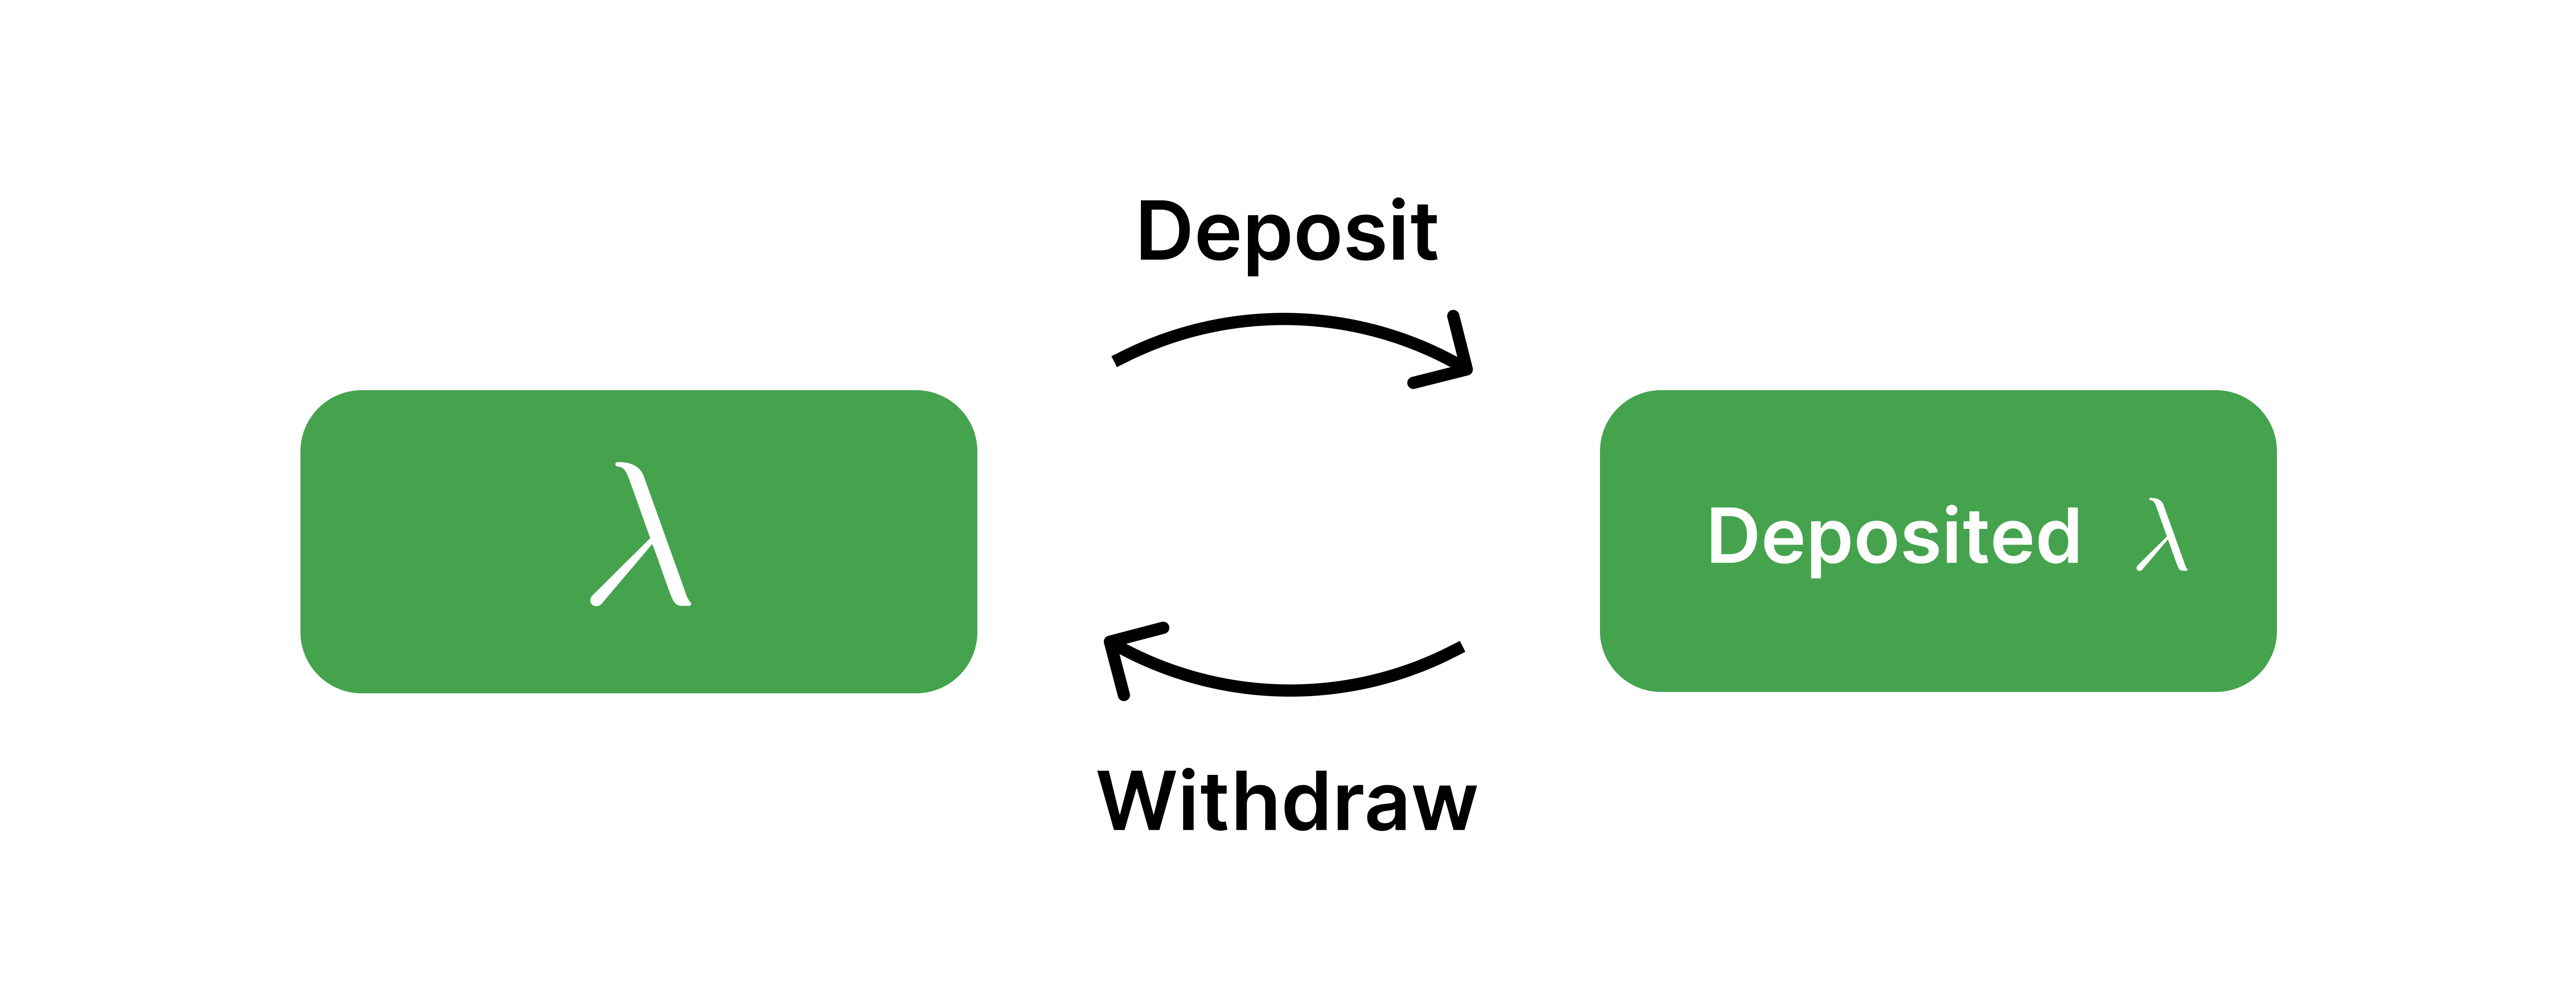
\includegraphics[scale=.16]{Figure1}
    \vspace*{-5mm}
    \caption{Silo}
    \label{fig 1}
\end{figure}

\vspace*{-1mm}
\subsection{Calculating Stalk and Seeds}
\vspace*{-1mm}
A \term{Stalkholder's} total \term{Stalk} is the sum of the \term{Stalk} for each of their \term{Deposits} and \term{Earned} \Bean\ (\hyperlink{ht105}{$\eta^{\bean}$}), such that $\hyperlink{ht105}{\eta^{\bean}} \in \{j \times 10^{-6} \mid j \in \mathbb{N} \}$. 
\term{Earned} \Bean\ are Beans paid to a \term{Stalkholder} after the last time the \term{Stalkholder} called the \code{plant} function (\hyperlink{ht104}{$\eta$}).\footnote{\href{https://bean.money/bip-0}{bean.money/bip-0}}$^{,}$\footnote{\href{https://bean.money/bpp-0}{bean.money/bpp-0}}$^{,}$\footnote{\href{https://bean.money/bip-21}{bean.money/bip-21}} Beans minted to the \term{Silo} are distributed to \term{Stalkholders} and become \term{Earned} \Bean\ 10 blocks past the beginning of the \term{Season} in which they were minted. \term{Earned} \Bean\ automatically earn \term{Stalk}. The next time the \term{Stalkholder} calls the \code{plant} function, \term{Earned} \Bean\ are \term{Deposited} and the associated \term{Seeds} are \term{Planted} to start \term{Growing} \term{Stalk}.

When a \term{Stalkholder} \term{Deposits} \hyperlink{ht126}{$\lambda$}, they update the total number of \hyperlink{ht126}{$\lambda$} \term{Deposited} during \term{Season} $i$ (\hyperlink{ht231}{$Z_i^{\lambda}$}) and its total BDV when \term{Deposited} (\hyperlink{ht123}{$L_i^{\lambda}$}), such that $\hyperlink{ht231}{Z_i^{\lambda}},\ \hyperlink{ht123}{L_i^{\lambda}} \in \{j \times 10^{-6} \mid j \in \mathbb{Z}^{+} \}$, as $\hyperlink{ht231}{Z_i^{\lambda}} \mathrel{+}= z^{\lambda}$ and $\hyperlink{ht123}{L_i^{\lambda}} \mathrel{+}= \hyperlink{ht84}{f^{\lambda}(z^{\lambda})}$. Beanstalk stores a map of each \term{Stalkholder's} \term{Deposits} that are still in the \term{Silo}, from \term{Stalkholder} to \term{Deposit ID} to \term{Deposit} totals (\term{i.e.}, ($\hyperlink{ht231}{Z_i^{\lambda}},\ \hyperlink{ht123}{L_i^{\lambda}}$)). \term{Deposit ID} is the concatenation of the \hyperlink{ht126}{$\lambda$} token address and the maximum \term{Grown} \term{Stalk} per BDV of \hyperlink{ht126}{$\lambda$} at the time of \term{Deposit}.

The \term{Stalk} for a given \term{Deposit} are determined by its duration of \term{Deposit}, BDV when \term{Deposited}, \hyperlink{ht120}{$k^{\lambda}$}, \hyperlink{ht32}{$c^{\lambda}$} and the last \term{Season} the \term{Stalkholder} \term{Mowed} their \term{Grown} \term{Stalk} from \hyperlink{ht126}{$\lambda$} \term{Deposits} (\hyperlink{ht122}{$\varkappa^{\lambda}$}).

The \term{Stalk} during \hyperlink{ht204}{$t$} for a given \term{Deposit} of a \term{Stalkholder} that last \term{Mowed} their \term{Grown} \term{Stalk} from \hyperlink{ht126}{$\lambda$} \term{Deposits} in \hyperlink{ht122}{$\varkappa^{\lambda}$} (\hyperlink{ht121}{$k_{t}^{\lambda}$}), such that $\hyperlink{ht121}{k_{t}^{\lambda}} \in \{j \times 10^{-10} \mid j \in \mathbb{Z}^{+} \}$, is:
$$\hyperlink{ht121}{k_{t}^{\lambda}} = \hyperlink{ht123}{L_i^{\lambda}}\left(\hyperlink{ht120}{k^{\lambda}} + \frac{\hyperlink{ht32}{c^{\lambda}}(\hyperlink{ht122}{\varkappa^{\lambda}} - i)}{10000}\right)$$
A \term{Stalkholder's} total \term{Stalk} during \hyperlink{ht204}{$t$} (\hyperlink{ht118}{$K_t$}), such that $\hyperlink{ht118}{K_t} \in \{j \times 10^{-10} \mid j \in \mathbb{N} \}$, is:
$$\hyperlink{ht118}{K_t} = \sum_{\hyperlink{ht126}{\lambda} \in \hyperlink{ht127}{\Lambda}} \sum_{i=1}^{\hyperlink{ht122}{\varkappa^{\lambda}}} \hyperlink{ht121}{k_{t}^{\lambda}} + \eta^{\bean}$$
The \term{Grown} \term{Stalk} from \term{Seeds} from \hyperlink{ht126}{$\lambda$} \term{Deposits} that can be \term{Mown} during \hyperlink{ht204}{$t$} to start earning Bean seigniorage for a given \term{Deposit} of a \term{Stalkholder} that last \term{Mowed} their \term{Grown} \term{Stalk} from \hyperlink{ht126}{$\lambda$} \term{Deposits} in \hyperlink{ht122}{$\varkappa^{\lambda}$} (\hyperlink{ht101}{$g_{t}^{\lambda}$}), such that $\hyperlink{ht101}{g_{t}^{\lambda}} \in \{j \times 10^{-10} \mid j \in \mathbb{N} \}$, is:
$$\hyperlink{ht101}{g_{t}^{\lambda}} = \hyperlink{ht123}{L_i^{\lambda}}\left(\frac{\hyperlink{ht32}{c^{\lambda}}(t - \hyperlink{ht122}{\varkappa^{\lambda}})}{10000}\right)$$
A \term{Stalkholder's} total \term{Grown} \term{Stalk} that can be \term{Mown} during \hyperlink{ht204}{$t$} (\hyperlink{ht100}{$G_t$}), such that $\hyperlink{ht100}{G_t} \in \{j \times 10^{-10} \mid j \in \mathbb{N} \}$, is:
$$\hyperlink{ht100}{G_t} = \sum_{\hyperlink{ht126}{\lambda} \in \hyperlink{ht127}{\Lambda}} \sum_{i=1}^{\hyperlink{ht122}{\varkappa^{\lambda}}} \hyperlink{ht101}{g_{t}^{\lambda}}$$
The \term{Seeds} for a given \term{Deposit} are determined by its BDV when \term{Deposited} and \hyperlink{ht32}{$c^{\lambda}$}.

The \term{Seeds} during \hyperlink{ht204}{$t$} for a given \term{Deposit} (\hyperlink{ht33}{$c_{t}^{\lambda}$}), such that $\hyperlink{ht33}{c_{t}^{\lambda}} \in \{j \times 10^{-6} \mid j \in \mathbb{Z}^{+} \}$, is:
$$\hyperlink{ht33}{c_{t}^{\lambda}} = \hyperlink{ht32}{c^{\lambda}} \hyperlink{ht123}{L_i^{\lambda}}$$
A \term{Stalkholder's} total \term{Seeds} during \hyperlink{ht204}{$t$} (\hyperlink{ht29}{$C_t$}), such that $\hyperlink{ht29}{C_t} \in \{j \times 10^{-6} \mid j \in \mathbb{N} \}$, is:
$$\hyperlink{ht29}{C_t} = \sum_{\lambda \in \Lambda} \sum_{i=1} \hyperlink{ht33}{c_{t}^{\lambda}}$$
The \term{Plantable} \term{Seeds} associated with a \term{Stalkholder's} \hyperlink{ht105}{$\eta^{\bean}$} that can be \term{Planted} to start earning \term{Grown} \term{Stalk} (\hyperlink{ht106}{$\eta^{c}$}), such that $\hyperlink{ht106}{\eta^{c}} \in \{j \times 10^{-6} \mid j \in \mathbb{N} \}$, is:
$$\hyperlink{ht106}{\eta^{c}} = c^{\bean} \times \hyperlink{ht105}{\eta^{\bean}}$$
When a \term{Stalkholder} \term{Withdraws} \hyperlink{ht126}{$\lambda$}, they must forfeit the number of \term{Stalk}, \term{Seeds}, and \term{Stalk} from \term{Seeds} rewarded to the assets being \term{Withdrawn} and update their map accordingly.

When a \term{Stalkholder} \term{Transfers} \hyperlink{ht126}{$\lambda$}, they must include the number of \term{Stalk}, \term{Seeds}, and \term{Stalk} from \term{Seeds} rewarded to the assets being \term{Transferred} and update their maps accordingly.

When a \term{Stalkholder} \term{Converts} a \term{Deposit}, they update its \term{Grown} \term{Stalk} per BDV to retain its \term{Grown} \term{Stalk} from \term{Seeds}, and BDV if it is higher. When \term{Converting} multiple \hyperlink{ht126}{$\lambda$} \term{Deposits}, their \term{Grown} \term{Stalk} per BDV amounts are averaged together, weighted by their BDVs, and rounded up.

\subsection{Governance}
\vspace*{-1mm}
A robust decentralized governance mechanism must balance the principles of decentralization with resistance to attempted protocol changes, both malicious and ignorant, and the ability to quickly adapt to changing information. In practice, Beanstalk must balance ensuring sufficient time for all ecosystem participants to consider a \term{Beanstalk Improvement Proposal} (\term{BIP}), join the \term{Silo} and cast their votes, with the ability to be quickly upgraded in cases of emergency. 

\subsubsection{Participation}
\vspace*{-1mm}
Any \hyperlink{ht126}{$\lambda$} owner can become a \term{Stalkholder} and participate in Beanstalk governance by \term{Depositing} \hyperlink{ht126}{$\lambda$} into the \term{Silo} to earn \term{Stalk}.

Any \term{Stalkholder} that owns more than \hyperlink{ht119}{$K^{\text{min}}$}, such that $\hyperlink{ht119}{K^{\text{min}}} \in \{j \times 10^{-10} \mid j \in \mathbb{N},\ j \leq 10^{10} \}$, percent of total outstanding \term{Stalk} can submit a \term{BIP} via the \term{Beanstalk Community Multisig}\fref{bean.money/bcm-process} (\term{BCM}). In the future, as the ownership concentration of \term{Stalk} decreases, we expect a \term{BIP} to lower this threshold.

The submitter of a \term{BIP} must own more than $K_{\text{end}}^{\text{min}}$, such that $K_{\text{end}}^{\text{min}} \in \{j \times 10^{-10} \mid j \in \mathbb{N},\ j \leq 10^{10} \}$, percent of total outstanding \term{Stalk} at the end of the \term{Voting Period} in order for a \term{BIP} to be able to pass.

The award for submitting a \term{BIP} that gets accepted (\hyperlink{ht9}{$a^{\text{BIP}}$}), such that $\hyperlink{ht9}{a^{\text{BIP}}} \in \{j \times 10^{-6} \mid j \in \mathbb{N} \}$, is determined by the submitter of the \term{BIP}. If \hyperlink{ht9}{$a^{\text{BIP}}$} is excessively high such that a \term{BIP} that would otherwise be acceptable to the community is voted down because of the award, the open source nature of Beanstalk allows someone else to re-submit an identical \term{BIP} except for a more reasonable \hyperlink{ht9}{$a^{\text{BIP}}$}.

Beanstalk only accepts votes in favor of \term{BIPs}. A \term{Stalkholder's} vote is counted in proportion to their \term{Stalk} at the beginning of the \term{Voting Period} that still exists. \term{Stalkholders} have the ability to delegate their vote to any other user.

\subsubsection{Voting Period}
\vspace*{-1mm}
A \term{Voting Period} opens when the Snapshot\fref{snapshot.org/\#/beanstalkdao.eth} proposal for a \term{BIP} can be voted on and ends approximately 168 \term{Seasons} later, or when it is committed with a supermajority.

\vspace*{2mm}
If at the end of the \term{Voting Period}:
\begin{itemize}[midsep]
    \item Less than or equal to half of the total outstanding \term{Stalk} at the beginning of the \term{Voting Period} that still exists is voting in favor of the \term{BIP}, it fails; and
    \item More than half of the total outstanding \term{Stalk} at the beginning of the \term{Voting Period} that still exists is voting in favor of the \term{BIP}, it passes.
\end{itemize}

If at any time 24 hours or more after the beginning and before the end of the \term{Voting Period} more than two-thirds of the total outstanding \term{Stalk} is voting in favor of the \term{BIP}, it can be committed to the Ethereum blockchain.

\subsubsection{Pause}
In case of a particularly dangerous vulnerability to Beanstalk, the \term{Silo} can \term{Pause} or \term{Unpause} Beanstalk via \term{BIP}. When \term{Paused}, Beanstalk does not accept a \code{gm} function call. When \term{Unpaused}, the \code{gm} function can be called at the beginning of the next hour.

For a given timestamp of last \term{Unpause} (\hyperlink{ht78}{$E_{\Psi}$}) during \term{Season} $t^{'}$, we define $\hyperlink{ht75}{E_{t}^{\text{min}}}\ \forall\ \hyperlink{ht75}{E_{t}^{\text{min}}}$ such that $t^{'} < t$ as:
$$\hyperlink{ht75}{E_{t}^{\text{min}}} = 3600{\left({\left\lfloor\frac{E_{\Psi}}{3600}\right\rfloor} + t - t^{'}\right)}$$

\subsubsection{Beanstalk Improvement Proposals}
Beanstalk implements EIP-2535.\fref{eips.ethereum.org/EIPS/eip-2535} Beanstalk is a diamond with multiple facets. Beanstalk supports multiple simultaneous \term{BIPs} with independent \term{Voting Periods}.

A \term{BIP} has three inputs: (1) a list of facets and functions to add and remove upon commit, (2) a function to run upon commit and (3) the Ethereum address of the contract with (2).

\subsubsection{Beanstalk Community Multisig}
The \term{BCM} address has the exclusive and unilateral ability to \term{Pause} and \term{Unpause} Beanstalk, and submit and commit \term{BIPs}. The \term{BCM} is a 5-of-9 Safe\fref{app.safe.global/eth:0xa9bA2C40b263843C04d344727b954A545c81D043} multisig wallet with anonymous signers consisting of community members and contributors to Beanstalk. The \term{BCM} will provide sufficient notice of the submission, its contents and the submission time before submitting a \term{BIP} to Snapshot. In the future, we expect \term{BIPs} will remove governance entirely, revoking these abilities from the \term{BCM}.

Thus, Beanstalk creates a robust decentralized governance mechanism and consistently improves security, stability and liquidity.

\section{Field}
\vspace*{-1mm}
The Beanstalk peg maintenance mechanism requires the ability to borrow Beans. The \term{Field} is the Beanstalk credit facility. 

Anytime there is \term{Soil} in the \term{Field}, any owner of Beans that are not in the \term{Silo} can \term{Sow} (lend) Beans to Beanstalk in exchange for \term{Pods} and become a \term{Sower}. The \term{Temperature} is the interest rate on Bean loans. The \term{Morning} is the first $Q$, such that ${Q} \in \mathbb{Z}^{+}$, blocks of each \term{Season}. Beanstalk changes the \term{Soil} and \term{Temperature} at the beginning of each block of the \term{Morning} according to the peg maintenance mechanism.

\subsection{Soil}
\vspace*{-1mm}
We define \term{Soil} (\hyperlink{ht170}{$S$}), such that $\hyperlink{ht170}{S} \in \{j \times 10^{-6} \mid j \in \mathbb{N} \}$, as the current number of Beans that can be \term{Sown} in exchange for \term{Pods}. \Bean1 is \term{Sown} in one \term{Soil}. Beanstalk permanently removes \term{Sown} \Bean\ from the Bean supply. 

When Beanstalk is willing to borrow more Beans to remove them from the Bean supply, it creates more \term{Soil}. Beanstalk changes the \term{Minimum Soil} ($S_{t_q}^{\text{min}}$) in block $q$, such that $q \in \mathbb{Z}^{+},\ q \leq Q$, of $t$, such that $S_{t_q}^{\text{min}} \in \{j \times 10^{-6} \mid j \in \mathbb{N} \}$, according to the peg maintenance mechanism. During the \term{Morning} of each \term{Season}, the \term{Minimum Soil} is the result of a Dutch auction.

\subsection{Pods}
\vspace*{-1mm}
\term{Pods} are the primary debt asset of Beanstalk. Beanstalk never defaults on debt: \term{Pods} automatically \term{Yield} from \term{Sown} \Bean\ and never expire.

\newpage

In the future, when the average price of \Bean1 is above its value peg over a \term{Season}, \term{Pods} \term{Ripen} and become \term{Harvestable} (redeemable) for \Bean1 at anytime. \term{Pods} \term{Ripen} on a first in, first out (FIFO) basis: \term{Pods} \term{Yielded} from Beans that are \term{Sown} first \term{Ripen} into \term{Harvestable} \term{Pods} first. \term{Pod} holders can \term{Harvest} their \term{Harvestable} \term{Pods} anytime by calling the \code{harvest} function. There is no penalty for waiting to \term{Harvest} \term{Pods}.

\term{Pods} are transferable. In practice, \term{Pods} are non-callable zero-coupon bonds with priority for maturity represented as a place in line. The number of \term{Pods} that \term{Yield} from \term{Sown} \Bean\ is determined by the \term{Temperature}.

\subsection{Temperature}
\vspace*{-1mm}
We define the \term{Temperature} (\hyperlink{ht110}{$h$}), such that $\hyperlink{ht110}{h} \in \mathbb{Z}^{+}$, as the percentage of additional Beans ultimately \term{Harvested} from 1 \term{Sown} \Bean.

The number of \term{Pods} (\hyperlink{ht40}{$d$}) that \term{Yield} from a given number of \term{Sown} \Bean\ (\hyperlink{ht208}{$u$}), such that $\hyperlink{ht40}{d},\ \hyperlink{ht208}{u} \in \{j \times 10^{-6} \mid j \in \mathbb{Z}^{+} \}$, \term{Sown} with a given \hyperlink{ht110}{$h$} is:
$$\hyperlink{ht40}{d} = \hyperlink{ht208}{u} \times \left(1 + \frac{\hyperlink{ht110}{h}}{100}\right)$$

Beanstalk changes the \term{Maximum Temperature} it is willing to offer each Season ($h_t^{\text{max}}$), such that $h_t^{\text{max}} \in \mathbb{Z}^{+}$, at the beginning of each \term{Season} according to the peg maintenance mechanism. During the \term{Morning} of each \term{Season}, the \term{Temperature} is the result of a Dutch auction.\fref{en.wikipedia.org/wiki/Dutch\_auction} 

\begin{figure}[h!]
    \centering
    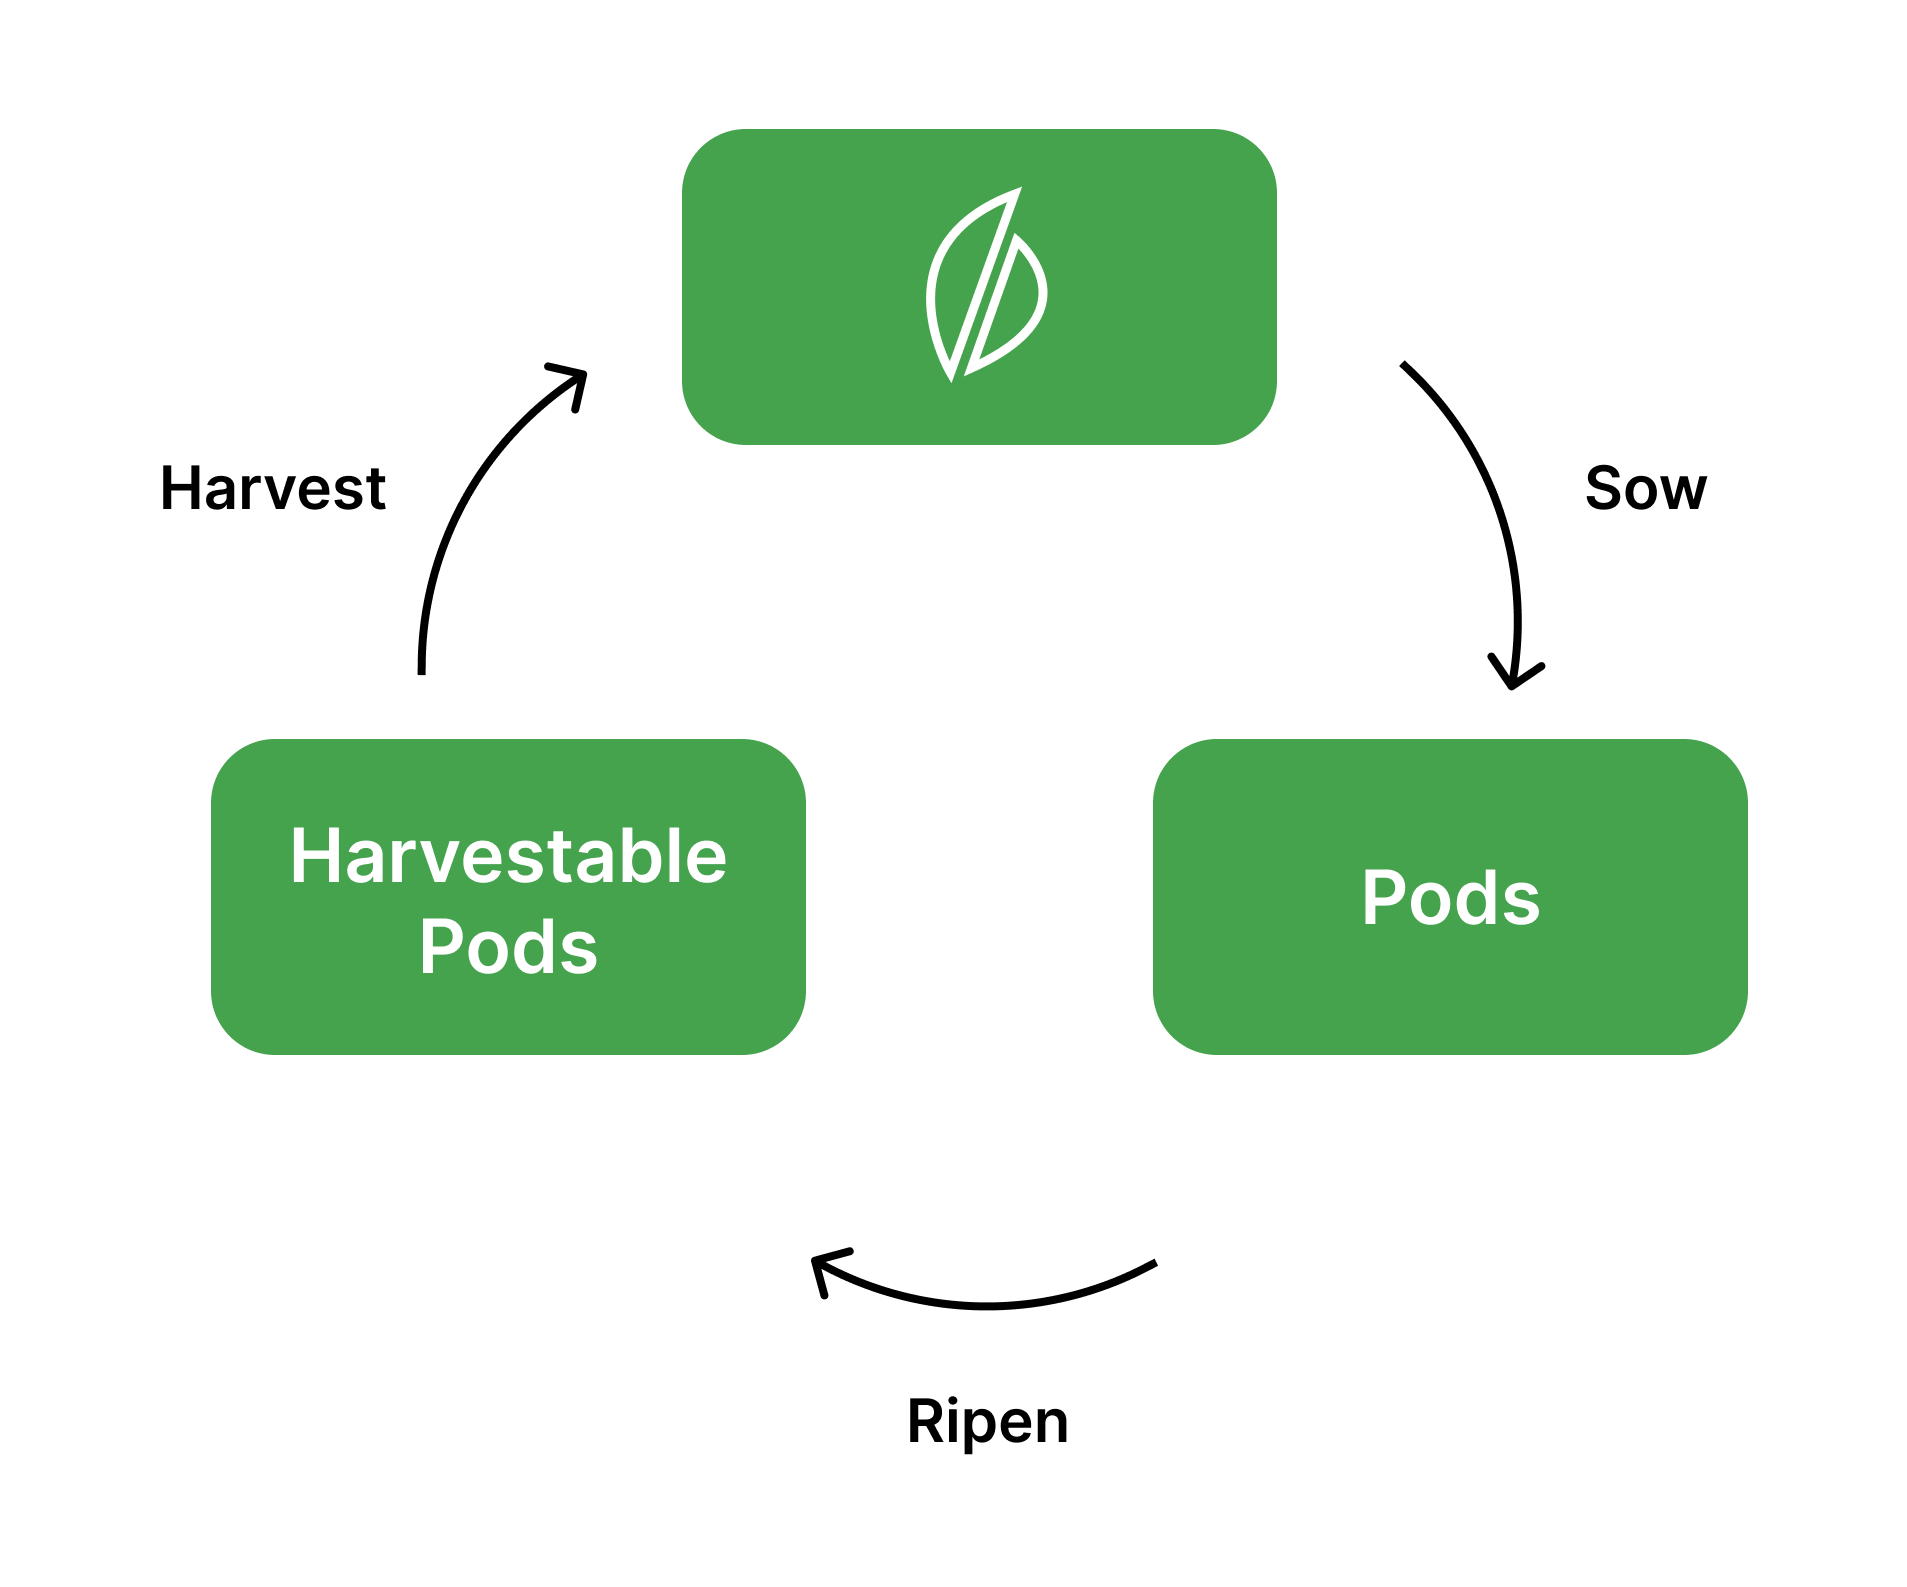
\includegraphics[scale=.14]{Figure2}
    \vspace*{-5mm}
    \caption{Field}
    \label{fig 2}
\end{figure}

\section{Barn}
The \term{Barn} is the Beanstalk recapitalization facility, being used for the Beanstalk \term{Replant}.\footnote{\href{https://bean.money/bfp-72}{bean.money/bfp-72}}$^{,}$\footnote{\href{https://bean.money/barn}{bean.money/barn}}

Anytime there is \term{Available} \term{Fertilizer} (defined below) in the \term{Barn}, any owner of ETH or USDC can buy \term{Fertilizer} from Beanstalk. The \term{Humidity} is the interest rate on \term{Fertilizer} purchases.

\subsection{Fertilizer}
\term{Fertilizer} is a limited debt issuance. \term{Fertilizer} automatically \term{Fertilizes} \term{Sprouts} and never expires.

We define \term{Available} \term{Fertilizer} (\hyperlink{ht217}{$\mathfrak{V}$}) as the number of \term{Fertilizer} that can be bought from Beanstalk in exchange for 1 USDC each, \term{Active} \term{Fertilizer} (\hyperlink{ht12}{$\mathfrak{A}$}) as the number of \term{Fertilizer} that have been bought but have not \term{Fertilized} all associated \term{Sprouts}, and \term{Used} \term{Fertilizer} (\hyperlink{ht209}{$\mathfrak{U}$}), such that $\hyperlink{ht217}{\mathfrak{V}},\ \hyperlink{ht12}{\mathfrak{A}},\ \hyperlink{ht209}{\mathfrak{U}} \in \mathbb{N}$, as the number of \term{Fertilizer} that have been bought and \term{Fertilized} all associated \term{Sprouts}. 

In the future, when the average price of \Bean1 is above its value peg over a \term{Season}, \term{Active} \term{Fertilizer} \term{Fertilizes} \term{Sprouts} such that they become \term{Rinsable} (redeemable) for \Bean1 at anytime. \term{Active} \term{Fertilizer} \term{Fertilizes} a pro-rata portion of \term{Sprouts}, by \term{Fertilizer}. \term{Fertilizer} owners can \term{Rinse} their \term{Rinsable} \term{Sprouts} anytime by calling the \code{rinse} function. There is no penalty for waiting to \term{Rinse} \term{Sprouts}.

\term{Fertilizer} is transferable. In practice, \term{Fertilizer} is a non-callable zero-coupon pari passu bond without a fixed maturity. The number of \term{Sprouts} that \term{Fertilizer} ultimately \term{Fertilizes} is dependent on the \term{Humidity} at its time of purchase.

\subsection{Humidity}
We define the \term{Humidity} (\hyperlink{ht111}{$\mathfrak{H}$}), such that $\hyperlink{ht111}{\mathfrak{H}} \in \{j \times 10^{-1} \mid j \in \mathbb{Z}^{+} \}$, as 1 less than the number of Beans ultimately \term{Fertilized} from 1 \term{Fertilizer} divided by 100. 

The number of \term{Sprouts} (\hyperlink{ht42}{$\mathfrak{d}$}), such that $\hyperlink{ht42}{\mathfrak{d}} \in \{j \times 10^{-6} \mid j \in \mathbb{Z}^{+} \}$, ultimately \term{Fertilized} by \term{Available} \term{Fertilizer} purchased with given \hyperlink{ht111}{$\mathfrak{H}$} (\hyperlink{ht218}{$\mathfrak{V}_\mathfrak{H}$}), such that $\hyperlink{ht218}{\mathfrak{V}_\mathfrak{H}} \in \mathbb{Z}^{+}$, is:
$$\hyperlink{ht42}{\mathfrak{d}} = \hyperlink{ht218}{\mathfrak{V}_\mathfrak{H}} \times \left(1 + \frac{\hyperlink{ht111}{\mathfrak{H}}}{100}\right)$$
The \term{Humidity} is constant each \term{Season}. The \term{Humidity} is 500 prior to the \term{Replant}, after which it is 250 for a full \term{Season} and then decreases by 0.5 each \term{Season} until it reaches 20.

\subsection{Recapitalization}
Beanstalk uses the proceeds from the sale of \term{Fertilizer} to recapitalize value stolen from \term{Stalkholders} in the April 17th, 2022 governance exploit (the \term{Exploit}). Beanstalk will sell enough \term{Fertilizer} to fully recapitalize all non-Beanstalk-native value stolen from \term{Stalkholders}. 

The proportion of a \term{Stalkholder's} \term{Stalk} and \term{Seeds} at the end of the block prior to the \term{Exploit} that have been \term{Revitalized} and can be \term{Enrooted} to begin earning Bean seigniorage and \term{Grown} \term{Stalk}, respectively, is a function of the percentage of \term{Fertilizer} sold.

Non-Beanstalk-native and Beanstalk-native value stolen from \term{Stalkholders} are recapitalized simultaneously via \term{Unripe} assets. \term{Unripe} assets entitle holders to an associated number of \term{Ripe} assets (\term{i.e.}, \Bean\ and BEAN:3CRV Curve LP tokens ($\Phi$), such that $\Phi \in \{j \times 10^{-18} \mid j \in \mathbb{Z}^{+} \}$). The number of \term{Ripe} assets associated with a given \term{Unripe} asset increases as more \term{Fertilizer} is sold. Holders of \term{Unripe} assets can \term{Chop} them and receive a portion of the associated \term{Ripe} asset at anytime. The portion of \term{Ripe} assets that can be received by \term{Chopping} a given \term{Unripe} asset increases as the percentage of \term{Sprouts} \term{Fertilized} increases. Claims to future \term{Ripe} assets are forfeited upon \term{Chopping} the \term{Unripe} asset. 

\subsubsection{Available Fertilizer}
The number of \term{Available} \term{Fertilizer} is the difference between the total \term{Fertilizer} (\hyperlink{ht85}{$\mathfrak{F}$}) and total \term{Fertilizer} sold (\hyperlink{ht174}{$\mathfrak{S}$}), such that $\hyperlink{ht85}{\mathfrak{F}},\ \hyperlink{ht174}{\mathfrak{S}} \in \mathbb{Z}^{+}$. \hyperlink{ht85}{$\mathfrak{F}$} is a function of the current total \term{Unripe} \hyperlink{ht187}{$\Phi$} (\hyperlink{ht230}{$\mathfrak{Z}^{\Phi}$}) and the total \term{Unripe} \hyperlink{ht187}{$\Phi$} at the time of \term{Replant} (\hyperlink{ht232}{$\mathfrak{Z}_{\bigotimes}^{\Phi}$}), such that $\hyperlink{ht235}{\mathfrak{Z}^{\Phi}},\ \hyperlink{ht232}{\mathfrak{Z}_{\bigotimes}^{\Phi}} \in \{j \times 10^{-6} \mid j \in \mathbb{Z}^{+} \}$. \hyperlink{ht174}{$\mathfrak{S}$} is the sum of \term{Active} \term{Fertilizer} and \term{Used} \term{Fertilizer}.

We define \hyperlink{ht85}{$\mathfrak{F}$} for a given \hyperlink{ht230}{$\mathfrak{Z}^{\Phi}$} and \hyperlink{ht232}{$\mathfrak{Z}_{\bigotimes}^{\Phi}$} as:
$$\hyperlink{ht85}{\mathfrak{F}} = \frac{7.7 \times 10^{7} \times \hyperlink{ht230}{\mathfrak{Z}^{\Phi}}}{\hyperlink{ht232}{\mathfrak{Z}_{\bigotimes}^{\Phi}}}$$
We define \hyperlink{ht174}{$\mathfrak{S}$} for a given \hyperlink{ht12}{$\mathfrak{A}$} and \hyperlink{ht209}{$\mathfrak{U}$} as: 
$$\hyperlink{ht174}{\mathfrak{S}} = \hyperlink{ht12}{\mathfrak{A}} + \hyperlink{ht209}{\mathfrak{U}}$$
Therefore, we define \hyperlink{ht217}{$\mathfrak{V}$} for a given \hyperlink{ht85}{$\mathfrak{F}$} and \hyperlink{ht174}{$\mathfrak{S}$} as:
$$\hyperlink{ht217}{\mathfrak{V}} = \hyperlink{ht85}{\mathfrak{F}} - \hyperlink{ht174}{\mathfrak{S}}$$

\subsubsection{Revitalized Stalk and Seeds}
Upon \term{Replant}, \term{Stalkholders} at the end of the block prior to the \term{Exploit} received a portion of their \term{Stalk}, \term{Seeds} and \term{Plantable} \term{Seeds} at the end of the block prior to the \term{Exploit} based on the percentage of \term{Fertilizer} sold prior to \term{Replant} (\hyperlink{ht226}{$\mathfrak{X}_{\bigotimes}$}), such that $\hyperlink{ht226}{\mathfrak{X}_{\bigotimes}} \in \{j \times 10^{-6} \mid j \in \mathbb{Z}^{+} \}$. As the percentage of \term{Fertilizer} sold (\hyperlink{ht225}{$\mathfrak{X}$}), such that $\hyperlink{ht225}{\mathfrak{X}} \in \{j \times 10^{-6} \mid j \in \mathbb{Z}^{+} \}$, increases, additional \term{Stalk} and \term{Seeds} are \term{Revitalized} and can be \term{Enrooted}. \term{Revitalized} \term{Stalk} and \term{Revitalized} \term{Seeds} become \term{Stalk} and \term{Seeds} respectively, upon being \term{Enrooted}. 

We define \hyperlink{ht225}{$\mathfrak{X}$} for a given \hyperlink{ht174}{$\mathfrak{S}$} and \hyperlink{ht85}{$\mathfrak{F}$} as:
$$\hyperlink{ht225}{\mathfrak{X}} = \frac{\hyperlink{ht174}{\mathfrak{S}}}{\hyperlink{ht85}{\mathfrak{F}}}$$
A \term{Stalkholder's} \term{Stalk} upon \term{Replant} (\hyperlink{ht117}{$K_{\bigotimes}$}) given \hyperlink{ht226}{$\mathfrak{X}_{\bigotimes}$} and their \term{Stalk} at the end of the block prior to the \term{Exploit} (\hyperlink{ht116}{$K_{\bigodot}$}), such that $\hyperlink{ht117}{K_{\bigotimes}},\ \hyperlink{ht116}{K_{\bigodot}} \in \{j \times 10^{-10} \mid j \in \mathbb{Z}^{+} \}$, is:
$$\hyperlink{ht117}{K_{\bigotimes}} = \hyperlink{ht226}{\mathfrak{X}_{\bigotimes}} \times \hyperlink{ht116}{K_{\bigodot}}$$
A \term{Stalkholder's} \term{Seeds} upon \term{Replant} (\hyperlink{ht31}{$C_{\bigotimes}$}) given \hyperlink{ht226}{$\mathfrak{X}_{\bigotimes}$}, their \term{Seeds} at the end of the block prior to the \term{Exploit} (\hyperlink{ht30}{$C_{\bigodot}$}) and their \term{Plantable} \term{Seeds} at the end of the block prior to the \term{Exploit} (\hyperlink{ht107}{$\eta_{\bigodot}^c$}), such that $\hyperlink{ht31}{C_{\bigotimes}},\ \hyperlink{ht30}{C_{\bigodot}},\ \hyperlink{ht107}{\eta_{\bigodot}^c} \in \{j \times 10^{-6} \mid j \in \mathbb{Z}^{+} \}$, is:
$$\hyperlink{ht31}{C_{\bigotimes}} = \hyperlink{ht226}{\mathfrak{X}_{\bigotimes}} \times (\hyperlink{ht30}{C_{\bigodot}} + \hyperlink{ht107}{\eta_{\bigodot}^c})$$
The number of \term{Revitalized} \term{Stalk} (\hyperlink{ht203}{${\varphi}_t^K$}), such that $\hyperlink{ht203}{{\varphi}_t^K} \in \{j \times 10^{-10} \mid j \in \mathbb{Z}^{+} \}$, and \term{Revitalized} \term{Seeds} (\hyperlink{ht202}{${\varphi}_t^C$}), such that $\hyperlink{ht202}{{\varphi}_t^C} \in \{j \times 10^{-6} \mid j \in \mathbb{Z}^{+} \}$, that can be \term{Enrooted} by a \term{Stalkholder} during \hyperlink{ht204}{$t$} are functions of the change in \hyperlink{ht225}{$\mathfrak{X}$} (\hyperlink{ht62}{$\Delta \mathfrak{X}$}), such that $\hyperlink{ht62}{\Delta \mathfrak{X}} \in \{j \times 10^{-6} \mid j \in \mathbb{Z}^{+} \}$, between (1) the \term{Season} they last called the \code{enroot} function (\hyperlink{ht201}{$\varphi$}) or (2) the \term{Replant} if they have never \term{Enrooted} their \term{Revitalized} \term{Stalk} and \term{Revitalized} \term{Seeds} (\term{i.e.}, $\hyperlink{ht201}{\varphi} = 0$), and \hyperlink{ht204}{$t$}, and \hyperlink{ht116}{$K_{\bigodot}$} or \hyperlink{ht30}{$C_{\bigodot}$} and \hyperlink{ht107}{$\eta_{\bigodot}^c$}, respectively. 

We define \hyperlink{ht62}{$\Delta \mathfrak{X}$} for a given \term{Stalkholder} that last \term{Enrooted} their \term{Revitalized} \term{Stalk} and \term{Revitalized} \term{Seeds} in \hyperlink{ht201}{$\varphi$} as:
$$\hyperlink{ht62}{\Delta \mathfrak{X}} = \begin{cases} \mathfrak{X}_{t} - \mathfrak{X}_\varphi & \text{if} \; \varphi > 0 \vspace{.3cm} \\ 
\mathfrak{X}_{t} - \hyperlink{ht226}{\mathfrak{X}_{\bigotimes}} & \text{else}\end{cases}$$
We define \hyperlink{ht203}{${\varphi}_t^K$} for a given \hyperlink{ht62}{$\Delta \mathfrak{X}$} and \hyperlink{ht116}{$K_{\bigodot}$} as:
$$\hyperlink{ht203}{{\varphi}_t^K} = \hyperlink{ht62}{\Delta \mathfrak{X}} \times \hyperlink{ht116}{K_{\bigodot}}$$
We define \hyperlink{ht202}{${\varphi}_t^C$} for a given \hyperlink{ht62}{$\Delta \mathfrak{X}$} and \hyperlink{ht30}{$C_{\bigodot}$} as:
$$\hyperlink{ht202}{{\varphi}_t^C} = \hyperlink{ht62}{\Delta \mathfrak{X}} \times (\hyperlink{ht30}{C_{\bigodot}} + \hyperlink{ht107}{\eta_{\bigodot}^c})$$

\subsubsection{Unripe Assets}
Holders of Beans at the end of the block prior to the \term{Exploit} received \term{Unripe} \Bean\ (\hyperlink{ht229}{$\mathfrak{z}^{\bean}$}), such that $\hyperlink{ht233}{\mathfrak{z}^{\bean}} \in \{j \times 10^{-6} \mid j \in \mathbb{Z}^{+} \}$, at a 1:1 ratio.\footnote{\href{https://bean.money/bip-20}{bean.money/bip-20}} Holders of \hyperlink{ht126}{$\lambda$} not \term{Deposited} at the end of the block prior to the \term{Exploit} received \term{Unripe} \hyperlink{ht187}{$\Phi$} (\hyperlink{ht235}{$\mathfrak{z}^{\Phi}$}), such that $\hyperlink{ht235}{\mathfrak{z}^{\Phi}} \in \{j \times 10^{-6} \mid j \in \mathbb{Z}^{+} \}$, at a ratio of 1 \hyperlink{ht235}{$\mathfrak{z}^{\Phi}$} per BDV of \hyperlink{ht126}{$\lambda$} held at the end of the block prior to the \term{Exploit}. Holders of \hyperlink{ht126}{$\lambda$} \term{Deposited} at the end of the block prior to the \term{Exploit} received \hyperlink{ht235}{$\mathfrak{z}^{\Phi}$} at a ratio of 1 $\hyperlink{ht235}{\mathfrak{z}^{\Phi}}$ per the maximum of the BDV of \hyperlink{ht126}{$\lambda$} \term{Deposits} at the end of the block prior to the \term{Exploit} and at the time of \term{Deposit}, per \term{Deposit}. 

\subsubsection{Ripe Assets}
The number of \term{Ripe} assets (\term{i.e.}, \term{Ripe} \Bean\ (\hyperlink{ht158}{$\mathfrak{R}^{\bean}$}), such that $\hyperlink{ht158}{\mathfrak{R}^{\bean}} \in \{j \times 10^{-6} \mid j \in \mathbb{Z}^{+} \}$, and \term{Ripe} \hyperlink{ht187}{$\Phi$} (\hyperlink{ht160}{$\mathfrak{R}^{\Phi}$}), such that $\hyperlink{ht160}{\mathfrak{R}^{\Phi}} \in \{j \times 10^{-18} \mid j \in \mathbb{Z}^{+} \}$), increases as more \term{Fertilizer} is sold.

The change in \term{Ripe} \Bean\ (\hyperlink{ht58}{$\Delta \mathfrak{R}^{\bean}$}) for a given purchase of \term{Fertilizer} (\hyperlink{ht61}{$\Delta \mathfrak{S}_{\Game}$}) is a function of the total \term{Unripe} \Bean\ (\hyperlink{ht229}{$\mathfrak{Z}^{\bean}$}), the \term{Ripe} \Bean\ prior to the purchase (\hyperlink{ht159}{$\mathfrak{R}_{<\Game}^{\bean}$}),  such that $\hyperlink{ht58}{\Delta \mathfrak{R}^{\bean}},\ \hyperlink{ht229}{\mathfrak{Z}^{\bean}},\ \hyperlink{ht159}{\mathfrak{R}_{<\Game}^{\bean}} \in \{j \times 10^{-6} \mid j \in \mathbb{Z}^{+} \}$, \hyperlink{ht85}{$\mathfrak{F}$}, and the \term{Fertilizer} sold prior to the purchase (\hyperlink{ht175}{$\mathfrak{S}_{<\Game}$}),  such that $\hyperlink{ht61}{\Delta \mathfrak{S}_{\Game}},\ \hyperlink{ht175}{\mathfrak{S}_{<\Game}} \in \mathbb{Z}^{+}$.

We define \hyperlink{ht58}{$\Delta \mathfrak{R}^{\bean}$} for a given \hyperlink{ht61}{$\Delta \mathfrak{S}_{\Game}$}, \hyperlink{ht229}{$\mathfrak{Z}^{\bean}$}, \hyperlink{ht159}{$\mathfrak{R}_{<\Game}^{\bean}$}, \hyperlink{ht85}{$\mathfrak{F}$}, \hyperlink{ht175}{$\mathfrak{S}_{<\Game}$} as:
$$\hyperlink{ht58}{\Delta \mathfrak{R}^{\bean}} = \frac{\hyperlink{ht61}{\Delta \mathfrak{S}_{\Game}} \times (\hyperlink{ht229}{\mathfrak{Z}^{\bean}} - \hyperlink{ht159}{\mathfrak{R}_{<\Game}^{\bean}})}{\hyperlink{ht85}{\mathfrak{F}} - \hyperlink{ht175}{\mathfrak{S}_{<\Game}}}$$
The change in \term{Ripe} \hyperlink{ht187}{$\Phi$} (\hyperlink{ht59}{$\Delta \mathfrak{R}^{\Phi}$}), such that $\hyperlink{ht59}{\Delta \mathfrak{R}^{\Phi}} \in \{j \times 10^{-18} \mid j \in \mathbb{Z}^{+} \}$, is the result of calling the \code{calc\_token\_amount} function on the Curve Zap contract\fref{etherscan.io/address/0xA79828DF1850E8a3A3064576f380D90aECDD3359\#code} for a given \hyperlink{ht61}{$\Delta \mathfrak{S}_{\Game}$}.

We define \hyperlink{ht59}{$\Delta \mathfrak{R}^{\Phi}$} for a given \hyperlink{ht61}{$\Delta \mathfrak{S}_{\Game}$} as:
$$\hyperlink{ht59}{\Delta \mathfrak{R}^{\Phi}} = \code{calc\_token\_amount(}\hyperlink{ht187}{\Phi},\ [0.866616 \times \hyperlink{ht61}{\Delta \mathfrak{S}_{\Game}},\ 0,\ \hyperlink{ht61}{\Delta \mathfrak{S}_{\Game}},\ 0],\ true\code{)}$$

\subsubsection{Chopping}
The percentage of \term{Ripe} assets received for \term{Chopping} a pro-rata portion of \term{Unripe} assets (\hyperlink{ht129}{$\mathfrak{M}$}) is a function of the total \term{Sprouts} \term{Fertilized} by \term{Fertilizer} (\hyperlink{ht54}{$\Delta \mathfrak{D}$}) and the total \term{Unfertilized} \term{Sprouts} (\term{i.e.}, \term{Sprouts} not yet \term{Fertilized} by \term{Active} \term{Fertilizer}) (\hyperlink{ht41}{$\mathfrak{D}$}), such that $\hyperlink{ht129}{\mathfrak{M}},\ \hyperlink{ht54}{\Delta \mathfrak{D}},\ \hyperlink{ht41}{\mathfrak{D}} \in \{j \times 10^{-6} \mid j \in \mathbb{Z}^{+} \}$.

We define \hyperlink{ht129}{$\mathfrak{M}$} for a given \hyperlink{ht54}{$\Delta \mathfrak{D}$} and \hyperlink{ht41}{$\mathfrak{D}$} as: 
$$\hyperlink{ht129}{\mathfrak{M}} = \frac{\hyperlink{ht54}{\Delta \mathfrak{D}}}{\hyperlink{ht54}{\Delta \mathfrak{D}} + \hyperlink{ht41}{\mathfrak{D}}} $$

The number of Beans received for \term{Chopping} a given \hyperlink{ht233}{$\mathfrak{z}^{\bean}$} (\hyperlink{ht142}{$\mathfrak{P}^{\bean}$}), such that $\hyperlink{ht142}{\mathfrak{P}^{\bean}} \in \{j \times 10^{-6} \mid j \in \mathbb{Z}^{+} \}$, is a function of \hyperlink{ht129}{$\mathfrak{M}$}, \hyperlink{ht158}{$\mathfrak{R}^{\bean}$} and \hyperlink{ht229}{$\mathfrak{Z}^{\bean}$}.

We define \hyperlink{ht142}{$\mathfrak{P}^{\bean}$} for a given \hyperlink{ht233}{$\mathfrak{z}^{\bean}$}, \hyperlink{ht129}{$\mathfrak{M}$} and \hyperlink{ht158}{$\mathfrak{R}^{\bean}$} as:
$$\hyperlink{ht142}{\mathfrak{P}^{\bean}} = \frac{\hyperlink{ht233}{\mathfrak{z}^{\bean}} \times \hyperlink{ht129}{\mathfrak{M}} \times \hyperlink{ht158}{\mathfrak{R}^{\bean}}}{\hyperlink{ht229}{\mathfrak{Z}^{\bean}}}$$

The number of \hyperlink{ht187}{$\Phi$} received for \term{Chopping} a given \hyperlink{ht235}{$\mathfrak{z}^{\Phi}$} (\hyperlink{ht143}{$\mathfrak{P}^{\Phi}$}), such that $\hyperlink{ht143}{\mathfrak{P}^{\Phi}} \in \{j \times 10^{-18} \mid j \in \mathbb{Z}^{+} \}$, is a function of \hyperlink{ht129}{$\mathfrak{M}$}, \hyperlink{ht174}{$\mathfrak{S}$}, \hyperlink{ht232}{$\mathfrak{Z}_{\bigotimes}^{\Phi}$} and \hyperlink{ht230}{$\mathfrak{Z}^{\Phi}$}.

We define \hyperlink{ht143}{$\mathfrak{P}^{\Phi}$} for a given \hyperlink{ht235}{$\mathfrak{z}^{\Phi}$}, \hyperlink{ht129}{$\mathfrak{M}$}, \hyperlink{ht174}{$\mathfrak{S}$}, \hyperlink{ht232}{$\mathfrak{Z}_{\bigotimes}^{\Phi}$} and \hyperlink{ht230}{$\mathfrak{Z}^{\Phi}$} as:
$$\hyperlink{ht143}{\mathfrak{P}^{\Phi}} = \frac{\hyperlink{ht235}{\mathfrak{z}^{\Phi}} \times \hyperlink{ht129}{\mathfrak{M}} \times \hyperlink{ht174}{\mathfrak{S}} \times \hyperlink{ht232}{\mathfrak{Z}_{\bigotimes}^{\Phi}}}{\hyperlink{ht230}{\mathfrak{Z}^{\Phi}}}$$

\term{Chopped} \term{Unripe} \Bean\ and \hyperlink{ht187}{$\Phi$} are burned (\term{i.e.}, $\hyperlink{ht229}{\mathfrak{Z}^{\bean}} \mathrel{-}= \hyperlink{ht233}{\mathfrak{z}^{\bean}}$, $\hyperlink{ht230}{\mathfrak{Z}^{\Phi}} \mathrel{-}= \hyperlink{ht235}{\mathfrak{z}^{\Phi}}$). \Bean\ and \hyperlink{ht187}{$\Phi$} received for \term{Chopping} are distributed from \term{Ripe} \Bean\ and \hyperlink{ht187}{$\Phi$}, respectively (\term{i.e.}, $\hyperlink{ht158}{\mathfrak{R}^{\bean}} \mathrel{-}= \hyperlink{ht142}{\mathfrak{P}^{\bean}}$, $\hyperlink{ht160}{\mathfrak{R}^{\Phi}} \mathrel{-}= \hyperlink{ht143}{\mathfrak{P}^{\Phi}}$).

\vspace*{5mm}

\begin{figure}[h!]
    \centering
    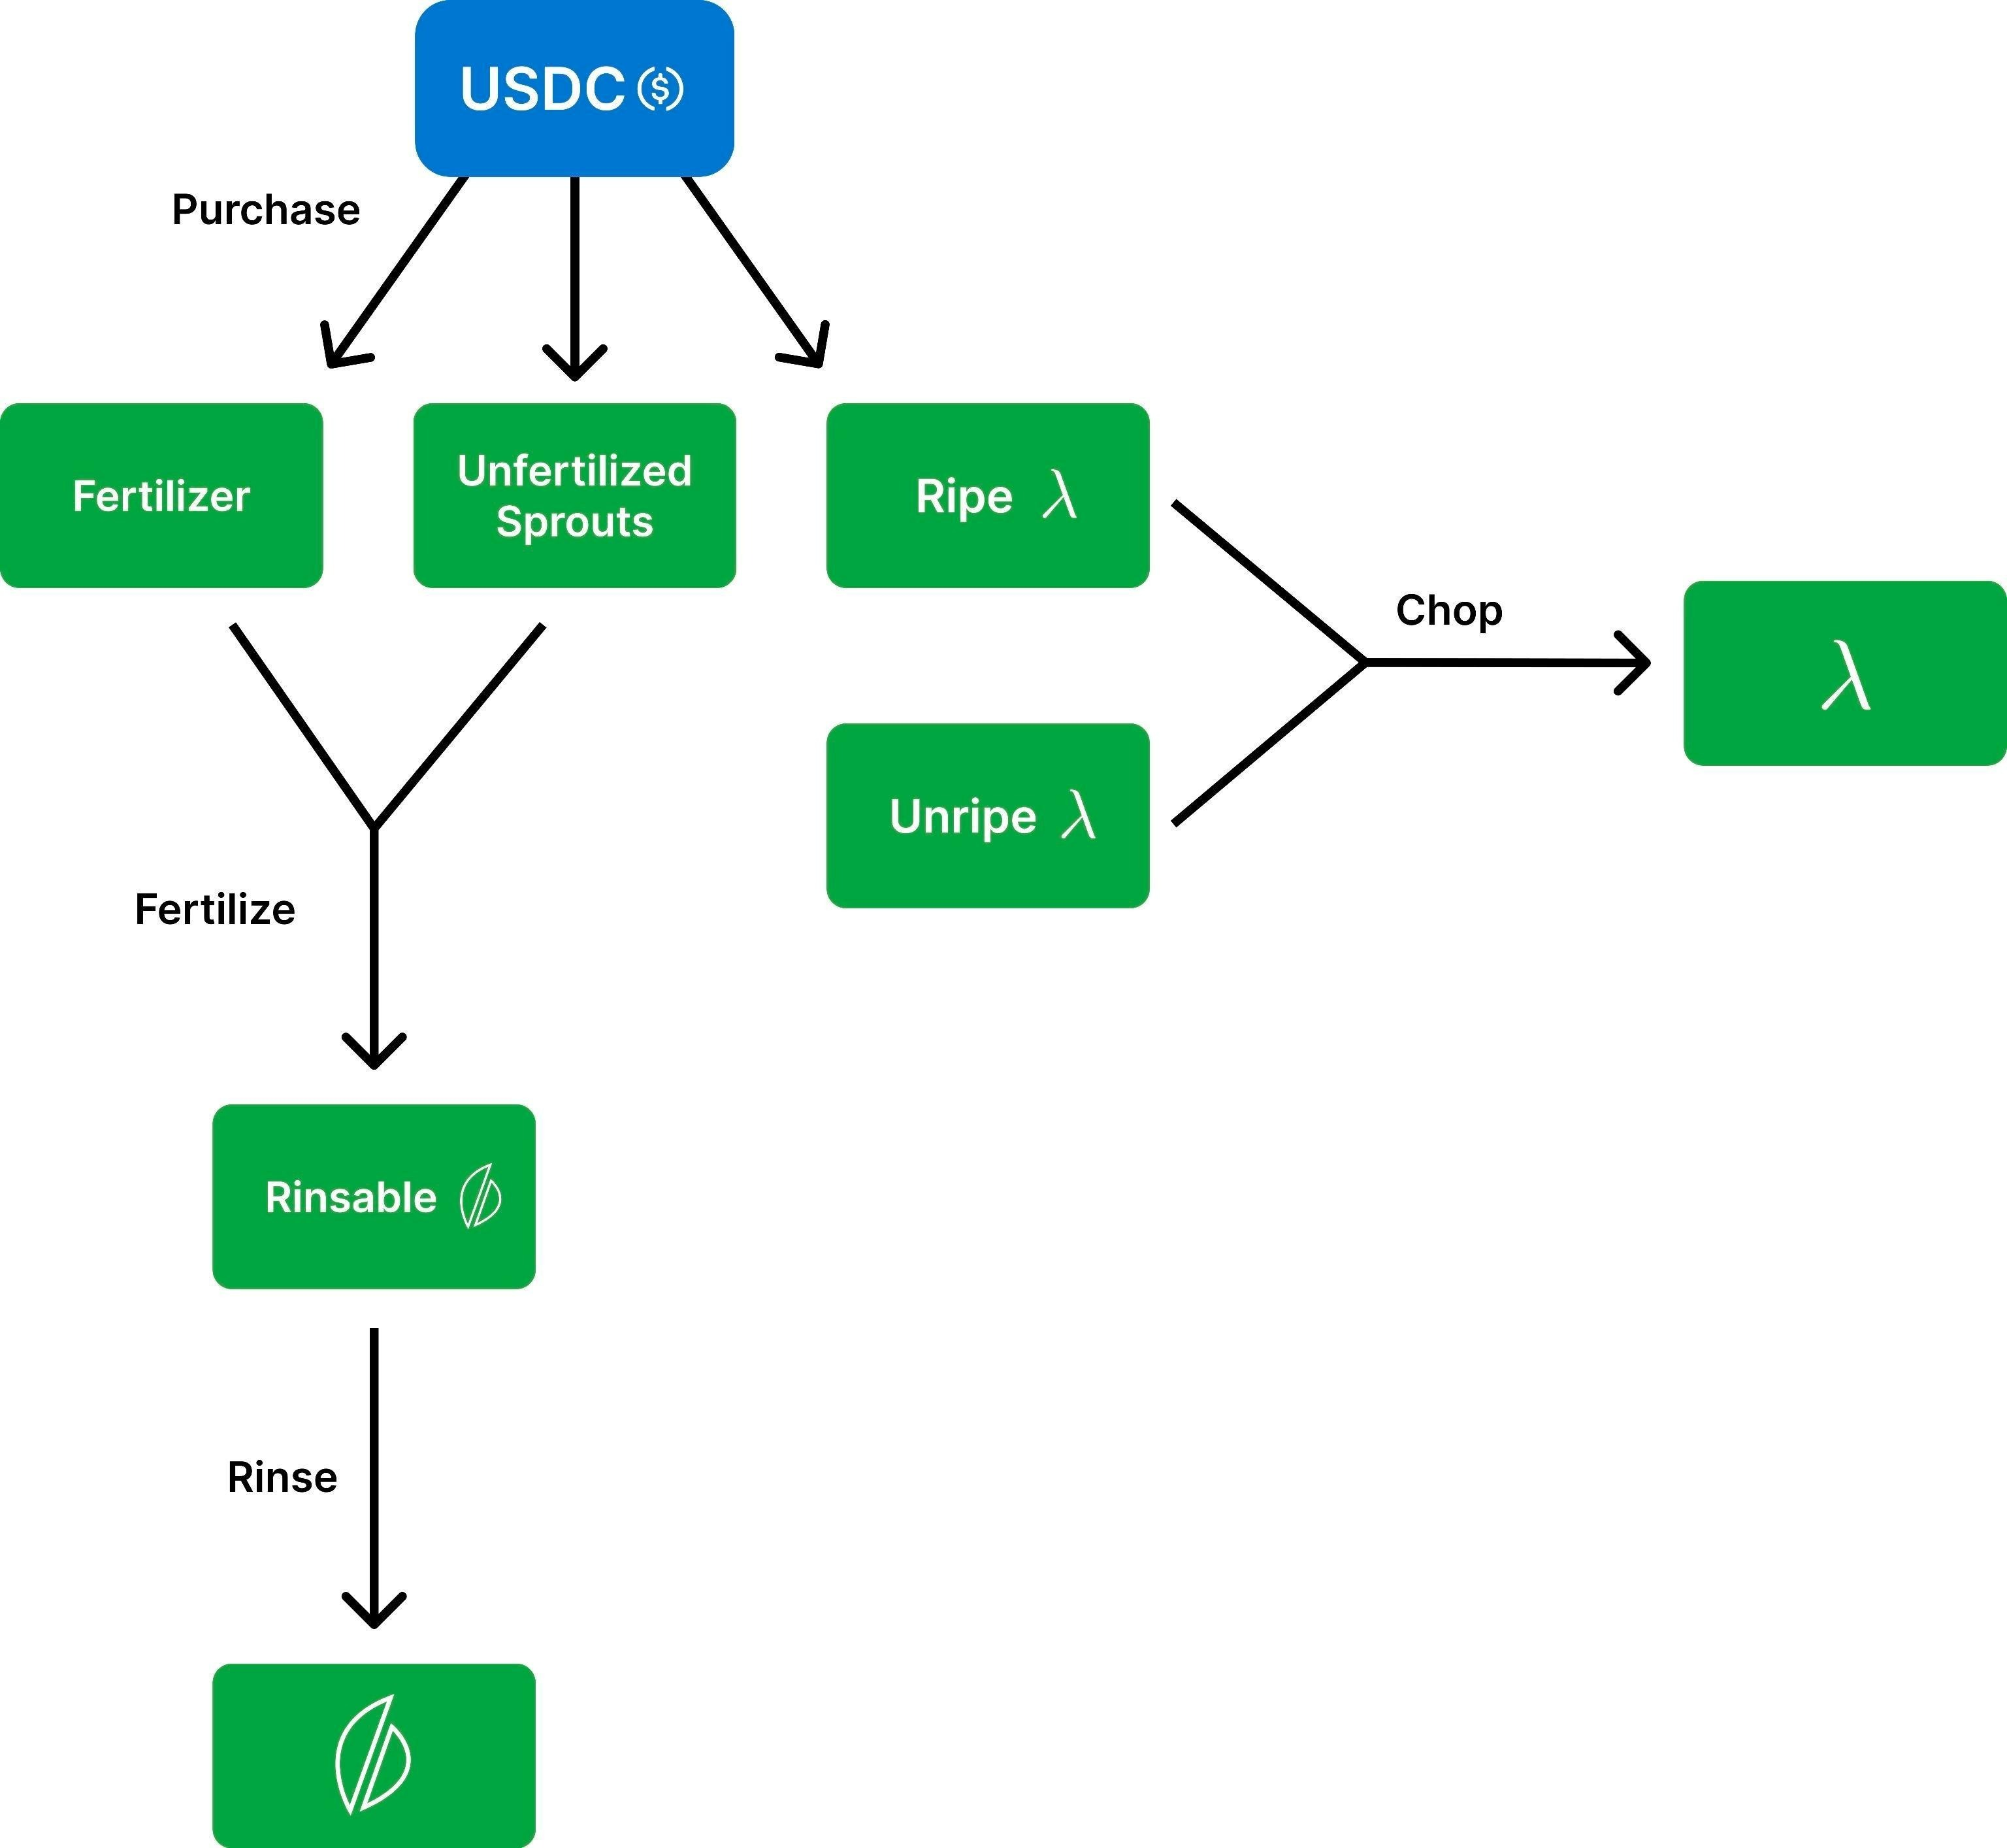
\includegraphics[scale=.14]{Figure3} % mess with scale for desired picture size
    \vspace*{-5mm}
    \caption{Barn}
    \label{fig 3}
\end{figure}

\newpage

\section{Peg Maintenance}

\vspace*{2mm}


Beanstalk faces the fundamental limitation that it cannot fix the price of \Bean1 at its value peg, but instead must encourage widespread participation in peg maintenance through protocol-native financial incentives. Stability is a function of how frequently and regularly the price of \Bean1 crosses, and the magnitudes of price deviations from, its value peg. Beanstalk regularly crosses the price of \Bean1 over its value peg during both long run decreases and increases in demand for Beans.

Beanstalk has four peg maintenance tools available: (1) increase the Bean supply, (2) change the \term{Soil} supply, (3) change the \term{Temperature}, and (4) a \term{Flood} (defined below). At the beginning of every \term{Season}, Beanstalk evaluates its position (\term{i.e.}, price and debt level) and current state (\term{i.e.}, direction and acceleration) with respect to ideal equilibrium, and dynamically adjusts the Bean supply, \term{Soil} supply and \term{Maximum Temperature} to move closer to ideal equilibrium.

\vspace*{2mm}
\subsection{Ideal Equilibrium}
\vspace*{2mm}

Beanstalk is credit based. Beanstalk only fails if it can no longer attract creditors. A reasonable level of debt attracts creditors. Therefore, in addition to the Bean price, the peg maintenance mechanism considers the Beanstalk debt level (defined below). 

Beanstalk is in ideal equilibrium when the Bean price and the Beanstalk debt level are both stable at their optimal levels. In practice, this requires that three conditions are met: (1) the price of \Bean1 is regularly oscillating over its value peg, (2) the Beanstalk debt level is optimal (defined below), and (3) demand for \term{Soil} is steady (defined below). 

Beanstalk affects the supply of and demand for Beans to return to ideal equilibrium in response to the Bean price, the Beanstalk debt level and changing demand for \term{Soil}, by adjusting the Bean supply, \term{Soil} supply and \term{Temperature}. Bean supply increases and \term{Soil} supply changes primarily affect Bean supply. \term{Temperature} changes primarily affect demand for Beans. In order to make the proper adjustments, Beanstalk closely monitors the states of both the Bean and \term{Soil} markets.

In practice, maintaining ideal equilibrium is impossible. Deviations from ideal equilibrium along both axes are normal and expected. As Beanstalk grows, the durations and magnitudes of deviations decrease. 

\vspace*{2mm}
\subsection{Decentralized Price Oracle}
\vspace*{2mm}

One problem native to decentralized stablecoin protocols is the need to be aware of some price without trusting a centralized party to provide it. An oracle delivers external information to smart contracts. A robust decentralized stablecoin requires a tamper-proof, manipulation resistant and decentralized price oracle.

When a price source is not native to the network, decentralized price oracles are complicated to build, expensive to maintain and often inaccurate. Beanstalk leverages network-native decentralized AMMs and non-network-native exogenous value convertible stablecoins to remove these complications, costs and inaccuracies almost entirely, and create an immutable, manipulation resistant and decentralized source for the price of a non-Ethereum-native value peg.

\newpage

Ethereum-native permissionless AMM protocols allow anyone to create new AMMs between at least two ERC-20 Standard tokens. AMMs always offer a price on any size trade, at any time, for a trading fee. AMMs allow continuous trading in either direction by maintaining a liquidity pool of the tokens. The current price is a function of the ratio of the assets in the pool and the AMM pricing formula. Anyone can add liquidity to the pool in exchange for liquidity pool tokens (\hyperlink{LP tokens}{LP tokens}) unique to that liquidity pool. LP token owners often receive a portion of trading fees. Price slippage is proportional to the ratio between the sizes of a trade and the liquidity pool. AMMs with larger liquidity pools serve as more robust price sources.

In general, Beanstalk can issue a Bean with a value peg (\hyperlink{ht216}{$V$}) for \Bean1 equal to any non-network-native asset (\term{e.g.}, \$1) with at least one existing ERC-20 Standard convertible stablecoin (\hyperlink{ht223}{$x$}) (\term{e.g.}, USDC) that (1) offers low-friction convertibility to \hyperlink{ht216}{$V$}, and (2) trades on an AMM against a liquid, decentralized network-native asset with endogenous value (\hyperlink{ht227}{$y$}) (\term{e.g.}, ETH\fref{coinmarketcap.com/academy/article/what-is-wrapped-ethereum-weth}). 

To determine the value of \Bean1 compared to \hyperlink{ht216}{$V$}, Beanstalk can compare (1) an existing liquidity pool (\hyperlink{ht224}{$x$:$y$}) (\term{e.g.}, USDC:ETH) that consists of \hyperlink{ht223}{$x$} and \hyperlink{ht227}{$y$}, and (2) a new liquidity pool (\hyperlink{ht6}{\Bean:$y$}) that consists of Beans and \hyperlink{ht227}{$y$}. The combination of arbitrage opportunities between AMMs and other exchanges, and between \hyperlink{ht223}{$x$} and \hyperlink{ht216}{$V$}, ensures the \hyperlink{ht224}{$x$:$y$} AMM price closely mirrors the exchange rate between \hyperlink{ht216}{$V$} and \hyperlink{ht227}{$y$}. Beanstalk would consider the price of \Bean1 equal to its value peg when the ratios of \hyperlink{ht224}{$x$:$y$} and \hyperlink{ht6}{\Bean:$y$} are equal. 

Decentralized systems are never administered by or dependent on a single individual or centralized organization. Beanstalk can leverage an arbitrary \hyperlink{ht223}{$x$} while minimizing exposure to malicious actions from its operators (\term{e.g.}, censorship) by deriving the price from the ratio between \hyperlink{ht224}{$x$:$y$} and \hyperlink{ht6}{\Bean:$y$}. In instances where there is insufficient inter-block MEV manipulation resistant liquidity for \hyperlink{ht224}{$x$:$y$} on DEX protocols, Beanstalk uses a Chainlink\fref{chain.link} data feed and compares it with the \hyperlink{ht224}{$x$:$y$} AMM prices to facilitate inter-block MEV manipulation resistance.

In practice, Beanstalk never calculates the price of \Bean1. Instead, at the beginning of each \term{Season}, Beanstalk calculates a sum of liquidity and time weighted average shortages and excesses of Beans across \hyperlink{ht6}{\Bean:$y$} liquidity pools on the \term{Oracle} \term{Whitelist} over the previous \term{Season} (\hyperlink{ht50}{$\Delta B_{\overline{t-1}}$}), such that $\hyperlink{ht50}{\Delta B_{\overline{t-1}}} \in \{j \times 10^{-6} \mid j \in \mathbb{N} \}$. Liquidity pools can be added to and removed from the \term{Oracle} \term{Whitelist} via Beanstalk governance.

\hyperlink{ht50}{$\Delta B_{\overline{t-1}}$} can be used to infer the liquidity and time weighted average price of \Bean1 compared to \hyperlink{ht216}{$V$} over the previous \term{Season} (\hyperlink{ht139}{$P_{\overline{t-1}}$}), such that $\hyperlink{ht139}{P_{\overline{t-1}}} \in \{j \times 10^{-6} \mid j \in \mathbb{Z}^{+} \}$. If there was a liquidity and time weighted average shortage of Beans across liquidity pools on the \term{Oracle} \term{Whitelist} over the previous \term{Season} (\term{i.e.}, $0 < \hyperlink{ht50}{\Delta B_{\overline{t-1}}}$), $\hyperlink{ht216}{V} < \hyperlink{ht139}{P_{\overline{t-1}}}$. If there was a liquidity and time weighted average excess of Beans across liquidity pools on the \term{Oracle} \term{Whitelist} over the previous \term{Season} (\term{i.e.}, $\hyperlink{ht50}{\Delta B_{\overline{t-1}}} < 0$), $\hyperlink{ht139}{P_{\overline{t-1}}} < \hyperlink{ht216}{V}$. If there was neither a liquidity and time weighted shortage nor excess of Beans across liquidity pools on the \term{Oracle} \term{Whitelist} over the previous \term{Season} (\term{i.e.}, $\hyperlink{ht50}{\Delta B_{\overline{t-1}}} = 0$), $\hyperlink{ht139}{P_{\overline{t-1}}} = \hyperlink{ht216}{V}$. 

$\hyperlink{ht50}{\Delta B_{\overline{t-1}}} = 0$ for each \term{Season} that contains a \term{Pause} and \term{Unpause}.

Thus, Beanstalk constructs an immutable, manipulation resistant and decentralized price oracle for a non-Ethereum-native value peg.

\subsection{Debt Level}
The \term{Pod Rate} (\hyperlink{ht156}{$R^D$}), such that $\hyperlink{ht156}{R^D} \in \{j \times 10^{-6} \mid j \in \mathbb{N} \}$, represents the Beanstalk debt level relative to the Bean supply.

Beanstalk does not consider \term{Burnt} \Bean, \term{Sown} \Bean, \term{Unfertilized} \term{Sprouts} nor \term{Unharvestable} \term{Pods}, but does consider \term{Rinsable} \term{Sprouts} and \term{Harvestable} \term{Pods}, as part of the total Bean supply.

We define the total Bean supply (\hyperlink{ht16}{$B$}) for a given total Beans minted over all \term{Seasons} (\hyperlink{ht128}{$M$}), such that $\hyperlink{ht16}{B},\ \hyperlink{ht128}{M}, \in \{j \times 10^{-6} \mid j \in \mathbb{Z}^{+} \}$, total \hyperlink{ht9}{$a^{\text{BIP}}$} for all passed \term{BIPs} (\hyperlink{ht7}{$A^{\text{BIP}}$}), total awards for all committed \term{BIPs} (\hyperlink{ht8}{$A^q$}), total Beans minted via \term{BIP} (\hyperlink{ht17}{$B^{\text{BIP}}$}) (\term{e.g.}, \term{Fundraisers}), total \term{Burnt} \Bean\ over all \term{Seasons} (\hyperlink{ht132}{$N^{\bean}$}) and total \term{Sown} \Bean\ over all \term{Seasons} (\hyperlink{ht207}{$U$}), such that $\hyperlink{ht7}{A^{\text{BIP}}},\ \hyperlink{ht8}{A^q},\ \hyperlink{ht17}{B^{\text{BIP}}},\ \hyperlink{ht132}{N^{\bean}},\ U \in \{j \times 10^{-6} \mid j \in \mathbb{N} \}$, as:
$$\hyperlink{ht16}{B} = \hyperlink{ht128}{M} + \hyperlink{ht7}{A^{\text{BIP}}} + \hyperlink{ht8}{A^q} + \hyperlink{ht17}{B^{\text{BIP}}} - (\hyperlink{ht132}{N^{\bean}} + \hyperlink{ht207}{U})$$

We define \hyperlink{ht156}{$R^D$} for a given the total number of \term{Unharvestable} \term{Pods} (\hyperlink{ht38}{$D$}), such that $\hyperlink{ht38}{D} \in \{j \times 10^{-6} \mid j \in \mathbb{N} \}$, and \hyperlink{ht16}{$B$} as:
$$\hyperlink{ht156}{R^D} = \frac{\hyperlink{ht38}{D}}{\hyperlink{ht16}{B}}$$
Beanstalk requires three \hyperlink{ht156}{$R^D$} levels to be set: (1) $R^{D^{\text{lower}}}$, below which debt is considered excessively low, (2) $R^{D^*}$, an optimal level of debt, and (3) $R^{D^{\text{upper}}}$, above or equal to which debt is considered excessively high, such that $R^{D^{\text{lower}}},\ R^{D^*},\ R^{D^{\text{upper}}} \in \{j \times 10^{-6} \mid j \in \mathbb{Z}^{+} \}$. When $R^{D^{\text{lower}}} \leq R^D < R^{D^{\text{upper}}}$ and $\hyperlink{ht156}{R^D} \neq R^{D^*}$ (\term{i.e.}, not optimal), \hyperlink{ht156}{$R^D$} is considered reasonable.

%\vspace*{2.5mm}
\begin{figure}[h!]
    \centering
    \documentclass{standalone}
\usepackage{tikz,pgf}

\begin{document}

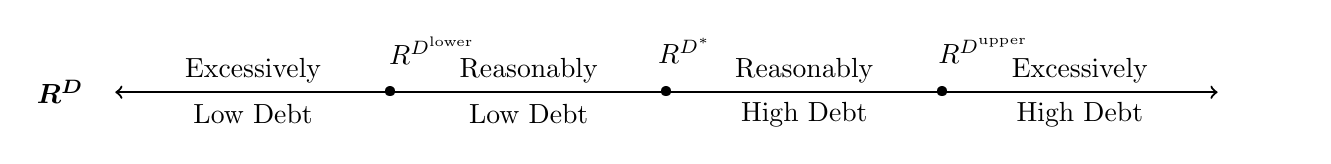
\begin{tikzpicture}[scale=7]

\node [draw=none] at (1.25,0.04) {Excessively};
\node [draw=none] at (1.25,-0.04) {High Debt};

\node [draw=none] at (0.75,0.04) {Reasonably};
\node [draw=none] at (0.75,-0.04) {High Debt};

\node [draw=none] at (0.25,0.04) {Reasonably};
\node [draw=none] at (0.25,-0.04) {Low Debt};

\node [draw=none] at (-0.25,0.04) {Excessively};
\node [draw=none] at (-0.25,-0.04) {Low Debt};

\node [draw=none] at (0.075,0.075) {$R^{D^{\text{lower}}}$};
\node [draw=none] at (0.533,0.075) {$R^{D^*}$};
\node [draw=none] at (1.075,0.075) {$R^{D^{\text{upper}}}$};

\foreach \Point in {0, 0.5, 1}{
    \node[label={[label distance=1mm]:\rotatebox{0}{}}] at (\Point,0) {\textbullet};
}
\draw[thick,<->,color=black] (-0.5,0) -- (1.5,0); % Draw line
\node [draw=none] at (-0.6,0) {\bm{$R^D$}}; % Chart label
\node [draw=none] at (1.6,0)  {\color{white} $R_D$}; % Added to center chart

\end{tikzpicture}

\end{document}
    \vspace*{-7mm}
    \setlength{\belowcaptionskip}{-8pt} % reduce space after caption
    \caption{Debt Level}
    \label{Fig 4}
\end{figure}

\subsection{Position}
The position of Beanstalk with respect to ideal equilibrium can be represented on a graph with axes \hyperlink{ht156}{$R^D$} and $P$, and ideal equilibrium at the origin ($R^{D^*}$, 1). The current state of Beanstalk is determined in part by the position of Beanstalk with respect to ideal equilibrium. 

%\vspace*{2.5mm}
\begin{figure}[h!]
    \centering
    \documentclass{standalone}
\usepackage{tikz,pgf}

\begin{document}

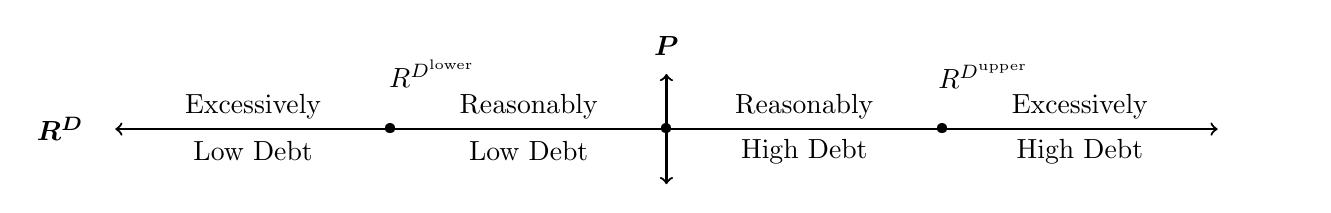
\begin{tikzpicture}[scale=7]

\node [draw=none] at (1.25,0.04) {Excessively};
\node [draw=none] at (1.25,-0.04) {High Debt};

\node [draw=none] at (0.75,0.04) {Reasonably};
\node [draw=none] at (0.75,-0.04) {High Debt};

\node [draw=none] at (0.25,0.04) {Reasonably};
\node [draw=none] at (0.25,-0.04) {Low Debt};

\node [draw=none] at (-0.25,0.04) {Excessively};
\node [draw=none] at (-0.25,-0.04) {Low Debt};

\node [draw=none] at (0.075,0.1) {$R^{D^{\text{lower}}}$};
\node [draw=none] at (1.075,0.095) {$R^{D^{\text{upper}}}$};

\node [draw=none] at (0.5,0.15) {\bm{$P$}};

\foreach \Point in {0, 0.5, 1}{
    \node[label={[label distance=1mm]:\rotatebox{0}{}}] at (\Point,0) {\textbullet};
}
\draw[thick,<->,color=black] (-0.5,0) -- (1.5,0); % Draw horizontal line
\draw[thick,<->,color=black] (0.5,0.1) -- (0.5,-0.1); % Draw vertical line

\node [draw=none] at (-0.6,0) {\bm{$R^D$}}; % Chart label
\node [draw=none] at (1.6,0)  {\color{white} $R_D$}; % Added to center chart

\end{tikzpicture}

\end{document}
    \vspace*{-7mm}
    \caption{Position}
    \label{Fig 5}
\end{figure} 

%\vspace*{-3.5mm} % addedSpace
\subsection{Direction}
%\vspace*{-3.5mm} % addedSpace
The position of Beanstalk with respect to ideal equilibrium changes at the beginning of each \term{Season}. The current state of Beanstalk with respect to ideal equilibrium is determined in part by the direction of this change. 

The direction of change in position of Beanstalk at the beginning of \hyperlink{ht204}{$t$} is considered either toward or away from ideal equilibrium, based on the \term{Pod Rate} at the end of the previous \term{Season} (\hyperlink{ht157}{$R^D_{t-1}$}), such that $\hyperlink{ht157}{R^D_{t-1}} \in \{j \times 10^{-6} \mid j \in \mathbb{Z}^{+} \}$, \hyperlink{ht157}{$R^D_{t-1}$} and \hyperlink{ht139}{$P_{\overline{t-1}}$}. When $\hyperlink{ht216}{V} < \hyperlink{ht139}{P_{\overline{t-1}}}$, debt is paid back; when $\hyperlink{ht139}{P_{\overline{t-1}}} < \hyperlink{ht216}{V}$, debt can only increase or remain constant.

\newpage

Therefore, when $R^{D^*} < \hyperlink{ht157}{R^D_{t-1}}$ (\term{i.e.}, there was more debt than optimal):
\begin{itemize}[topsep=0pt, itemsep=1pt]
    \item If $\hyperlink{ht216}{V} < P_{\overline{t-1}}$, Beanstalk moves toward ideal equilibrium; and
    \item If $P_{\overline{t-1}} \leq \hyperlink{ht216}{V}$, Beanstalk moves away from ideal equilibrium.
\end{itemize}
When $\hyperlink{ht157}{R^D_{t-1}} \leq R^{D^*}$ (\term{i.e.}, there was less debt than optimal):
\begin{itemize}[topsep=0pt, itemsep=1pt]
    \item If $\hyperlink{ht216}{V} \leq P_{\overline{t-1}}$, Beanstalk moves away from ideal equilibrium; or 
    \item If $P_{\overline{t-1}} < \hyperlink{ht216}{V}$, Beanstalk moves toward ideal equilibrium.
\end{itemize}

\begin{figure}[h!]
    \centering
    \advance\leftskip-1cm
    \includetable{figure6}
    \vspace*{2mm}
    \caption{Direction}
    \label{fig 6}
\end{figure}

\subsection{Acceleration}

The current state of Beanstalk with respect to ideal equilibrium also is determined by the rate of change of position of Beanstalk at the beginning of each \term{Season} (\term{i.e.}, its acceleration).

The acceleration of Beanstalk is considered decelerating, steady or accelerating, based on $P_{\overline{t-1}}$ and changing demand for \term{Soil}. Demand for \term{Soil} is considered decreasing, steady or increasing. 

When demand for \term{Soil} is decreasing:
\begin{itemize}[topsep=0pt, itemsep=1pt]
    \item If $\hyperlink{ht216}{V} < P_{\overline{t-1}}$, Beanstalk is decelerating;
    \item If $P_{\overline{t-1}} < \hyperlink{ht216}{V}$, Beanstalk is accelerating;
    \item If $P_{\overline{t-1}} = \hyperlink{ht216}{V}$ and $\hyperlink{ht157}{R^D_{t-1}} \leq R^{D^*}$, Beanstalk is accelerating; and 
    \item If $P_{\overline{t-1}} = \hyperlink{ht216}{V}$ and $R^{D^*} < \hyperlink{ht157}{R^D_{t-1}}$, Beanstalk is decelerating. 
\end{itemize}
When demand for \term{Soil} is steady, Beanstalk is steady.

When demand for \term{Soil} is increasing:
\begin{itemize}[topsep=0pt, itemsep=1pt]
    \item If $\hyperlink{ht216}{V} \leq P_{\overline{t-1}}$, Beanstalk is accelerating; 
    \item If $P_{\overline{t-1}} < \hyperlink{ht216}{V}$, Beanstalk is decelerating;
    \item If $P_{\overline{t-1}} = \hyperlink{ht216}{V}$ and $\hyperlink{ht157}{R^D_{t-1}} \leq R^{D^*}$, Beanstalk is decelerating; and 
    \item If $P_{\overline{t-1}} = \hyperlink{ht216}{V}$ and $R^{D^*} < \hyperlink{ht157}{R^D_{t-1}}$, Beanstalk is accelerating. 
\end{itemize}

\begin{figure}[h!]
    \centering
    \advance\leftskip-1.12cm
    \includetable{figure7}
    \vspace*{2mm}
    \setlength{\belowcaptionskip}{-8pt} % reduce space after caption
    \caption{Acceleration}
    \label{fig 7}
\end{figure}

\vspace*{-3.5mm} % addedSpace
\subsection{Demand for Soil}
\vspace*{-3mm} % addedSpace
In order to properly classify its acceleration, Beanstalk must accurately measure changing demand for \term{Soil}.

The number of \term{Sown} \Bean\ each \term{Season} ($u_t$), such that $u_t \in \{j \times 10^{-6} \mid j \in \mathbb{N} \}$, indicates demand for \term{Soil} over the course of that \term{Season}. The rate of change of $u_t$ from \term{Season} to \term{Season} ($\frac{\partial u_t}{\partial t}$), such that $\frac{\partial u_t}{\partial t} \in \{j \times 10^{-6} \mid j \in \mathbb{N} \}$, indicates changing demand for \term{Soil}.

We define $\frac{\partial u_t}{\partial t}$ over the previous two \term{Seasons}, $u_{t-1}$ and $u_{t-2}$, respectively, as:

$$\frac{\partial u_t}{\partial t} = \frac{u_{t-1}}{u_{t-2}}$$

Beanstalk requires two $\frac{\partial u_t}{\partial t}$ levels to be set: (1) $\frac{\partial u_t}{\partial t}^{\text{lower}}$, below which demand for \term{Soil} is considered decreasing, and (2) $\frac{\partial u_t}{\partial t}^{\text{upper}}$, above or equal to which demand for \term{Soil} is considered increasing, such that $\frac{\partial u_t}{\partial t}^{\text{lower}},\ \frac{\partial u_t}{\partial t}^{\text{upper}} \in \{j \times 10^{-6} \mid j \in \mathbb{Z}^{+} \}$. When $\frac{\partial u_t}{\partial t}^{\text{lower}} \leq \frac{\partial u_t}{\partial t} < \frac{\partial u_t}{\partial t}^{\text{upper}}$, demand for \term{Soil} is considered steady.

\vspace*{-3.5mm} % addedSpace
\begin{figure}[h!]
    \centering
    \documentclass{standalone}
\usepackage{tikz,pgf}

\begin{document}

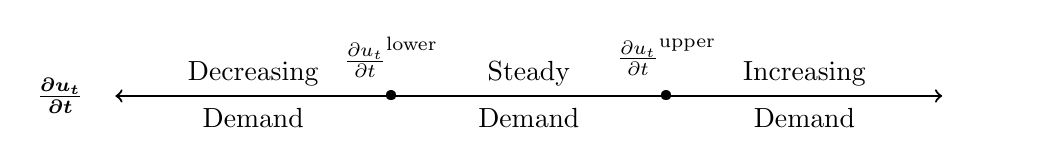
\begin{tikzpicture}[scale=7]

\node [draw=none] at (1,0.04) {Increasing};
\node [draw=none] at (1,-0.04) {Demand};

\node [draw=none] at (0.5,0.04) {Steady};
\node [draw=none] at (0.5,-0.04) {Demand};

\node [draw=none] at (0,0.04) {Decreasing};
\node [draw=none] at (0,-0.04) {Demand};

\node [draw=none] at (0.25,0.07) {$\frac{\partial u_t}{\partial t}^{\text{lower}}$};
\node [draw=none] at (0.75,0.07) {$\frac{\partial u_t}{\partial t}^{\text{upper}}$};

\foreach \Point in {0.25, 0.75}{
    \node[label={[label distance=1mm]:\rotatebox{0}{}}] at (\Point,0) {\textbullet};
}
\draw[thick,<->,color=black] (-0.25,0) -- (1.25,0); % Draw line
\node [draw=none] at (-0.35,0) {\bm{$\frac{\partial u_t}{\partial t}$}}; % Chart label
\node [draw=none] at (1.35,0)  {\color{white} $\frac{\partial u_t}{\partial t}$}; % Added to center chart

\end{tikzpicture}

\end{document}
    % \vspace*{-5mm}
    \vspace*{-10.5mm}
    \caption{Soil Demand Changes From $\frac{\partial u_t}{\partial t}$}
    \label{Fig 8}
\end{figure}

However, when Beans are \term{Sown} in all \term{Soil} in a \term{Season} (defined as $\hyperlink{ht171}{S_t^{\text{end}}} \leq 1$), $\frac{\partial u_t}{\partial t}$ can inaccurately measure changing demand for \term{Soil}. The first time Beans are \term{Sown} in all but at most one \term{Soil} in a \term{Season}, after one or more \term{Seasons} where Beans were not \term{Sown} in all but at most one \term{Soil}, demand for \term{Soil} is considered increasing. When Beans are \term{Sown} in all but at most one \term{Soil} in consecutive \term{Seasons} (\term{i.e.}, $t-1$ and $t-2$), the difference in time it took for the Beans to be \term{Sown} in all but at most one \term{Soil} over the previous two \term{Seasons} (\hyperlink{ht56}{$\Delta E_{t}^{u}$}), such that $\hyperlink{ht56}{\Delta E_{t}^{u}} \in \mathbb{Z}$, can provide a more accurate measurement. 

In order to measure \hyperlink{ht56}{$\Delta E_{t}^{u}$}, Beanstalk logs the time of the first \term{Sow} such that Beans are \term{Sown} in all but at most one \term{Soil} in each \term{Season} (\hyperlink{ht57}{$\Delta E_{t}^{u^{\text{first}}}$}), such that $\hyperlink{ht57}{\Delta E_{t}^{u^{\text{first}}}} \in \mathbb{N}$, as the difference between the Ethereum timestamp of the first \term{Sow} in \hyperlink{ht204}{$t$} such that there is at most one \term{Soil} (\hyperlink{ht76}{$E_{t}^{u^{\text{first}}}$}) and \hyperlink{ht74}{$E_\Xi$}. 

We define \hyperlink{ht57}{$\Delta E_{t}^{u^{\text{first}}}$} for a given \hyperlink{ht76}{$E_{t}^{u^{\text{first}}}$} and \hyperlink{ht74}{$E_\Xi$} as:
$$\hyperlink{ht57}{\Delta E_{t}^{u^{\text{first}}}} = \hyperlink{ht76}{E_{t}^{u^{\text{first}}}} - \hyperlink{ht74}{E_\Xi}$$
If Beans were \term{Sown} in all but at most one \term{Soil} in the first 10 minutes of the previous \term{Season} (\term{i.e.}, $\Delta E_{t-1}^{u^{\text{first}}} < 600$), demand for \term{Soil} is considered increasing. If Beans were \term{Sown} in all but at most one \term{Soil} in both $t-1$ and $t-2$, but $600 \leq \Delta E_{t-1}^{u^{\text{first}}}$, at the beginning of \hyperlink{ht204}{$t$} Beanstalk compares $\Delta E_{t-1}^{u^{\text{first}}}$ with $\Delta E_{t-2}^{u^{\text{first}}}$ to calculate \hyperlink{ht56}{$\Delta E_{t}^{u}$}.

We define \hyperlink{ht56}{$\Delta E_{t}^{u}$} for a given $\Delta E_{t-1}^{u^{\text{first}}}$ and $\Delta E_{t-2}^{u^{\text{first}}}$ as:

$$\hyperlink{ht56}{\Delta E_{t}^{u}} = \Delta E_{t-2}^{u^{\text{first}}} - \Delta E_{t-1}^{u^{\text{first}}}$$

\newpage

If the above condition is met, changing demand for \term{Soil} is measured by \hyperlink{ht56}{$\Delta E_{t}^{u}$}. Beanstalk requires two \hyperlink{ht56}{$\Delta E_{t}^{u}$} levels to be set: (1) $\Delta E_{t}^{u^{\text{lower}}}$, below which demand for \term{Soil} is considered decreasing, and (2) $\Delta E_{t}^{u^{\text{upper}}}$, above which demand for \term{Soil} is considered increasing, such that $\Delta E_{t}^{u^{\text{lower}}},\ \Delta E_{t}^{u^{\text{upper}}} \in \mathbb{Z}$. When $\Delta E_{t}^{u^{\text{lower}}} \leq \hyperlink{ht56}{\Delta E_{t}^{u}} < \Delta E_{t}^{u^{\text{upper}}}$, demand for \term{Soil} is considered steady.

Thus, Beanstalk measures changing demand for \term{Soil}.

% \vspace*{-3mm} % addedSpace
\begin{figure}[h!]
    \centering
    \documentclass{standalone}
\usepackage{tikz,pgf}

\begin{document}

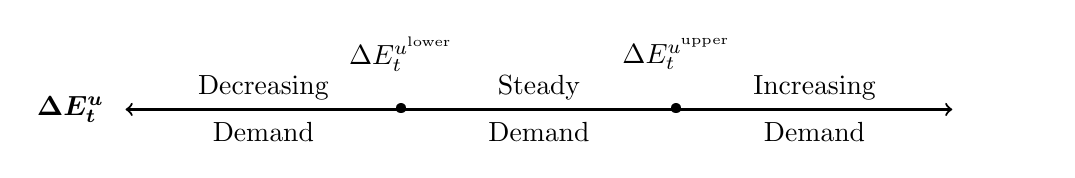
\begin{tikzpicture}[scale=7]

\node [draw=none] at (1,0.04) {Increasing};
\node [draw=none] at (1,-0.04) {Demand};

\node [draw=none] at (0.5,0.04) {Steady};
\node [draw=none] at (0.5,-0.04) {Demand};

\node [draw=none] at (0,0.04) {Decreasing};
\node [draw=none] at (0,-0.04) {Demand};

\node [draw=none] at (0.25,0.1) {$\Delta E_{t}^{u^{\text{lower}}}$};
\node [draw=none] at (0.75,0.1) {$\Delta E_{t}^{u^{\text{upper}}}$};

\foreach \Point in {0.25, 0.75}{
    \node[label={[label distance=1mm]:\rotatebox{0}{}}] at (\Point,0) {\textbullet};
}
\draw[thick,<->,color=black] (-0.25,0) -- (1.25,0); % Draw line
\node [draw=none] at (-0.35,0) {\bm{$\Delta E_{t}^{u}$}}; % Chart label
\node [draw=none] at (1.35,0)  {\color{white} $\Delta E_{t}^{u}$}; % Added to center chart

\end{tikzpicture}

\end{document}
    % \vspace*{-5mm}
    \vspace*{-10.5mm} % reduce space before caption
    \setlength{\belowcaptionskip}{-8pt} % reduce space after caption
    \caption{Soil Demand Changes From $\Delta E_{t}^{u}$}
    \label{Fig 9}
\end{figure}

% \vspace*{-3mm}
% \newpage
\subsection{Current State}
% \vspace*{-4mm}

We define the current state of Beanstalk with respect to ideal equilibrium as the combination of its direction and acceleration with respect to ideal equilibrium. With two potential directions and three potential accelerations, Beanstalk has six potential current states:
% \vspace*{-3.5mm}
\begin{multicols}{2}
\begin{itemize}[midsep]
% \begin{itemize}[topsep=0pt, itemsep=1pt]
    \item Accelerating away from ideal equilibrium;
    \item Steady away from ideal equilibrium;
    \item Decelerating away from ideal equilibrium;
    \item Accelerating toward ideal equilibrium;
    \item Steady toward ideal equilibrium; and
    \item Decelerating toward ideal equilibrium.
\end{itemize}
\end{multicols}

% \vspace*{-5.5mm}
% \vspace*{2.5mm}
\begin{figure}[h!]
    \centering
    \advance\leftskip-1cm
    \includetable{figure10}
    \vspace*{0mm}
    \setlength{\belowcaptionskip}{-8pt} % reduce space after caption
    \caption{Current State}
    \label{fig 10}
\end{figure}

\subsection{Optimal State}

An optimal state of Beanstalk is an optimal current state determined by its current debt level.

We define an optimal state of Beanstalk as accelerating toward ideal equilibrium, or either steady or decelerating toward ideal equilibrium. When $R^D$ is excessively high or low, the optimal state is accelerating toward ideal equilibrium. When $R^D$ is reasonably high or low, the optimal state is either steady or decelerating toward ideal equilibrium.

\begin{figure}[h!]
    \centering
    \advance\leftskip-1cm
    \includetable{figure11}
    \vspace*{2mm}
    \setlength{\belowcaptionskip}{-8pt} % reduce space after caption
    \caption{Optimal State}
    \label{fig 11}
\end{figure}

\subsection{Bean Supply}

At the beginning of each \term{Season}, if $\hyperlink{ht216}{V} < P_{\overline{t-1}}$, Beanstalk increases the Bean supply based on \hyperlink{ht50}{$\Delta B_{\overline{t-1}}$} in addition to the award for successfully calling the \code{gm} function. Up to two thirds of the additional Bean supply increase is used to pay off debt; the remainder is distributed to \term{Stalkholders}.

At the beginning of each \term{Season}, Beanstalk mints $m_t$ Beans, such that $m_t \in \{j \times 10^{-6} \mid j \in \mathbb{Z}^{+} \}$.
We define $m_t$ for a given \hyperlink{ht50}{$\Delta B_{\overline{t-1}}$} and \hyperlink{ht11}{$a_t$} as:
$$m_t = \text{max}(0,\ \hyperlink{ht50}{\Delta B_{\overline{t-1}}}) + \hyperlink{ht11}{a_t}$$
The distribution of the additional mint is dependent on \hyperlink{ht50}{$\Delta B_{\overline{t-1}}$}, \hyperlink{ht41}{$\mathfrak{D}$} and \hyperlink{ht38}{$D$}. If $0 < \frac{\hyperlink{ht50}{\Delta B_{\overline{t-1}}}}{3} \leq \hyperlink{ht41}{\mathfrak{D}}$ (\term{i.e.}, there are at most $\frac{\hyperlink{ht50}{\Delta B_{\overline{t-1}}}}{3}$ \term{Unfertilized} \term{Sprouts}), $\frac{\hyperlink{ht50}{\Delta B_{\overline{t-1}}}}{3}$ \term{Sprouts} are \term{Fertilized} by \term{Active} \term{Fertilizer} and become \term{Rinsable}. If $0 < \hyperlink{ht41}{\mathfrak{D}} < \frac{\hyperlink{ht50}{\Delta B_{\overline{t-1}}}}{3}$ (\term{i.e.}, there are less \term{Unfertilized} \term{Sprouts} than $\frac{\hyperlink{ht50}{\Delta B_{\overline{t-1}}}}{3}$), $\hyperlink{ht41}{\mathfrak{D}}$ \term{Sprouts} are \term{Fertilized} by \term{Active} \term{Fertilizer} and become \term{Rinsable}.

Therefore, the number of \term{Unfertilized} \term{Sprouts} that are \term{Fertilized} by \term{Active} \term{Fertilizer} and become \term{Rinsable} at the beginning of each \term{Season} (\hyperlink{ht55}{$\Delta \mathfrak{D}_t$}), such that $\hyperlink{ht55}{\Delta \mathfrak{D}_t} \in \{j \times 10^{-6} \mid j \in \mathbb{N} \}$, for a given \hyperlink{ht50}{$\Delta B_{\overline{t-1}}$} and \hyperlink{ht41}{$\mathfrak{D}$} is:
$$\hyperlink{ht55}{\Delta \mathfrak{D}_t} = \text{min}\left(\text{max}\left(0,\ \frac{\hyperlink{ht50}{\Delta B_{\overline{t-1}}}}{3}\right),\ \hyperlink{ht41}{\mathfrak{D}}\right)$$

The distribution of the remaining Beans (\term{i.e. $\hyperlink{ht50}{\Delta B_{\overline{t-1}}} - \hyperlink{ht55}{\Delta \mathfrak{D}_t}$}) is dependent on \hyperlink{ht38}{$D$}. If $0 < \hyperlink{ht50}{\Delta B_{\overline{t-1}}} - \hyperlink{ht55}{\Delta \mathfrak{D}_t} < \hyperlink{ht38}{D}$ (\term{i.e.}, there are at most $\hyperlink{ht50}{\Delta B_{\overline{t-1}}} - \hyperlink{ht55}{\Delta \mathfrak{D}_t}$ \term{Unharvestable} \term{Pods}), $\frac{\hyperlink{ht50}{\Delta B_{\overline{t-1}}} - \hyperlink{ht55}{\Delta \mathfrak{D}_t}}{2}$ \term{Pods} \term{Ripen} and become \term{Harvestable} and $\frac{\hyperlink{ht50}{\Delta B_{\overline{t-1}}} - \hyperlink{ht55}{\Delta \mathfrak{D}_t}}{2}$ newly minted Beans are distributed to \term{Stalkholders}. If $0 < \hyperlink{ht38}{D} < \frac{\hyperlink{ht50}{\Delta B_{\overline{t-1}}} - \hyperlink{ht55}{\Delta \mathfrak{D}_t}}{2}$ (\term{i.e.}, there are less \term{Unharvestable} \term{Pods} than $\hyperlink{ht50}{\Delta B_{\overline{t-1}}} - \hyperlink{ht55}{\Delta \mathfrak{D}_t}$), \hyperlink{ht38}{$D$} \term{Pods} \term{Ripen} and become \term{Harvestable} and $\hyperlink{ht50}{\Delta B_{\overline{t-1}}} - (\hyperlink{ht55}{\Delta \mathfrak{D}_t} + \hyperlink{ht38}{D})$ newly minted Beans are distributed to \term{Stalkholders}.

Therefore, the number of \term{Pods} that \term{Ripen} and become \term{Harvestable} at the beginning of each \term{Season} (\hyperlink{ht53}{$\Delta D_t$}), such that $\hyperlink{ht53}{\Delta D_t} \in \{j \times 10^{-6} \mid j \in \mathbb{N} \}$, is:
\vspace*{1mm}
$$\hyperlink{ht53}{\Delta D_t} = \text{min}\left(\text{max}\left(0,\ \frac{\hyperlink{ht50}{\Delta B_{\overline{t-1}}} - \hyperlink{ht55}{\Delta \mathfrak{D}_t}}{2}\right),\ \hyperlink{ht38}{D}\right)$$

\subsection{Soil Supply}

Beanstalk is willing to issue debt every \term{Season}. When $\hyperlink{ht216}{V} \leq \hyperlink{ht139}{P_{\overline{t-1}}}$, the \term{Soil} supply is based on (1) the number of \term{Pods} that \term{Ripen} and become \term{Harvestable} at the beginning of the \term{Season}, (2) the \term{Temperature} in block $q$ of $t$ ($h_{t_q}$), such that $h_{t_q} \in \mathbb{Z}^{+}$, and (3) \hyperlink{ht157}{$R^D_{t-1}$}. When $\hyperlink{ht139}{P_{\overline{t-1}}} < \hyperlink{ht216}{V}$, the \term{Soil} supply is also based on \hyperlink{ht50}{$\Delta B_{\overline{t-1}}$}.

We define the $S_{t_q}^{\text{min}}$ Beanstalk has outstanding for a given \hyperlink{ht53}{$\Delta D_t$}, {$h_{t_q}$} and \hyperlink{ht157}{$R^D_{t-1}$} as:

\vspace*{2mm}

$$S_{t_q}^{\text{min}} = \begin{cases} \dfrac{0.5 \times \hyperlink{ht53}{\Delta D_t}}{1 + \frac{h_{t_q}}{100}} & \text{if} \; R^{D^{\text{upper}}} \leq \hyperlink{ht157}{R^D_{t-1}} \vspace{.3cm} \\ 
\dfrac{\hyperlink{ht53}{\Delta D_t}}{1 + \frac{h_{t_q}}{100}} & \text{if} \; R^{D^{\text{lower}}} < \hyperlink{ht157}{R^D_{t-1}} \vspace{.3cm} \\ 
\dfrac{1.5 \times \hyperlink{ht53}{\Delta D_t}}{1 + \frac{h_{t_q}}{100}} & \text{else} \end{cases}$$

\vspace*{2mm}

Beanstalk calculates the \term{Maximum Soil} ($S_{t_q}^{\text{max}}$), such that $S_{t_q}^{\text{max}} \in \{j \times 10^{-6} \mid j \in \mathbb{N} \}$, in block $q$ of $t$ for a given \hyperlink{ht50}{$\Delta B_{\overline{t-1}}$} and $S_{t_q}^{\text{min}}$ as:

$$S_{t_q}^{\text{max}} = \text{max}(-\hyperlink{ht50}{\Delta B_{\overline{t-1}}},\ S_{t_q}^{\text{min}})$$

\subsection{Temperature}
%\vspace*{1mm}
Beanstalk regularly crosses the price of \Bean1 over its value peg during long run decreases and increases in demand for Beans primarily by adjusting the \term{Maximum Temperature} in an attempt to maintain an optimal state, or to move from its current state into an optimal state. The \term{Temperature} increases each block of the \term{Morning} of each \term{Season} according to a Dutch auction. 

\subsubsection{Maximum Temperature}
The \term{Maximum Temperature} change at the beginning of $t$ is determined by $R^D_{t-1}$ and the current state of Beanstalk with respect to ideal equilibrium. When $R^D_{t-1}$ is excessively high or low, Beanstalk changes the \term{Maximum Temperature} more aggressively.

When $R^{D^{\text{upper}}} \leq \hyperlink{ht157}{R^D_{t-1}}$ (\term{i.e.}, the debt level was excessively high):
\begin{itemize}[midsep]
    \item If the current state is accelerating or steady away from ideal equilibrium, the \term{Maximum Temperature} is raised 3\%;
    \item If the current state is decelerating away from ideal equilibrium, the \term{Maximum Temperature} is raised 1\%;
    \item If the current state is decelerating toward ideal equilibrium, the \term{Maximum Temperature} is kept constant;
    \item If the current state is steady toward ideal equilibrium, the \term{Maximum Temperature} is lowered 1\%; and
    \item If the current state is accelerating toward ideal equilibrium, the \term{Maximum Temperature} is lowered 3\%.
\end{itemize}

\newpage

When $R^{D^*} \leq \hyperlink{ht157}{R^D_{t-1}} < R^{D^{\text{upper}}}$ (\term{i.e.}, the debt level was reasonably high):
\begin{itemize}[midsep]
    \item If the current state is accelerating or steady away from ideal equilibrium, the \term{Maximum Temperature} is raised 3\%;
    \item If the current state is decelerating away from ideal equilibrium, the \term{Maximum Temperature} is raised 1\%;
    \item If the current state is decelerating toward ideal equilibrium, the \term{Maximum Temperature} is kept constant;
    \item If the current state is steady toward ideal equilibrium, the \term{Maximum Temperature} is lowered 1\%; and
    \item If the current state is accelerating toward ideal equilibrium, the \term{Maximum Temperature} is lowered 3\%.
\end{itemize}

When $ R^{D^{\text{lower}}} \leq \hyperlink{ht157}{R^D_{t-1}} < R^{D^*}$ (\term{i.e.}, the debt level was reasonably low):
\begin{itemize}[midsep]
    \item If the current state is accelerating or steady away from ideal equilibrium, the \term{Maximum Temperature} is lowered 3\%;
    \item If the current state is decelerating away from ideal equilibrium, the \term{Maximum Temperature} is lowered 1\%;
    \item If the current state is decelerating toward ideal equilibrium, the \term{Maximum Temperature} is kept constant;
    \item If the current state is steady toward ideal equilibrium, the \term{Maximum Temperature} is raised 1\%; and
    \item If the current state is accelerating toward ideal equilibrium, the \term{Maximum Temperature} is raised 3\%.
\end{itemize}

When $\hyperlink{ht157}{R^D_{t-1}} < R^{D^{\text{lower}}}$ (\term{i.e.}, the debt level was excessively low):
\begin{itemize}[midsep]
    \item If the current state is accelerating or steady away from ideal equilibrium, the \term{Maximum Temperature} is lowered 3\%;
    \item If the current state is decelerating away from ideal equilibrium, the \term{Maximum Temperature} is lowered 1\%;
    \item If the current state is decelerating toward ideal equilibrium, the \term{Maximum Temperature} is kept constant;
    \item If the current state is steady toward ideal equilibrium, the \term{Maximum Temperature} is raised 1\%; and
    \item If the current state is accelerating toward ideal equilibrium, the \term{Maximum Temperature} is raised 3\%.
\end{itemize}

\begin{figure}[h!]
    \centering
    \advance\leftskip-1cm
    \includetable{figure12}
    \vspace*{2mm}
    \caption{Maximum Temperature Changes From Current State and $R^D_{t-1}$}
    \label{fig 12}
\end{figure}

\begin{figure}[h!]
    \centering
    \advance\leftskip-1cm
    \includetable{figure13}
    \vspace*{2mm}
    \caption{Maximum Temperature Changes From $P_{\overline{t-1}}$, Demand for Soil Changes and $R^D_{t-1}$}
    \label{fig 13}
\end{figure}

\subsubsection{Morning}
The \term{Temperature} increases logarithmically in each block of the \term{Morning} of $t$ based on $h_t^{\text{max}}$, $Q$, and a control variable ($\sigma$), such that $\sigma \in \mathbb{Z}^{+}$, as:

$$ h_{t_q} =
\begin{cases}
{1} & \text{if} \; q = 0 \\
{\text{max}(h_t^{\text{max}}*log_{Q\sigma+1}(q\sigma+1),\ 1)} & \text{if} \; 0 < q < Q \\
{h_t^{\text{max}}} & \text{else}
\end{cases} 
$$

Thus, Beanstalk changes the \term{Temperature} to regularly cross the price of \Bean1 over its value peg during long run decreases and increases in demand for Beans.

\subsection{Flood}

Beanstalk sells newly minted Beans on the open market during long run increases in demand for Beans when increasing the Bean supply and lowering the \term{Maximum Temperature} has not crossed the average nor current prices of \Bean1 over its value peg at the end of a \term{Season}.

If $\hyperlink{ht216}{V} < \hyperlink{ht139}{P_{\overline{t-1}}}$, it is \term{Raining}. If it is \term{Raining} and $\hyperlink{ht157}{R^D_{t-1}} < R^{D^{\text{lower}}}$, it \term{Floods} at the beginning of the next \term{Season}. At the beginning of each \term{Season} during a \term{Flood}, Beanstalk returns the price of \Bean1 in each liquidity pool on the \term{Flood} \term{Whitelist} to its value peg by minting additional Beans and selling them directly in the pools. Liquidity pools can be added to and removed from the \term{Flood Whitelist} via Beanstalk governance. Proceeds from the sale are distributed to \term{Stalkholders} at the beginning of \hyperlink{ht204}{$t$} in proportion to their \term{Stalk} holdings when it began to \term{Flood}. At the beginning of the first \term{Season} after the \term{Flood} began, all \term{Pods} that grew from Beans \term{Sown} before the \term{Flood} \term{Ripen} and become \term{Harvestable}.

\newpage

The number of Beans that are minted and sold to return the price of \Bean1 to its value peg (\hyperlink{ht49}{$\Delta B_{t-1}$}), such that $\hyperlink{ht49}{\Delta B_{t-1}} \in \{j \times 10^{-6} \mid j \in \mathbb{N} \}$, is calculated from the sum of differences between the optimal number of Beans and the number of Beans in each \hyperlink{ht6}{\Bean:$y$} liquidity pool on the \term{Flood} \term{Whitelist} at the end of the previous \term{Season}.

In a \term{Flood}, $m_t$ for a given number of \term{Unharvestable} \term{Pods} that grew prior to the \term{Flood} (\hyperlink{ht39}{$D_{\gamma}$}), such that $\hyperlink{ht39}{D_{\gamma}} \in \{j \times 10^{-6} \mid j \in \mathbb{N} \}$, \hyperlink{ht11}{$a_t$}, $\hyperlink{ht50}{\Delta B_{\overline{t-1}}}$, and \hyperlink{ht49}{$\Delta B_{t-1}$} is:
$$m_t = \hyperlink{ht39}{D_{\gamma}} + \hyperlink{ht11}{a_t} + \hyperlink{ht50}{\Delta B_{\overline{t-1}}} + \hyperlink{ht49}{\Delta B_{t-1}}$$
Thus, Beanstalk regularly crosses the price of \Bean1 over its value peg during both long run increases and decreases in demand for Beans.

\vspace*{-1.3mm}
\section{Market}
\vspace*{-1.3mm}

Current DEXs are unable to attract liquidity without offering protocol-native emissions derived primarily from AMM trading fees. Beanstalk's ability to attract liquidity without fee-based emissions allows it to create a DEX without trading fees. The \term{Market} is the Beanstalk-native DEX. Specifications of the \term{Market} are outside the scope of this whitepaper. For information on the \term{Market}, refer to the \hyperlink{section.14}{Appendix}.

\vspace*{-1.3mm}
\section{Depot}
\vspace*{-1.3mm}

Current complex interactions with Ethereum-native protocols are tedious, cumbersome and expensive. The \term{Depot} facilitates complex, gas-efficient interactions with other Ethereum-native protocols in a single transaction. Any protocol with a \term{Pipeline} to the \term{Depot} can be used via Beanstalk in a single transaction. \term{Pipelines} to the \term{Depot} can be added via Beanstalk governance. The specifications of specific \term{Pipelines} are outside the scope of this whitepaper. For information on the \term{Depot}, refer to the \hyperlink{section.14}{Appendix}.

\vspace*{-1.3mm}
\section{Economics}
\vspace*{-1.3mm}

Beanstalk is designed from economic first principles to increase trustlessness, stability and liquidity over time.

\vspace*{-1.3mm}
\subsection{Ownership Concentration}
\vspace*{-1.3mm}

A design that lowers the Gini coefficient\fref{wikipedia.org/wiki/Gini\_coefficient} of Beans and \term{Stalk} over time is essential to censorship resistance.

Older \term{Deposits} have their \term{Stalk} from \term{Seeds} diluted relative to newer \term{Deposits} every \term{Season}. Therefore, newly minted Beans are more widely distributed over time.

Beanstalk does not require a pre-mine. The first 100 Beans are created when the \code{init} function is called to deploy Beanstalk.

\vspace*{-1.3mm}
\subsection{Strong Credit}
\vspace*{-1.3mm}

Beanstalk is credit based and only fails if it can no longer attract creditors. A reasonable level of debt, strong credit history and competitive interest rate attract creditors. 

Beanstalk changes the \term{Temperature} to return \hyperlink{ht156}{$R^D$} to $R^{D^*}$ while regularly crossing the price of \Bean1 over its value peg. Beanstalk acts more aggressively when \hyperlink{ht156}{$R^D$} is excessively high or low.

Beanstalk never defaults on debt and is willing to issue \term{Pods} every \term{Season}. 

\vspace*{-1.3mm}
\subsection{Marginal Rate of Substitution}
\vspace*{-1.3mm}

There are a wide variety of opportunities Beanstalk has to compete with for creditors. Therefore, Beanstalk does not define an optimal \term{Temperature}, but instead adjusts it to move closer to ideal equilibrium. 

\vspace*{-1.3mm}
\subsection{Low Friction}
\vspace*{-1.3mm}

Minimizing the cost of using Beans and barriers to the \term{Farm} maximize utility for users and appeal to creditors. The \term{Depot} realizes the full benefits of composability on Ethereum.

The FIFO \term{Pod} \term{Harvest} schedule allows smaller \term{Sowers} to participate in peg maintenance and decreases the benefit of large scale price manipulation. The combination of non-expiry, the FIFO \term{Harvest} schedule, transferability and a liquid secondary market (see \hyperlink{subsection.14.5}{Appendix}) enables \term{Sowers} to \term{Sow} Beans as efficiently as possible. By maximizing the efficiency of the \term{Soil} market, Beanstalk minimizes its cost to attract creditors, the durations and magnitudes of price deviations below its value peg, and excess \term{Pod} issuance.

\vspace*{-1.3mm}
\subsection{Equilibrium}
\vspace*{-1.3mm}

Equilibrium is a state of equivalent marginal quantity supplied and demanded. Beanstalk affects the supply of and demand for Beans to regularly cross the equilibrium price of \Bean1 over its value peg. 

While Beanstalk can arbitrarily increase the Bean supply when the equilibrium price of \Bean1 is above its value peg, Beanstalk cannot arbitrarily decrease the Bean supply when the equilibrium price of \Bean1 is below it. Beanstalk relies on the codependence between the equilibria of Beans and \term{Soil} to work around this limitation. 

In order to \term{Sow} Beans, they must be acquired (\term{i.e.}, marginal demand for \term{Soil} affects marginal demand for Beans). The marginal demand for \term{Soil} and Beans are functions of the \term{Temperature} and the Bean price. By changing the \term{Temperature}, Beanstalk affects decreases in the Bean supply and changes in demand for Beans. 

\vspace*{-1.3mm}
\subsection{Incentives}
\vspace*{-1.3mm}

Beanstalk-native financial incentives consistently increase trustlessness, stability and liquidity over time by coordinating independently financially motivated actors (\term{i.e}, \term{Stalkholders} and \term{Sowers}). 

The \term{Stalk System} incentivizes (1) leaving assets \term{Deposited} in the \term{Silo} continuously by creating opportunity cost to \term{Withdraw} assets from the \term{Silo}, (2) adding value to liquidity pools with Beans by rewarding more \term{Seeds} to \term{Deposited} LP tokens than \term{Deposited} \Bean, and (3) returning the price of \Bean1 to its value peg by allowing \term{Conversions} within the \term{Silo} without forfeiting \term{Stalk}.

Beanstalk is governed by \term{Stalkholders}. Anyone with \term{Stalk} stands to profit from future growth of Beanstalk, but are not owed anything by Beanstalk. 

When $P_{\overline{t}} < \hyperlink{ht216}{V}$, there is an incentive to \term{Withdraw} assets from the \term{Silo}. The \term{Stalk System} reduces this incentive significantly.

When $\hyperlink{ht216}{V} < P_{\overline{t}}$, there is an incentive to buy Beans to earn a portion of the upcoming Bean seigniorage. This is exacerbated when \hyperlink{ht156}{$R^D$} is lower. The combination of the commitment to automatically return the price of \Bean1 to its value peg and distribute proceeds from the sale to current \term{Stalkholders} based on \term{Stalk} ownership when the \term{Flood} began removes this incentive entirely during \term{Seasons} where \hyperlink{ht157}{$R^D_{t-1}$} is excessively low, and reduces it significantly otherwise.

Thus, Beanstalk consistently increases trustlessness, stability and liquidity over time.

\section{Risk}

There are numerous risks associated with Beanstalk.\fref{bean.money/disclosures} This is not an exhaustive list.

The Beanstalk code base and peg maintenance mechanism are novel. Neither had been tested in the “real world” prior to the initial Beanstalk deployment. Portions of the Beanstalk code base are unaudited.\footnote{\href{https://github.com/BeanstalkFarms/Beanstalk-Audits}{github.com/BeanstalkFarms/Beanstalk-Audits}} The open source nature of Beanstalk means that others can take advantage of any bugs, flaws or deficiencies in Beanstalk and launch identical or very similar stablecoin implementations. Beanstalk was exploited on April 17th, 2022 and all value in the protocol was stolen or destroyed.

A decentralized implementation of Beanstalk has four external dependencies:

\begin{enumerate}[label=(\arabic*)]
  \item A trustless computer network that supports composability and both fungible and semi-fungible token standards (\term{e.g.}, Ethereum and the ERC-20 and ERC-1155 Standards, respectively);

  \item A DEX protocol with an inter-block MEV manipulation resistant oracle that runs on (1) (\term{e.g.}, Basin\fref{basin.exchange} and Multi Flow, respectively); 

  \item A liquid, decentralized network-native asset with endogenous value (\term{e.g.}, ETH); and

  \item A non-network-native exogenous value convertible stablecoin protocol native to (1) that offers convertibility to its non-network-native exogenous value collateral (\term{e.g.}, USDC, USDT) that trades on (2) against (3) with sufficient liquidity.
\end{enumerate}

The current implementation of Beanstalk has four additional external dependencies: 

\begin{enumerate}[label=(\arabic*), start=5]
  \item A non-network-native data feed that facilitates reading an inter-block MEV manipulation resistant price of (3) in $V$ (\term{i.e.}, the ETH/USD Chainlink data feed\fref{data.chain.link/ethereum/mainnet/crypto-usd/eth-usd});

  \item A DEX protocol without an inter-block MEV manipulation resistant oracle but with sufficient liquidity for (3) against (4) (\term{i.e.}, the ETH:USDC\fref{info.uniswap.org/\#/pools/0x88e6a0c2ddd26feeb64f039a2c41296fcb3f5640} and ETH:USDT\fref{info.uniswap.org/\#/pools/0x11b815efb8f581194ae79006d24e0d814b7697f6} 0.05\% fee Uniswap V3 pools);

  \item Curve and 3CRV (and therefore, USDC, USDT and DAI), due to the inclusion of the BEAN:3CRV Curve pool on the \term{Deposit Whitelist}; and

  \item Pipeline\fref{evmpipeline.org}, in order to facilitate complex, gas-efficient interactions with other Ethereum-native protocols in a single transaction.
\end{enumerate}

To date, the Ethereum blockchain is the most developed decentralized smart contract platform and has an active community. The ERC-20 and ERC-1155 Standards are the most widely used fungible and semi-fungible token standards, respectively. ETH is the most decentralized, censorship resistant and liquid asset on the Ethereum network. USDC and USDT are the largest non-network-native exogenous value convertible USD stablecoin protocols by market capitalization.\fref{defillama.com/stablecoins} Chainlink is the most widely used oracle network on Ethereum. Uniswap V3 and Curve are two of the largest Ethereum-native DEX protocols by depth.\fref{defillama.com/protocols/dexes} 3CRV is the LP token of one of the largest liquidity pools on Curve by depth.\fref{curve.fi/\#/ethereum/pools} DAI is the largest network-native exogenous value convertible USD stablecoin protocol by market capitalization (although is now only partially collateralized by network-native value). In general, open source protocols with large amounts of value on them are high value targets for exploits. Long track records indicate security. 

The code bases of Basin, Multi Flow, and Pipeline are novel. They had not been tested in the “real world” prior to their initial deployments. Their open source nature means others can exploit any bugs, flaws, or deficiencies. Although Basin, Multi Flow, and Pipeline have been audited\fref{github.com/BeanstalkFarms/Beanstalk-Audits\#ecosystem-reports}, it is no guarantee of security.

We assume the security of the Ethereum blockchain, ERC-20 Standard, ERC-1155 Standard, Basin, Multi Flow, ETH, USDC, USDT, Chainlink, Uniswap V3, Curve, 3CRV, DAI, and Pipeline.

The Beanstalk price oracle contains exposure to risk related to (1) the underlying collateral of 3CRV (\term{i.e.}, USDC, USDT and DAI), (2) inter-block MEV manipulation of the ETH:USDC and ETH:USDT 0.05\% fee Uniswap V3 and BEAN:3CRV Curve pools, and (3) the centralized nature of Chainlink. There is no guarantee the centralized operators of USDC, USDT and DAI hold non-network-native exogenous value worth at least 100\% of all outstanding non-network-native protocol liabilities. There is no guarantee that the centralized operators of USDC and USDT will not ban them from the ETH:USDC and ETH:USDT 0.05\% fee Uniswap V3 and 3CRV Curve pools, although doing so would cause significant financial self-harm. Furthermore, the centralized operators of USDC and USDT may alter their convertibility policies, which would negatively affect their respective stablecoins as accurate price sources for USD. However, in theory, if the price of 3CRV falls below \hyperlink{ht216}{$V$}, it would cause some short run excess inflation of the Bean supply until the BEAN:3CRV Curve pool is removed from the \term{Oracle Whitelist}, but would not otherwise directly affect Beanstalk. There is no guarantee the node operators for the ETH/USD Chainlink data feed report price data accurately.

We assume the accuracy of the 3CRV Curve pool and the ETH/USD Chainlink data feed as price sources for USD.

\newpage

\section{Future Work}
Beanstalk is a work in progress. The following are potential improvements that can be incorporated into Beanstalk as one or more \term{BIPs}:

\begin{itemize}
    \item Governance can be removed entirely.
    \item \term{Stalk} can become liquid to further increase composability and decrease friction. 
    \item Beanstalk can distribute yield received from other protocols by \term{Deposited} assets to its \term{Depositor}.
    \item The \term{Silo} can support additional token standards.
    \item The decentralized price oracle is unlikely to remain sufficiently manipulation resistant at scale, and can be significantly improved. 
    \item The calculation of \hyperlink{ht50}{$\Delta B_{\overline{t-1}}$} can account for inaccuracies in the calculation due to frictions (\term{e.g}, AMM trading fees).
    \item Additional \hyperlink{ht223}{$x$} and Ethereum-native DEXs can be incorporated into \hyperlink{ht139}{$P_{\overline{t-1}}$}.
    \item The mechanism to measure changing demand for \term{Soil}, in cases where \hyperlink{ht63}{$\frac{\partial u_t}{\partial t}$} can inaccurately indicate changing demand for \term{Soil}, can be further refined.
    \item The \term{Market} can be further developed.
    \item Beanstalk can issue unique assets with different value pegs on Ethereum.
\end{itemize}

\newpage
\section{Appendix}
\documentclass[class=article, crop=false]{standalone}
\usepackage[subpreambles=true]{standalone}
\usepackage{import}
\usepackage{enumitem} % Format list spacing 

\begin{document}

\subsection{Current Parameters}
The following are the current parameters of Beanstalk:
\begin{itemize}[itemsep=3pt,leftmargin=16pt]
    \item $\Delta E_{t}^{u^{\text{lower}}}$ = -60;
    \item $\Delta E_{t}^{u^{\text{upper}}}$ = 60;
    \item \hyperlink{ht119}{$K^{\text{min}}$} = $10^8$ (\textit{i.e.}, 0.1\%);
    \item $K_{\text{end}}^{\text{min}}$ = $10^8$ (\textit{i.e.}, 0.1\%);
    \item $h_1$ = 1;
    \item $Q$ = 25;
    \item $R^{D^{\text{lower}}}$ = $5 \times 10^4$ (\textit{i.e.}, 5\%);
    \item $R^{D^*}$ = $1.5 \times 10^5$ (\textit{i.e.}, 15\%);
    \item $R^{D^{\text{upper}}}$ = $2.5 \times 10^5$ (\textit{i.e.}, 25\%);
    \item $\frac{\partial u_t}{\partial t}^{\text{lower}}$ = 95\%;
    \item $\frac{\partial u_t}{\partial t}^{\text{upper}}$ = 105\%;
    \item $\Theta^{\text{min}(\bean)}$ = $10^2$; and
    \item $\sigma$ = 2.
\end{itemize}

\end{document} % Current Parameters

\newpage
\documentclass[class=article, crop=false]{standalone}
\usepackage[subpreambles=true]{standalone}
\usepackage{import}
\usepackage{amsmath}
\usepackage{enumitem} % Format list spacing 

\begin{document}

\subsection{Deposit Whitelist}
The following ERC-20 Standard tokens are \term{Whitelisted} for \term{Deposit} in the \term{Silo}:
\subsubsection{\Bean}
    \begin{enumerate}
        \item \textbf{Token Address:} The \Bean\ token address is 0xBEA0000029AD1c77D3d5D23Ba2D8893dB9d1Efab.
        \item \textbf{BDV Function:} The BDV of 1 \Bean\ is 1 \Bean. 

We define $f^{\bean}(z^{\bean})$ as:
$$f^{\bean}(z^{\bean}) = z^{\bean}$$
        \item \textbf{Stalk per BDV:} \Bean\ \term{Deposits} receive 1 Stalk per BDV upon \term{Deposit} (\term{i.e.}, $k^{\bean} = 1$).
        \item \textbf{Seed per BDV:} \Bean\ \term{Deposits} receive 2 Seeds per BDV upon \term{Deposit} (\term{i.e.}, $c^{\bean} = 2$).
    \end{enumerate}
\subsubsection{$\Phi$}
    \begin{enumerate}
        \item \textbf{Token Address:} The $\Phi$ token address is 0xc9C32cd16Bf7eFB85Ff14e0c8603cc90F6F2eE49.
        \item \textbf{BDV Function:} The BDV of $\Phi$ is calculated using the number of Beans ($\Phi_{\Xi-1}^{\bean}$), such that $\Phi_{\Xi-1}^{\bean} \in \{j \times 10^{-6} \mid j \in \mathbb{Z}^{+} \}$, and number of 3CRV ($\Phi_{\Xi-1}^{\text{3CRV}}$) in the BEAN:3CRV Curve pool at the end of the last block, the 3CRV virtual price ($P^{\text{3CRV}}$), the A parameter of the pool ($\Phi^{A}$), such that $\Phi^{A} \in \{j \times 10^{-2} \mid j \in \mathbb{Z}^{+} \}$, and the $\Phi$ virtual price ($P^{\Phi}$), such that $\Phi_{\Xi-1}^{\text{3CRV}},\  P^{\text{3CRV}},\ P^{\Phi}\in \{j \times 10^{-18} \mid j \in \mathbb{Z}^{+} \}$. 

Beanstalk calculates a flash-loan-resistant price invariant for the BEAN:3CRV Curve pool ($\zeta^{\Phi}_{\Xi-1}$), such that $\zeta^{\Phi}_{\Xi-1}\in \{j \times 10^{-18} \mid j \in \mathbb{Z}^{+} \}$, by calling the Curve\fref{etherscan.io/address/0xc9C32cd16Bf7eFB85Ff14e0c8603cc90F6F2eE49\#code} \code{get\_D} function on $\Phi_{\Xi-1}^{\bean}$, $\Phi_{\Xi-1}^{\text{3CRV}}$, $P^{\text{3CRV}}$ and $\Phi^{A}$ as:
$$\zeta^{\Phi}_{\Xi-1} = \code{get\_D(}[\Phi_{\Xi-1}^{\bean},\ \Phi_{\Xi-1}^{\text{3CRV}} \times P^{\text{3CRV}}],\ \Phi^{A}\code{)}$$
Beanstalk calculates a flash-loan-resistant total number of $\Phi$ ($\Phi_{\Xi-1}$), such that $\Phi_{\Xi-1}\in \{j \times 10^{-18} \mid j \in \mathbb{Z}^{+} \}$, from $\zeta^{\Phi}_{\Xi-1}$ and $P^{\Phi}$ as:
$$\Phi_{\Xi-1} = \frac{\zeta^{\Phi}_{\Xi-1}}{P^{\Phi}}$$
Beanstalk calculates the flash-loan-resistant USD price of \Bean1 from the BEAN:3CRV Curve pool ($\$^{\bean(\Phi)}_{\Xi-1}$), such that $\$^{\bean(\Phi)}_{\Xi-1}\in \{j \times 10^{-6} \mid j \in \mathbb{Z}^{+} \}$, by calling the Curve \code{get\_y} function on $\Phi_{\Xi-1}^{\bean}$, $\Phi_{\Xi-1}^{\text{3CRV}}$ and $P^{\text{3CRV}}$ as:
$$\$^{\bean(\Phi)}_{\Xi-1} =  \Phi_{\Xi-1}^{\bean} - \code{get\_y(}0, 1, \Phi_{\Xi-1}^{\bean} + 1, [\Phi_{\Xi-1}^{\bean},\ \Phi_{\Xi-1}^{\text{3CRV}} \times P^{\text{3CRV}}]\code{)} - 10^{-6}$$
Beanstalk calculates the BDV of 3CRV $f^{\text{3CRV}}(z^{\text{3CRV}})$ from $\$^{\bean(\Phi)}_{\Xi-1}$ and $P^{\text{3CRV}}$ as:
$$f^{\text{3CRV}}(z^{\text{3CRV}}) = \frac{z^{\text{3CRV}} \times P^{\text{3CRV}}}{\$^{\bean(\Phi)}_{\Xi-1}}$$
We define $f^{\Phi}(z^{\Phi})$ for a given $\Phi_{\Xi-1}^{\bean}$, $f^{\text{3CRV}}(z^{\text{3CRV}})$, $\Phi_{\Xi-1}^{\text{3CRV}}$ and $\Phi_{\Xi-1}$ as:
$$f^{\Phi}(z^{\Phi}) = \frac{z^{\Phi} \times ( \Phi_{\Xi-1}^{\bean} + f^{\text{3CRV}}(\Phi_{\Xi-1}^{\text{3CRV}}))}{\Phi_{\Xi-1}}$$
        \item \textbf{Stalk per BDV:} $\Phi$ \term{Deposits} receive 1 Stalk per BDV upon \term{Deposit} (\term{i.e.}, $k^{\Phi} = 1$).
        \item \textbf{Seed per BDV:} $\Phi$ \term{Deposits} receive 4 Seeds per BDV upon \term{Deposit} (\term{i.e.}, $c^{\Phi} = 4$).
    \end{enumerate}
\subsubsection{$\mathfrak{z}^{\bean}$}
    \begin{enumerate}
        \item \textbf{Token Address:} The $\mathfrak{z}^{\bean}$ token address is 0x1BEA0050E63e05FBb5D8BA2f10cf5800B6224449.
        \item \textbf{BDV Function:} The BDV of $\mathfrak{z}^{\bean}$ is calculated using $f^{\bean}(z^{\bean})$, $\mathfrak{L}^{\bean}$ and $\mathfrak{Z}^{\bean}$. 
        
We define $f^{\mathfrak{z}^{\tinybean}}(z^{\mathfrak{z}^{\tinybean}})$ as:
            $$f^{\mathfrak{z}^{\tinybean}}(z^{\mathfrak{z}^{\tinybean}}) = f^{\bean}\left(\frac{z^{\mathfrak{z}^{\tinybean}} \times \mathfrak{L}^{\bean}}{\mathfrak{Z}^{\bean}}\right)$$
        \item \textbf{Stalk per BDV:} \Bean\ \term{Deposits} receive 1 Stalk per BDV upon \term{Deposit} (\term{i.e.}, $k^{\mathfrak{z}^{\bean}} = 1$).
        \item \textbf{Seed per BDV:} \Bean\ \term{Deposits} receive 2 Seeds per BDV upon \term{Deposit} (\term{i.e.}, $c^{\mathfrak{z}^{\bean}} = 2$).
    \end{enumerate}
\subsubsection{$\mathfrak{z}^{\Phi}$}
    \begin{enumerate}
        \item \textbf{Token Address:} The $\mathfrak{z}^{\Phi}$ token address is 0x1BEA3CcD22F4EBd3d37d731BA31Eeca95713716D.
        \item \textbf{BDV Function:} The BDV of $\mathfrak{z}^{\Phi}$ is calculated using $f^{\Phi}(z^{\Phi})$, $\mathfrak{L}^{\Phi}$ and $\mathfrak{Z}^{\Phi}$. 
        
We define $f^{\mathfrak{z}^{\Phi}}(z^{\mathfrak{z}^{\Phi}})$ as:
            $$f^{\mathfrak{z}^{\Phi}}(z^{\mathfrak{z}^{\Phi}}) = f^{\Phi}\left(\frac{z^{\mathfrak{z}^{\Phi}} \times \mathfrak{L}^{\Phi}}{\mathfrak{Z}^{\Phi}}\right)$$
        \item \textbf{Stalk per BDV:} $\mathfrak{z}^{\Phi}$ \term{Deposits} receive 1 Stalk per BDV upon \term{Deposit} (\term{i.e.}, $k^{\mathfrak{z}^{\Phi}} = 1$).
        \item \textbf{Seed per BDV:} $\mathfrak{z}^{\Phi}$ \term{Deposits} receive 4 Seeds per BDV upon \term{Deposit} (\term{i.e.}, $c^{\mathfrak{z}^{\Phi}} = 4$).
    \end{enumerate}
\end{document} % Deposit Whitelist

\newpage
\documentclass[class=article, crop=false]{standalone}
\usepackage[subpreambles=true]{standalone}
\usepackage{import}
\usepackage{amsmath}
\usepackage{enumitem} % Format list spacing 

\begin{document}

\subsection{Former Governance}
The following has been removed from \hyperlink{subsection.5.5}{Section 5.5 Governance} as part of the updates to reflect Beanstalk's current permissioned governance system and is left here to contribute to the discussion around a future permissionless governance system. 

The submitter of a \term{BIP} automatically votes in favor of the \term{BIP}, cannot rescind their vote, and cannot have less than \hyperlink{ht119}{$K^{\text{min}}$} of total outstanding \term{Stalk} after an interaction with the \term{Silo}, until the end of the \term{Voting Period}.

When a \term{BIP} passes or has a two-thirds majority, it must be manually committed to the Ethereum blockchain. To encourage prompt commitment of \term{BIPs} even during periods of congestion on the Ethereum network while minimizing cost, the award for successful commitment starts at 100 Beans and compounds 1\% every additional six seconds that elapse past the end of its \term{Voting Period} (\hyperlink{ht71}{$E_{\text{BIP}}$}) for 1,800 seconds.

The award for successfully committing an approved \term{BIP} (\hyperlink{ht10}{$a^q$}), such that $\hyperlink{ht10}{a^q} \in \{j \times 10^{-6} \mid j \in \mathbb{Z}^{+} \}$, with a given timestamp of commitment (\hyperlink{ht77}{$E_q$}) and \hyperlink{ht71}{$E_{\text{BIP}}$} is:
$$\hyperlink{ht10}{a^q} = 100 \times 1.01^{\text{min}\left\{\left\lfloor\frac{\hyperlink{ht77}{E_q} - \hyperlink{ht71}{E_{\text{BIP}}}}{6}\right\rfloor,\ 300\right\}}$$
To minimize the cost of calculating \hyperlink{ht10}{$a^q$}, Beanstalk uses a binomial estimation with a margin of error of less than 0.05\%. When a \term{BIP} is committed with a two-thirds supermajority before the end of its \term{Voting Period}, $\hyperlink{ht10}{a^q} = 100$.

\end{document} % Former Governance

\newpage
\documentclass[class=article, crop=false]{standalone}
\usepackage[subpreambles=true]{standalone}
\usepackage{import}
\usepackage{amsmath}
\usepackage{enumitem} % Format list spacing 

\begin{document}

%%%%%%%%%%%%%%% Convert Whitelist %%%%%%%%%%%%%%%

\subsection{Convert Whitelist} 

The following \term{Conversions} within the \term{Silo} are \term{Whitelisted}:

\subsubsection{$\lambda$ $\rightarrow$ $\lambda$}

\begin{enumerate}
    \item \textbf{From Token Address:} The from token address must match the to token address.
    
    \item \textbf{To Token Address:} The to token address must match the from token address.
    
    \item \textbf{Conditions:} \term{Deposited} \hyperlink{ht126}{$\lambda$} can be \term{Converted} to a \hyperlink{ht126}{$\lambda$} \term{Deposit} at anytime. 
    
    \item \textbf{Convert Function:} The number of \hyperlink{ht126}{$\lambda$} received for \term{Converting} \term{Deposited} \hyperlink{ht126}{$\lambda$} within the \term{Silo} is equivalent to the number of \hyperlink{ht126}{$\lambda$} \term{Converted}. Therefore, we define function as:
    
        $$
            \hyperlink{ht83}{f^{\lambda \rightarrow \lambda}(z^{\lambda})} = 
                z^{\hyperlink{ht126}{\lambda}}
        $$

\end{enumerate}

\subsubsection{\Bean\ $\rightarrow$ $\Phi$}

\begin{enumerate}
    \item \textbf{From Token Address:} $\Bean^{@}$
    
    \item \textbf{To Token Address:} $\Phi^{@}$
        
    \item \textbf{Conditions:} \term{Deposited} \Bean\ cannot be \term{Converted} to \term{Deposited} \hyperlink{ht187}{$\Phi$} when the USD price of \Bean1 in the pool (\hyperlink{ht2}{$\$^{\bean(\Phi)}$}), such that $\hyperlink{ht2}{\$^{\bean(\Phi)}}\in \{j \times 10^{-6} \mid j \in \mathbb{Z}^{+} \}$, is below \$1 (\term{i.e}, $\hyperlink{ht2}{\$^{\bean(\Phi)}} < 10^6$). 

        \hyperlink{ht2}{$\$^{\bean(\Phi)}$} is calculated using the number of Beans (\hyperlink{ht188}{$\Phi^{\bean}$}), such that $\hyperlink{ht188}{\Phi^{\bean}} \in \{j \times 10^{-6} \mid j \in \mathbb{Z}^{+} \}$, and number of 3CRV (\hyperlink{ht189}{$\Phi^{\text{3CRV}}$}), such that $\hyperlink{ht189}{\Phi^{\text{3CRV}}} \in \{j \times 10^{-18} \mid j \in \mathbb{Z}^{+} \}$, in the BEAN:3CRV Curve pool, \hyperlink{ht136}{$P^{\text{3CRV}}$}, \hyperlink{ht190}{$\Phi^{A}$} and \hyperlink{ht140}{$P^{\Phi}$}. 
        
        Beanstalk calculates a price invariant for the BEAN:3CRV Curve pool (\hyperlink{ht95}{$\zeta^{\Phi}$}), such that $\hyperlink{ht95}{\zeta^{\Phi}}\in \{j \times 10^{-18} \mid j \in \mathbb{Z}^{+} \}$, by calling the Curve \code{get\_D} function with \hyperlink{ht188}{$\Phi^{\bean}$}, \hyperlink{ht189}{$\Phi^{\text{3CRV}}$}, \hyperlink{ht136}{$P^{\text{3CRV}}$} and \hyperlink{ht190}{$\Phi^{A}$} as:
        
            $$
                \hyperlink{ht95}{\zeta^{\Phi}} = 
                    \code{get\_D(}[\hyperlink{ht188}{\Phi^{\bean}},\ \hyperlink{ht189}{\Phi^{\text{3CRV}}} \times \hyperlink{ht136}{P^{\text{3CRV}}}],\
                        \hyperlink{ht190}{\Phi^{A}}\code{)}
            $$
        
        Beanstalk calculates a total number of \hyperlink{ht187}{$\Phi$}, such that $\hyperlink{ht187}{\Phi}\in \{j \times 10^{-18} \mid j \in \mathbb{Z}^{+} \}$, from \hyperlink{ht95}{$\zeta^{\Phi}$} and \hyperlink{ht140}{$P^{\Phi}$} as:
        
            $$
                \hyperlink{ht187}{\Phi} = 
                    \frac{\hyperlink{ht95}{\zeta^{\Phi}}}
                        {\hyperlink{ht140}{P^{\Phi}}}
            $$
            
        Beanstalk calculates the \hyperlink{ht2}{$\$^{\bean(\Phi)}$} by calling the Curve \code{get\_y} function with \hyperlink{ht188}{$\Phi^{\bean}$}, \hyperlink{ht189}{$\Phi^{\text{3CRV}}$} and \hyperlink{ht136}{$P^{\text{3CRV}}$} as:
        
            $$
                \hyperlink{ht2}{\$^{\bean(\Phi)}} = 
                    \hyperlink{ht188}{\Phi^{\bean}} - 
                    \code{get\_y(}0, 
                        1, 
                        \hyperlink{ht188}{\Phi^{\bean}} + 1, 
                        [\hyperlink{ht188}{\Phi^{\bean}},\ 
                            \hyperlink{ht189}{\Phi^{\text{3CRV}}} \times 
                            \hyperlink{ht136}{P^{\text{3CRV}}}]\code{)} - 
                    10^{-6}
            $$
        
    \item \textbf{Convert Function:} The number of \hyperlink{ht187}{$\Phi$} received for \term{Converting} \term{Deposited} Beans within the \term{Silo} for a given minimum \hyperlink{ht187}{$\Phi$} received ($\Phi^{\text{min}}$), such that $\Phi^{\text{min}} \in \{j \times 10^{-18} \mid j \in \mathbb{N} \}$, is the result of calling the Curve \code{add\_liquidity} function on \hyperlink{ht187}{$\Phi$} with \hyperlink{ht191}{$\Phi^{\text{min}}$} as:
    
        $$
            f^{\bean \rightarrow \hyperlink{ht187}{\Phi}}(z^{\bean}) = 
                \Phi \code{.add\_liquidity(}[z^{\bean},\ 0],\ 
                        \hyperlink{ht191}{\Phi^{\text{min}}} \code{)}
        $$
    
\end{enumerate}
    
\subsubsection{$\Phi$ $\rightarrow$ \Bean}

\begin{enumerate}
    \item \textbf{From Token Address:} $\Phi^{@}$
    
    \item \textbf{To Token Address:} $\Bean^{@}$
    
    \item \textbf{Conditions:} \term{Deposited} \hyperlink{ht187}{$\Phi$} cannot be \term{Converted} to \term{Deposited} \Bean\ when the price of \Bean1 in the pool is greater than or equal to \$1 (\term{i.e}, $10^6 \leq \hyperlink{ht2}{\$^{\bean(\Phi)}}$). 
    
    \item \textbf{Convert Function:} The number of Beans received for \term{Converting} \term{Deposited} \hyperlink{ht187}{$\Phi$} within the \term{Silo} for a given minimum Beans received ($\Bean^{\text{min}}$), such that $\Bean^{\text{min}} \in \{j \times 10^{-6} \mid j \in \mathbb{N} \}$, is the result of calling the Curve \code{remove\_liquidity\_one\_coin} function on \hyperlink{ht187}{$\Phi$} with $\Bean^{\text{min}}$ as:
        
        $$
            f^{\hyperlink{ht187}{\Phi} \rightarrow \bean}(z^{\hyperlink{ht187}{\Phi}}) =
                \hyperlink{ht187}{\Phi} \code{.remove\_liquidity\_one\_coin(} 
                    z^{\hyperlink{ht187}{\Phi}},\ 
                    0,\ 
                    \Bean^{\text{min}} \code{)}
        $$
        
\end{enumerate}
    
\subsubsection{$\mathfrak{z}^{\bean}$ $\rightarrow$ $\mathfrak{z}^{\Theta}$}

\begin{enumerate}
    \item \textbf{From Token Address:} $\mathfrak{z}^{\bean^@}$
    
    \item \textbf{To Token Address:} $\mathfrak{z}^{\Theta^@}$
    
    \item \textbf{Conditions:} \term{Deposited} \hyperlink{ht233}{$\mathfrak{z}^{\bean}$} cannot be \term{Converted} to \term{Deposited} \hyperlink{ht235}{$\mathfrak{z}^{\Theta}$} when the USD price of \Bean1 in the BEAN:ETH \term{Well} ($\$^{\bean(\Theta)}$), such that $\$^{\bean(\Theta)}\in \{j \times 10^{-6} \mid j \in \mathbb{Z}^{+} \}$, is below \$1 (\term{i.e}, $\$^{\bean(\Theta)} < 10^6$). 

        $\$^{\bean(\Theta)}$ is calculated using the number of Beans ($\Theta_{\Game}^{\bean}$), such that $\Theta_{\Game}^{\bean} \in \{j \times 10^{-6} \mid j \in \mathbb{Z}^{+} \}$, and number of ETH ($\Theta_{\Game}^{\text{ETH}}$), such that $\Theta_{\Game}^{\text{ETH}} \in \{j \times 10^{-18} \mid j \in \mathbb{Z}^{+} \}$, in the BEAN:ETH \term{Well's Reserves} in the current transaction and $\$^{\text{ETH}}$.

        Therefore, we define $\$^{\bean(\Theta)}$ for a given (1) output of the \term{Well Implementation}\fref{etherscan.io/address/0xBA510e11eEb387fad877812108a3406CA3f43a4B\#code} \code{getSwapOut} function with $\Theta_{\Game}^{\bean}$ and $\Theta_{\Game}^{\text{ETH}}$, and (2) $\$^{\text{ETH}}$ as:

            $$ \$^{\bean(\Theta)} = \frac{\code{getSwapOut(} \Theta_{\Game}^{\bean},\ \Theta_{\Game}^{\text{ETH}},\ 1 \code{)} \times 10^6 }{\$^{\text{ETH}}}$$

    \item \textbf{Convert Function:} The number of $\mathfrak{z}^{\Theta}$ received for \term{Converting} \term{Deposited} $\mathfrak{z}^{\bean}$ within the \term{Silo} for a given $\mathfrak{Z}_{\bigotimes}^{\Phi}$, $\mathfrak{Z}^{\bean}$, $\mathfrak{R}^{\Theta}$, $\mathfrak{R}^{\bean}$, minimum \term{Unripe} $\Theta$ received ($\mathfrak{z}^{\Theta^{\text{min}}}$), such that $\mathfrak{z}^{\Theta^{\text{min}}} \in \{j \times 10^{-6} \mid j \in \mathbb{N} \}$, $\Beanstalk^{@}$ and \code{block.timestamp}\fref{docs.soliditylang.org/en/v0.7.6/units-and-global-variables.html\#block-and-transaction-properties} is the result of calling the \term{Well Implementation}\fref{etherscan.io/address/0xBA510e11eEb387fad877812108a3406CA3f43a4B\#code} \code{addLiquidity} function on $\Theta$ as:

        $$
            f^{\mathfrak{z}^{\tinybean} \rightarrow {\mathfrak{z}^{\Phi}}}(z^{\mathfrak{z}^{\tinybean}}) = 
                \frac{\mathfrak{S} \times 
                        \mathfrak{Z}_{\bigotimes}^{\Phi} \times 
                        \mathfrak{Z}^{\bean}}
                    {7.7 \times 
                        10 \times 
                        \mathfrak{R}^{\Theta} \times 
                        \mathfrak{R}^{\bean}} \times 
                \Theta \code{.addLiquidity(} [\frac{z^{\mathfrak{z}^{\tinybean}} \times \mathfrak{R}^{\bean}}
                                                {\mathfrak{Z}^{\bean}}, 0],\
                                            \mathfrak{z}^{\Theta^{\text{min}}},\
                                            \Beanstalk^{@},\
                                            \code{block.timestamp} 
                        \code{)}
        $$
        
\end{enumerate}
    
\subsubsection{$\mathfrak{z}^{\Theta}$ $\rightarrow$ $\mathfrak{z}^{\bean}$}

\begin{enumerate}
    \item \textbf{From Token Address:} $\mathfrak{z}^{\Theta^@}$
    
    \item \textbf{To Token Address:} $\mathfrak{z}^{\bean^@}$
    
    \item \textbf{Conditions:} \term{Deposited} $\mathfrak{z}^{\Theta}$ cannot be \term{Converted} to \term{Deposited} $\mathfrak{z}^{\bean}$ when the price of \Bean1 in the BEAN:ETH \term{Well} is greater than or equal \$1 (\term{i.e}, $10^6 \leq \hyperlink{ht2}{\$^{\bean(\Theta)}}$). 
    
    \item \textbf{Convert Function:} The number of \hyperlink{ht233}{$\mathfrak{z}^{\bean}$} received for \term{Converting} \term{Deposited} $\mathfrak{z}^{\Theta}$ within the \term{Silo} for a given $\mathfrak{Z}^{\Theta}$, $\mathfrak{S}$, $\mathfrak{Z}_{\bigotimes}^{\Phi}$, $\mathfrak{R}^{\Theta}$, $\Bean^{@}$, minimum \term{Unripe} Beans received (\hyperlink{ht234}{$\mathfrak{z}^{\bean^{\text{min}}}$}), such that $\hyperlink{ht234}{\mathfrak{z}^{\bean^{\text{min}}}} \in \{j \times 10^{-6} \mid j \in \mathbb{N} \}$, $\Beanstalk^{@}$ and \code{block.timestamp} is the result of calling the \term{Well Implementation}\fref{etherscan.io/address/0xBA510e11eEb387fad877812108a3406CA3f43a4B\#code} \code{removeLiquidityOneToken} function on $\Theta$ as:

    \begin{multline*}
        \begin{aligned}
            & \hspace{-1.5cm} 
            f^{\mathfrak{z}^{\Theta} \rightarrow \mathfrak{z}^{\tinybean}}(z^{\mathfrak{z}^{\Theta}}) = 
                \frac{7.7 \times 
                    10 \times 
                    \mathfrak{Z}^{\Theta}}
                {\mathfrak{S} \times 
                    \mathfrak{Z}_{\bigotimes}^{\Phi}} \times
                \Theta \code{.removeLiquidityOneToken(} [\frac{z^{\mathfrak{z}^{\Theta}} \times \mathfrak{R}^{\Theta}}
                                                                        {\mathfrak{Z}^{\Theta}}],\
                                                                        \Bean^{@},\
                                                                        \mathfrak{z}^{\bean^{\text{min}}},\
                                                                        \Beanstalk^{@},\
                                                                        \code{block.timestamp} 
                                        \code{)}
        \end{aligned}
    \end{multline*}
        
\end{enumerate}
    
\subsubsection{\Bean\ $\rightarrow$ $\Theta$}

\begin{enumerate}
    \item \textbf{From Token Address:} $\Bean^{@}$
    
    \item \textbf{To Token Address:} $\Theta^{@}$ 
    
    \item \textbf{Conditions:} \term{Deposited} \Bean\ cannot be \term{Converted} to \term{Deposited} $\Theta$ when the USD price of \Bean1 in the BEAN:ETH \term{Well} is below \$1 (\term{i.e}, $\$^{\bean(\Theta)} < 10^6$). 
    
    \item \textbf{Convert Function:} The number of $\Theta$ received for \term{Converting} \term{Deposited} Beans within the \term{Silo} for a given minimum $\Theta$ received ($\Theta^{\text{min}}$), such that $\Theta^{\text{min}} \in \{j \times 10^{-18} \mid j \in \mathbb{N} \}$, $\Beanstalk^{@}$ and \code{block.timestamp} is the result of calling the \term{Well Implementation} \code{addLiquidity} function on $\Theta$ as:

        $$
            f^{\bean \rightarrow \Theta}(z^{\bean}) = 
                \Theta \code{.addLiquidity(}
                            [z^{\bean}, 0],\ 
                            \Theta^{\text{min}},\
                            \Beanstalk^{@},\
                            \code{block.timestamp} 
                        \code{)}
        $$
        
\end{enumerate}
    
\subsubsection{$\Theta$ $\rightarrow$ \Bean}

\begin{enumerate}
    \item \textbf{From Token Address:} $\Theta^{@}$
    
    \item \textbf{To Token Address:} $\Bean^{@}$
    
    \item \textbf{Conditions:} \term{Deposited} $\Theta$ cannot be \term{Converted} to \term{Deposited} \Bean\ when the price of \Bean1 in the BEAN:ETH \term{Well} is less than or equal to \$1 (\term{i.e}, $10^6 \leq \$^{\bean(\Theta)}$). 
    
    \item \textbf{Convert Function:} The number of \Bean\ received for \term{Converting} \term{Deposited} $\Theta$ within the \term{Silo} for a given $\Bean^{@}$, $\Bean^{\text{min}}$, $\Beanstalk^{@}$ and \code{block.timestamp} is the result of calling the \term{Well Implementation} \code{removeLiquidityOneToken} function on $\Theta$ as:

        $$
            f^{\Theta \rightarrow \bean}(z^{\Theta}) = 
                \Theta \code{.removeLiquidityOneToken(} 
                            z^{\Theta},\ 
                            \Bean^{@},\ 
                            \Bean^{\text{min}},\ 
                            \Beanstalk^{@},\
                            \code{block.timestamp} 
                        \code{)}
        $$
        
    \end{enumerate}
\end{document} % Convert Whitelist

\newpage
\documentclass[class=article, crop=false]{standalone}
\usepackage[subpreambles=true]{standalone}
\usepackage{import}
\usepackage{amsmath}
\usepackage{enumitem} % Format list spacing 

\begin{document}

%%%%%%%%%%%%%%% Barn %%%%%%%%%%%%%%%

\subsection{Barn}
\vspace*{-1.5mm}

The following ERC-20 Standard tokens were \term{Whitelisted} for \term{Deposit} in the \term{Silo} at the end of the block prior to the \term{Exploit}. Upon \term{Replant}, \term{Stalkholders} at the end of the block prior to the \term{Exploit} received \term{Stalk} and \term{Seeds} based on their \term{Deposits} at the end of the block prior to the \term{Exploit}. All non-Bean \term{Deposits} are credited with 4 \term{Seeds} per BDV upon \term{Deposit}, independent of \hyperlink{ht32}{$c^{\lambda}$}. The previous \hyperlink{ht32}{$c^{\lambda}$}, total supply and BDV of each token at the end of the block prior to the \term{Exploit} have been included for reference. 

\vspace*{-1.5mm}
\subsubsection{Old \Bean}
\vspace*{-1.5mm}

\begin{enumerate}
    \item \textbf{Token Address:} The old \Bean\ token address is 0xDC59ac4FeFa32293A95889Dc396682858d52e5Db.
    
    \item \textbf{BDV Function:} The BDV of 1 \Bean\ is 1 \Bean. 
        
        Therefore, we defined $f^{\bean}(z^{\bean})$ as:
        
            $$
                f^{\bean}(z^{\bean}) = z^{\bean}
            $$
            
    \item \textbf{Stalk per BDV:} \Bean\ \term{Deposits} received 1 \term{Stalk} per BDV upon \term{Deposit} (\term{i.e.}, $k^{\bean} = 1$).
    
    \item \textbf{Seeds per BDV:} \Bean\ \term{Deposits} received 2 \term{Seeds} per BDV upon \term{Deposit} (\term{i.e.}, $c^{\bean} = 2$).
    
    \item \textbf{Total Supply:} There were 108155457.359439 old \Bean\ at the end of the block prior to the \term{Exploit}.
    
    \item \textbf{BDV Per Token:} The BDV per old \Bean\ at the end of the block prior to the \term{Exploit} was 1.
\end{enumerate}

\vspace{-1.5mm}
\subsubsection{Old BEAN:ETH Uniswap V2 LP Tokens ($\beth$)}
\vspace*{-1.5mm}

\begin{enumerate}
    \item \textbf{Token Address:} The \hyperlink{ht25}{$\beth$} token address is 0x87898263b6c5babe34b4ec53f22d98430b91e371.
    
    \item \textbf{BDV Function:} The BDV of \hyperlink{ht25}{$\beth$} was calculated using the last traded price in the old BEAN:ETH Uniswap v2 pool unless there was an interaction with the pool in the current block. The last traded price was a function of the current number of Beans in the pool (\hyperlink{ht27}{$\beth^{\bean}$}), such that $\hyperlink{ht27}{\beth^{\bean}} \in \{j \times 10^{-6} \mid j \in \mathbb{Z}^{+} \}$. If there was an interaction with the pool in the current block, Beanstalk used the time weighted average number of Beans in the pool from the start of the current \term{Season} to the current block (\hyperlink{ht28}{$\beth_{\overline{t}}^{\bean}$}), such that $\hyperlink{ht28}{\beth_{\overline{t}}^{\bean}} \in \{j \times 10^{-6} \mid j \in \mathbb{Z}^{+} \}$ unless the \code{gm} function was also called in the current block. If there was an interaction with the pool and the \code{gm} function was called in the current block, \hyperlink{ht25}{$\beth$} \term{Deposits} are not accepted. 
        
        Therefore, we defined $f^{\hyperlink{ht25}{\beth}}(z^{\hyperlink{ht25}{\beth}})$ for a given timestamp of the last interaction with the pool (\hyperlink{ht72}{$E_{\beth}$}), current block timestamp (\hyperlink{ht73}{$E_{\Xi}^*$}), \hyperlink{ht74}{$E_t$}, \hyperlink{ht28}{$\beth_{\overline{t}}^{\bean}$}, the current total number of \hyperlink{ht25}{$\beth$} in the current block (\hyperlink{ht25}{$\beth$}), such that $\hyperlink{ht25}{\beth} \in \{j \times 10^{-18} \mid j \in \mathbb{Z}^{+} \}$, and \hyperlink{ht27}{$\beth^{\bean}$} as:
        
            $$
                f^{\hyperlink{ht25}{\beth}}(z^{\hyperlink{ht25}{\beth}}) = 
                    \begin{cases} 
                        \text{FAIL} 
                            & \text{if} \; \hyperlink{ht72}{E_{\beth}} = \hyperlink{ht73}{E_{\Xi}^*}\ \&\&\ 
                                \hyperlink{ht73}{E_{\Xi}^*}\ = \hyperlink{ht74}{E_t} \vspace{.3cm} \\ 
                        \dfrac{z^{\hyperlink{ht25}{\beth}} \times 
                                2 \times 
                                \hyperlink{ht28}{\beth_{\overline{t}}^{\bean}}}{\hyperlink{ht25}{\beth}} 
                            & \text{if} \; \hyperlink{ht72}{E_{\hyperlink{ht25}{\beth}}} = \hyperlink{ht73}{E_{\Xi}^*} \vspace{.3cm}\\ 
                        \dfrac{z^{\hyperlink{ht25}{\beth}} \times 2 \times \hyperlink{ht27}{\beth^{\bean}}}{\beth} 
                            & \text{else}
                    \end{cases}
            $$

    \item \textbf{Stalk per BDV:} \hyperlink{ht25}{$\beth$} \term{Deposits} received 1 \term{Stalk} per BDV upon \term{Deposit} (\term{i.e.}, $k^{\hyperlink{ht25}{\beth}} = 1$).
    
    \item \textbf{Seeds per BDV:} \hyperlink{ht25}{$\beth$} \term{Deposits} received 4 \term{Seeds} per BDV upon \term{Deposit} (\term{i.e.}, $c^{\hyperlink{ht25}{\beth}} = 4$).
    
    \item \textbf{Total Supply:} There were 0.540894218294675521 \hyperlink{ht25}{$\beth$} at the end of the block prior to the \term{Exploit}.
    
    \item \textbf{BDV Per Token:} The BDV per \hyperlink{ht25}{$\beth$} at the end of the block prior to the \term{Exploit} was 119,894,802.186829.
\end{enumerate}

\subsubsection{Old BEAN:3CRV Curve LP Tokens ($\daleth$)}

\begin{enumerate}
    \item \textbf{Token Address:} The $\hyperlink{ht64}{\daleth}$ token address is 0x3a70DfA7d2262988064A2D051dd47521E43c9BdD.
    
    \item \textbf{BDV Function:} The BDV of \hyperlink{ht64}{$\daleth$} was calculated using the number of Beans (\hyperlink{ht67}{$\daleth_{\Xi-1}^{\bean}$}), such that $\hyperlink{ht67}{\daleth_{\Xi-1}^{\bean}} \in \{j \times 10^{-6} \mid j \in \mathbb{Z}^{+} \}$, and number of 3CRV (\hyperlink{ht68}{$\daleth_{\Xi-1}^{\text{3CRV}}$}) in the old BEAN:3CRV Curve pool at the end of the last block, \hyperlink{ht136}{$P^{\text{3CRV}}$}, the A parameter of the pool (\hyperlink{ht65}{$\daleth^{A}$}), such that $\hyperlink{ht65}{\daleth^{A}} \in \{j \times 10^{-2} \mid j \in \mathbb{Z}^{+} \}$, and the \hyperlink{ht64}{$\daleth$} virtual price (\hyperlink{ht137}{$P^{\daleth}$}), such that $\hyperlink{ht68}{\daleth_{\Xi-1}^{\text{3CRV}}},\ \hyperlink{ht137}{P^{\daleth}} \in \{j \times 10^{-18} \mid j \in \mathbb{Z}^{+} \}$. 

        Beanstalk calculated a flash-loan-resistant price invariant for the old BEAN:3CRV Curve pool (\hyperlink{ht94}{$\zeta^{\daleth}$}), such that $\hyperlink{ht94}{\zeta^{\daleth}} \in \{j \times 10^{-18} \mid j \in \mathbb{Z}^{+} \}$, by calling the Curve \code{get\_D} function on \hyperlink{ht67}{$\daleth_{\Xi-1}^{\bean}$}, \hyperlink{ht68}{$\daleth_{\Xi-1}^{\text{3CRV}}$}, \hyperlink{ht136}{$P^{\text{3CRV}}$} and \hyperlink{ht65}{$\daleth^{A}$} as:

            $$
                \hyperlink{ht94}{\zeta^{\daleth}} = 
                    \code{get\_D(}[\hyperlink{ht67}{\daleth_{\Xi-1}^{\bean}},\ 
                            \hyperlink{ht68}{\daleth_{\Xi-1}^{\text{3CRV}}} \times 
                            \hyperlink{ht136}{P^{\text{3CRV}}}],\ 
                        \hyperlink{ht65}{\daleth^{A}}\code{)}
            $$

        Beanstalk calculated a flash-loan-resistant total number of \hyperlink{ht64}{$\daleth$} (\hyperlink{ht66}{$\daleth_{\Xi-1}$}), such that $\hyperlink{ht66}{\daleth_{\Xi-1}} \in \{j \times 10^{-18} \mid j \in \mathbb{Z}^{+} \}$, from \hyperlink{ht94}{$\zeta^{\daleth}$} and \hyperlink{ht137}{$P^{\daleth}$} as:

            $$
                \hyperlink{ht66}{\daleth_{\Xi-1}} = 
                    \frac{\hyperlink{ht94}{\zeta^{\daleth}}}
                        {\hyperlink{ht137}{P^{\daleth}}}
            $$

        Beanstalk calculated the USD price of \Bean1 from the old BEAN:3CRV Curve pool (\hyperlink{ht1a}{$\$^{\bean(\daleth)}$}), such that $\hyperlink{ht1a}{\$^{\bean(\daleth)}} \in \{j \times 10^{-6} \mid j \in \mathbb{Z}^{+} \}$, by calling the Curve \code{get\_y} function on \hyperlink{ht67}{$\daleth_{\Xi-1}^{\bean}$}, \hyperlink{ht68}{$\daleth_{\Xi-1}^{\text{3CRV}}$} and \hyperlink{ht136}{$P^{\text{3CRV}}$} as:

            $$
                \hyperlink{ht1a}{\$^{\bean(\daleth)}} = 
                    \hyperlink{ht67}{\daleth_{\Xi-1}^{\bean}} - 
                    \code{get\_y(}0, 1, \hyperlink{ht67}{\daleth_{\Xi-1}^{\bean}} + 1, [\hyperlink{ht67}{\daleth_{\Xi-1}^{\bean}},\ 
                        \hyperlink{ht68}{\daleth_{\Xi-1}^{\text{3CRV}}} \times 
                        \hyperlink{ht136}{P^{\text{3CRV}}}]\code{)} - 
                    10^{-6}
            $$

        Beanstalk calculated $f^{\text{3CRV}}(z^{\text{3CRV}})$ from \hyperlink{ht1a}{$\$^{\bean(\daleth)}$} and \hyperlink{ht136}{$P^{\text{3CRV}}$} as:

            $$
                f^{\text{3CRV}}(z^{\text{3CRV}}) = 
                    \frac{z^{\text{3CRV}} \times \hyperlink{ht136}{P^{\text{3CRV}}}}
                        {\hyperlink{ht1a}{\$^{\bean(\daleth)}}}
            $$

        We defined $f^{\daleth}(z^{\daleth})$ for a given \hyperlink{ht67}{$\daleth_{\Xi-1}^{\bean}$}, $f^{\text{3CRV}}(z^{\text{3CRV}})$, \hyperlink{ht68}{$\daleth_{\Xi-1}^{\text{3CRV}}$} and \hyperlink{ht66}{$\daleth_{\Xi-1}$} as:

            $$
                f^{\daleth}(z^{\daleth}) = \frac{z^{\daleth} \times ( \hyperlink{ht67}{\daleth_{\Xi-1}^{\bean}} + f^{\text{3CRV}}(\hyperlink{ht68}{\daleth_{\Xi-1}^{\text{3CRV}}}))}{\hyperlink{ht66}{\daleth_{\Xi-1}}}
            $$

    \item \textbf{Stalk per BDV:} \hyperlink{ht64}{$\daleth$} \term{Deposits} received 1 \term{Stalk} per BDV upon \term{Deposit} (\term{i.e.}, $k^{\hyperlink{ht64}{\daleth}} = 1$).
    
    \item \textbf{Seeds per BDV:} \hyperlink{ht64}{$\daleth$} \term{Deposits} received 4 \term{Seeds} per BDV upon \term{Deposit} (\term{i.e.}, $c^{\hyperlink{ht64}{\daleth}} = 4$).
    
    \item \textbf{Total Supply:} There were 79284313.822927052565331157 \hyperlink{ht64}{$\daleth$} at the end of the block prior to the \term{Exploit}.
    
    \item \textbf{BDV Per Token:} The BDV per \hyperlink{ht64}{$\daleth$} at the end of the block prior to the \term{Exploit} was 0.992035.
\end{enumerate}

\subsubsection{Old BEAN:LUSD Curve LP Tokens ($\gimel$)}

\begin{enumerate}
    \item \textbf{Token Address:} The \hyperlink{ht108}{$\gimel$} token address is 0xD652c40fBb3f06d6B58Cb9aa9CFF063eE63d465D.
    
    \item \textbf{BDV Function:} The BDV of \hyperlink{ht108}{$\gimel$} was calculated using the number of LUSD (\hyperlink{ht241}{$\Omega_{\Xi-1}^{\text{LUSD}}$}) and number of 3CRV (\hyperlink{ht240}{$\Omega_{\Xi-1}^{\text{3CRV}}$}) in the LUSD:3CRV Curve pool (\hyperlink{ht237}{$\Omega$}) at the end of the last block, \hyperlink{ht136}{$P^{\text{3CRV}}$}, the A parameter of the pool (\hyperlink{ht238}{$\Omega^{A}$}), such that $\hyperlink{ht238}{\Omega^{A}} \in \{j \times 10^{-2} \mid j \in \mathbb{Z}^{+} \}$, \hyperlink{ht136}{$P^{\text{3CRV}}$} and \hyperlink{ht1a}{$\$^{\bean(\daleth)}$}, the \hyperlink{ht237}{$\Omega$} virtual price (\hyperlink{ht141}{$P^{\Omega}$}), the \hyperlink{ht108}{$\gimel$} virtual price (\hyperlink{ht138}{$P^{\gimel}$}), such that $\hyperlink{ht241}{\Omega_{\Xi-1}^{\text{LUSD}}},\ \hyperlink{ht240}{\Omega_{\Xi-1}^{\text{3CRV}}},\ \hyperlink{ht141}{P^{\Omega}},\ \hyperlink{ht138}{P^{\gimel}} \in \{j \times 10^{-18} \mid j \in \mathbb{Z}^{+} \}$, \hyperlink{ht136}{$P^{\text{3CRV}}$} and \hyperlink{ht1a}{$\$^{\bean(\daleth)}$}. 

        Beanstalk calculated a flash-loan-resistant price invariant for the LUSD:3CRV Curve pool (\hyperlink{ht99}{$\zeta^{\Omega}$}), such that $\hyperlink{ht99}{\zeta^{\Omega}} \in \{j \times 10^{-18} \mid j \in \mathbb{Z}^{+} \}$, by calling the Curve \code{get\_D} function on \hyperlink{ht241}{$\Omega_{\Xi-1}^{\text{LUSD}}$}, \hyperlink{ht240}{$\Omega_{\Xi-1}^{\text{3CRV}}$}, \hyperlink{ht136}{$P^{\text{3CRV}}$} and \hyperlink{ht238}{$\Omega^{A}$} as:
        
            $$
                \hyperlink{ht99}{\zeta^{\Omega}} = 
                    \code{get\_D(}[\hyperlink{ht241}{\Omega_{\Xi-1}^{\text{LUSD}}},\ 
                            \hyperlink{ht240}{\Omega_{\Xi-1}^{\text{3CRV}}} \times 
                                \hyperlink{ht136}{P^{\text{3CRV}}}],\ 
                        \hyperlink{ht238}{\Omega^{A}}\code{)}
            $$
            
        Beanstalk calculated a flash-loan-resistant total number of \hyperlink{ht237}{$\Omega$} (\hyperlink{ht239}{$\Omega_{\Xi-1}$}), such that $\hyperlink{ht239}{\Omega_{\Xi-1}} \in \{j \times 10^{-18} \mid j \in \mathbb{Z}^{+} \}$, from \hyperlink{ht99}{$\zeta^{\Omega}$} and \hyperlink{ht141}{$P^{\Omega}$} as:
        
            $$
                \hyperlink{ht239}{\Omega_{\Xi-1}} = 
                    \frac{\hyperlink{ht99}{\zeta^{\Omega}}}
                        {\hyperlink{ht141}{P^{\Omega}}}
            $$

        Beanstalk calculated the USD price of 1 LUSD from the LUSD:3CRV Curve pool (\hyperlink{ht4}{$\$^{\text{LUSD}(\Omega)}$}), such that $\hyperlink{ht4}{\$^{\text{LUSD}(\Omega)}} \in \{j \times 10^{-6} \mid j \in \mathbb{Z}^{+} \}$, by calling the Curve \code{get\_y} function on \hyperlink{ht241}{$\Omega_{\Xi-1}^{\text{LUSD}}$}, \hyperlink{ht240}{$\Omega_{\Xi-1}^{\text{3CRV}}$} and \hyperlink{ht136}{$P^{\text{3CRV}}$} as:
        
            $$
                \hyperlink{ht4}{\$^{\text{LUSD}(\Omega)}} = 
                    \hyperlink{ht241}{\Omega_{\Xi-1}^{\text{LUSD}}} - 
                    \code{get\_y(}0, 
                            1, 
                            \hyperlink{ht241}{\Omega_{\Xi-1}^{\text{LUSD}}} + 1, 
                            [\hyperlink{ht241}{\Omega_{\Xi-1}^{\text{LUSD}}},\ 
                                \hyperlink{ht240}{\Omega_{\Xi-1}^{\text{3CRV}}} \times 
                                \hyperlink{ht136}{P^{\text{3CRV}}}]\code{)} - 
                    10^{-6}
            $$
        
        We defined $f^{\hyperlink{ht108}{\gimel}}(z^{\hyperlink{ht108}{\gimel}})$ for a given \hyperlink{ht138}{$P^{\gimel}$}, \hyperlink{ht4}{$\$^{\text{LUSD}(\Omega)}$} and \hyperlink{ht1a}{$\$^{\bean(\daleth)}$} as:
        
            $$
                f^{\hyperlink{ht108}{\gimel}}(z^{\hyperlink{ht108}{\gimel}}) = 
                    z^{\hyperlink{ht108}{\gimel}} \times 
                    \hyperlink{ht138}{P^{\gimel}} \times 
                    \text{min}\left(1, 
                        \frac{\hyperlink{ht4}{\$^{\text{LUSD}(\Omega)}}}
                            {\hyperlink{ht1a}{\$^{\bean(\daleth)}}}\right)
            $$

    \item \textbf{Stalk per BDV:} \hyperlink{ht108}{$\gimel$} \term{Deposits} received 1 \term{Stalk} per BDV upon \term{Deposit} (\term{i.e.}, $k^{\hyperlink{ht108}{\gimel}} = 1$).
    
    \item \textbf{Seeds per BDV:} \hyperlink{ht108}{$\gimel$} \term{Deposits} received 3 \term{Seeds} per BDV upon \term{Deposit} (\term{i.e.}, $c^{\hyperlink{ht108}{\gimel}} = 3$).
    
    \item \textbf{Total Supply:} There were 1637956.191657208904972868 \hyperlink{ht108}{$\gimel$} at the end of the block prior to the \term{Exploit}.
    
    \item \textbf{BDV Per Token:} The BDV per \hyperlink{ht108}{$\gimel$} at the end of the block prior to the \term{Exploit} was 0.983108.
\end{enumerate}
\end{document} % Barn

\newpage
\documentclass[class=article, crop=false]{standalone}
\usepackage[subpreambles=true]{standalone}
\usepackage{import}
\usepackage{amsmath}
\usepackage{enumitem} % Format list spacing 

\begin{document}

\subsection{Oracle Whitelist}
The following liquidity pools are \term{Whitelisted} for inclusion in the calculation of \hyperlink{ht50}{$\Delta B_{\overline{t-1}}$}:
\subsubsection{$\Phi$}
    \begin{enumerate}
        \item \textbf{Pool Address:} The \hyperlink{ht187}{$\Phi$} liquidity pool address is 0xc9C32cd16Bf7eFB85Ff14e0c8603cc90F6F2eE49.
        \item \textbf{\hyperlink{ht50}{$\Delta b_{\overline{t-1}}$} Calculation:} The liquidity and time weighted average shortage or excess of Beans in the BEAN:3CRV Curve liquidity pool over the previous \term{Season} (\hyperlink{ht52}{$\Delta b_{\overline{t-1}}^{\Phi}$}) is calculated as the difference between the optimal liquidity and time weighted average number of Beans (\hyperlink{ht199}{$\Phi_{\overline{t-1}}^{{\bean}^*}$}) and the liquidity and time weighted average number of Beans (\hyperlink{ht198}{$\Phi_{\overline{t-1}}^{\bean}$}) in \hyperlink{ht187}{$\Phi$} over the previous \term{Season}, such that $\hyperlink{ht52}{\Delta b_{\overline{t-1}}^{\Phi}},\ \hyperlink{ht199}{\Phi_{\overline{t-1}}^{{\bean}^*}},\ \hyperlink{ht198}{\Phi_{\overline{t-1}}^{\bean}} \in \{j \times 10^{-6} \mid j \in \mathbb{Z}^{+} \}$. \hyperlink{ht199}{$\Phi_{\overline{t-1}}^{{\bean}^*}$} is calculated from \hyperlink{ht198}{$\Phi_{\overline{t-1}}^{\bean}$}, the time weighted average number of 3CRV in \hyperlink{ht187}{$\Phi$} over the previous \term{Season} (\hyperlink{ht200}{$\Phi_{\overline{t-1}}^{\text{3CRV}}$}), such that $\hyperlink{ht200}{\Phi_{\overline{t-1}}^{\text{3CRV}}} \in \{j \times 10^{-18} \mid j \in \mathbb{Z}^{+} \}$, \hyperlink{ht136}{$P^{\text{3CRV}}$} and \hyperlink{ht190}{$\Phi^{A}$}. The absolute value of $\Delta b_{\overline{t-1}}^{\Phi}$ is at most 1\% of the Bean supply at the end of the previous Season ($B_{t-1}$), such that $B_{t-1} \in \{j \times 10^{-6} \mid j \in \mathbb{Z}^{+} \}$.

        Beanstalk calculates a liquidity and time weighted average price invariant for \hyperlink{ht187}{$\Phi$} over the previous \term{Season} (\hyperlink{ht98}{$\zeta^{\Phi}_{\overline{t-1}}$}), such that $\hyperlink{ht98}{\zeta^{\Phi}_{\overline{t-1}}} \in \{j \times 10^{-18} \mid j \in \mathbb{Z}^{+} \}$, by calling the Curve \code{get\_D} function on \hyperlink{ht198}{$\Phi_{\overline{t-1}}^{\bean}$}, \hyperlink{ht200}{$\Phi_{\overline{t-1}}^{\text{3CRV}}$}, \hyperlink{ht136}{$P^{\text{3CRV}}$} and \hyperlink{ht190}{$\Phi^{A}$} as:
        $$\hyperlink{ht98}{\zeta^{\Phi}_{\overline{t-1}}} = \code{get\_D(}[\hyperlink{ht198}{\Phi_{\overline{t-1}}^{\bean}},\ \hyperlink{ht200}{\Phi_{\overline{t-1}}^{\text{3CRV}}} \times \hyperlink{ht136}{P^{\text{3CRV}}}],\ \hyperlink{ht190}{\Phi^{A}}\code{)}$$
        Beanstalk calculates \hyperlink{ht199}{$\Phi_{\overline{t-1}}^{{\bean}^*}$} from \hyperlink{ht98}{$\zeta^{\Phi}_{\overline{t-1}}$} as:
        
        $$\hyperlink{ht199}{\Phi_{\overline{t-1}}^{{\bean}^*}} = \frac{\hyperlink{ht98}{\zeta^{\Phi}_{\overline{t-1}}}}{2}$$
        
        Beanstalk calculates \hyperlink{ht52}{$\Delta b_{\overline{t-1}}^{\Phi}$} for a given \hyperlink{ht199}{$\Phi_{\overline{t-1}}^{{\bean}^*}$}, \hyperlink{ht198}{$\Phi_{\overline{t-1}}^{\bean}$} and $B_{t-1}$ as:
        
        $$
        \hyperlink{ht52}{\Delta b_{\overline{t-1}}^{\Phi}} = 
        \begin{cases} 
        
        \text{max}\left(\hyperlink{ht199}{\Phi_{\overline{t-1}}^{{\bean}^*}} - \hyperlink{ht198}{\Phi_{\overline{t-1}}^{\bean}}, -\frac{B_{t-1}}{100}\right) & \text{if} \; \hyperlink{ht199}{\Phi_{\overline{t-1}}^{{\bean}^*}} - \hyperlink{ht198}{\Phi_{\overline{t-1}}^{\bean}} < 0 \vspace{.3cm} \\ 
        
        \text{min}\left(\hyperlink{ht199}{\Phi_{\overline{t-1}}^{{\bean}^*}} - \hyperlink{ht198}{\Phi_{\overline{t-1}}^{\bean}}, \frac{B_{t-1}}{100}\right) & \text{else} 
        \end{cases}
        $$

\end{enumerate}

\subsubsection{$\Theta$}
    \begin{enumerate}
        \item \textbf{Pool Address:} The $\Theta$ \term{Well} address is 0xBEA0e11282e2bB5893bEcE110cF199501e872bAd.
        \item \textbf{\hyperlink{ht50}{$\Delta b_{\overline{t-1}}$} Calculation:} The liquidity and time weighted average shortage or excess of Beans in the BEAN:ETH \term{Well} over the previous \term{Season} ($\Delta b_{\overline{t-1}}^{\Theta}$) is calculated as the difference between the optimal liquidity and time weighted average number of Beans in $\Theta$ over the previous \term{Season} ($\Theta_{\overline{t-1}}^{{\bean}^*}$), such that $\Delta b_{\overline{t-1}}^{\Theta},\ \Theta_{\overline{t-1}}^{{\bean}^*} \in \{j \times 10^{-6} \mid j \in \mathbb{Z}^{+} \}$, and $\Theta^{\text{SMA}}_{\bean,t_0,\Game}$. The absolute value of $\Delta b_{\overline{t-1}}^{\Theta}$ is at most 1\% of $B_{t-1}$.

        Beanstalk calculates $\Theta_{\overline{t-1}}^{{\bean}^*}$ by calling the \term{Well Function}\fref{etherscan.io/address/0xBA510C20FD2c52E4cb0d23CFC3cCD092F9165a6E\#code} \code{calcReserveAtRatioSwap} function with $\Theta^{\text{SMA}}_{\bean,t_0,\Game}$, $\Theta^{\text{SMA}}_{\text{ETH},t_0,\Game}$ and $\Theta^{*}$ as:

        $$
        \Theta_{\overline{t-1}}^{{\bean}^*} = \code{calcReserveAtRatioSwap(}[\Theta^{\text{SMA}}_{\bean,t_0,\Game} ,\ \Theta^{\text{SMA}}_{\text{ETH},t_0,\Game}] ,\ 0,\ [10^6 ,\ 10^{18}],\ \Theta^{*} \code{)}
        $$
        
        Beanstalk calculates $\Delta b_{\overline{t-1}}^{\Theta}$ for a given $\Theta^{\text{SMA}}_{\bean,t_0,\Game}$, $\Theta^{\text{min}(\bean)}$, $\Theta_{\overline{t-1}}^{{\bean}^*}$ and $B_{t-1}$ as:

        $$
        \Delta b_{\overline{t-1}}^{\Theta} = 
        \begin{cases} 

        0 & \text{if} \; \Theta^{\text{SMA}}_{\bean,t_0,\Game} < \Theta^{\text{min}(\bean)} \vspace{.3cm} \\
        
        \text{max}\left(\Theta_{\overline{t-1}}^{{\bean}^*} - \Theta^{\text{SMA}}_{\bean,t_0,\Game}, -\frac{B_{t-1}}{100}\right) & \text{if} \; \Theta_{\overline{t-1}}^{{\bean}^*} - \Theta^{\text{SMA}}_{\bean,t_0,\Game} < 0 \vspace{.3cm} \\ 
        
        \text{min}\left(\Theta_{\overline{t-1}}^{{\bean}^*} - \Theta^{\text{SMA}}_{\bean,t_0,\Game}, \frac{B_{t-1}}{100}\right) & \text{else} 
        \end{cases}
        $$

\end{enumerate}

Therefore, we define \hyperlink{ht50}{$\Delta B_{\overline{t-1}}$} for a given \hyperlink{ht52}{$\Delta b_{\overline{t-1}}^{\Phi}$} and $\Delta b_{\overline{t-1}}^{\Theta}$ as:
$$\hyperlink{ht50}{\Delta B_{\overline{t-1}}} = \hyperlink{ht52}{\Delta b_{\overline{t-1}}^{\Phi}} + \Delta b_{\overline{t-1}}^{\Theta}$$
    
\end{document} % Oracle Whitelist

\newpage
\documentclass[class=article, crop=false]{standalone}
\usepackage[subpreambles=true]{standalone}
\usepackage{import}
\usepackage{amsmath}
\usepackage{enumitem} % Format list spacing 

\begin{document}

\subsection{Flood Whitelist}

At the beginning of each \term{Season} during a \term{Flood}, Beanstalk returns the price of \Bean1 in each of the following liquidity pools to their value pegs by minting additional Beans and selling them directly in the pools:

\subsubsection{$\Phi$}
    \begin{enumerate}
        \item \textbf{Pool Address:} The \hyperlink{ht187}{$\Phi$} liquidity pool address is 0xc9C32cd16Bf7eFB85Ff14e0c8603cc90F6F2eE49.
        \item \textbf{\hyperlink{ht49}{$\Delta b_{t-1}$} Calculation:} The shortage of Beans in the BEAN:3CRV Curve liquidity pool at the end of the previous \term{Season} (\hyperlink{ht51}{$\Delta b_{t-1}^{\Phi}$}) is calculated as the difference between the optimal number of Beans (\hyperlink{ht196}{$\Phi_{t-1}^{{\bean}^*}$}) and the number of Beans (\hyperlink{ht195}{$\Phi_{t-1}^{\bean}$}) in \hyperlink{ht187}{$\Phi$} at the end of the previous \term{Season}, such that $\hyperlink{ht51}{\Delta b_{t-1}^{\Phi}},\ \hyperlink{ht196}{\Phi_{t-1}^{{\bean}^*}},\ \hyperlink{ht195}{\Phi_{t-1}^{\bean}} \in \{j \times 10^{-6} \mid j \in \mathbb{Z}^{+} \}$. \hyperlink{ht196}{$\Phi_{t-1}^{{\bean}^*}$} is calculated from \hyperlink{ht195}{$\Phi_{t-1}^{\bean}$}, the number of 3CRV in \hyperlink{ht187}{$\Phi$} at the end of the previous \term{Season} (\hyperlink{ht197}{$\Phi_{t-1}^{\text{3CRV}}$}), such that $\hyperlink{ht197}{\Phi_{t-1}^{\text{3CRV}}}\in \{j \times 10^{-18} \mid j \in \mathbb{Z}^{+} \}$, \hyperlink{ht136}{$P^{\text{3CRV}}$} and \hyperlink{ht190}{$\Phi^{A}$}. 

Beanstalk calculates a price invariant for \hyperlink{ht187}{$\Phi$} at the end of the previous \term{Season} (\hyperlink{ht97}{$\zeta^{\Phi}_{t-1}$}), such that $\hyperlink{ht97}{\zeta^{\Phi}_{t-1}}\in \{j \times 10^{-18} \mid j \in \mathbb{Z}^{+} \}$, by calling the Curve \code{get\_D} function on \hyperlink{ht195}{$\Phi_{t-1}^{\bean}$}, \hyperlink{ht197}{$\Phi_{t-1}^{\text{3CRV}}$}, \hyperlink{ht136}{$P^{\text{3CRV}}$} and \hyperlink{ht190}{$\Phi^{A}$} as:
$$\hyperlink{ht97}{\zeta^{\Phi}_{t-1}} = \code{get\_D(}[\hyperlink{ht195}{\Phi_{t-1}^{\bean}},\ \hyperlink{ht197}{\Phi_{t-1}^{\text{3CRV}}} \times \hyperlink{ht136}{P^{\text{3CRV}}}],\ \hyperlink{ht190}{\Phi^{A}}\code{)}$$
Beanstalk calculates \hyperlink{ht196}{$\Phi_{t-1}^{{\bean}^*}$} from \hyperlink{ht97}{$\zeta^{\Phi}_{t-1}$} as:
$$\hyperlink{ht196}{\Phi_{t-1}^{{\bean}^*}} = \frac{\hyperlink{ht97}{\zeta^{\Phi}_{t-1}}}{2}$$
Beanstalk calculates \hyperlink{ht51}{$\Delta b_{t-1}^{\Phi}$} for a given \hyperlink{ht196}{$\Phi_{t-1}^{{\bean}^*}$} and \hyperlink{ht195}{$\Phi_{t-1}^{\bean}$} as:
$$\hyperlink{ht51}{\Delta b_{t-1}^{\Phi}} = \hyperlink{ht196}{\Phi_{t-1}^{{\bean}^*}} - \hyperlink{ht195}{\Phi_{t-1}^{\bean}}$$
    \end{enumerate}

Therefore, we define \hyperlink{ht49}{$\Delta B_{t-1}$} for a given \hyperlink{ht51}{$\Delta b_{t-1}^{\Phi}$} as:
$$\hyperlink{ht49}{\Delta B_{t-1}} = \left\lceil\hyperlink{ht51}{\Delta b_{t-1}^{\Phi}}\right\rceil$$

\end{document} % Flood Whitelist

\newpage
\documentclass[class=article, crop=false]{standalone}
\usepackage[subpreambles=true]{standalone}
\usepackage{import}
\usepackage{enumitem} % Format list spacing 

\begin{document}

\subsection{Market}
Beanstalk supports the following exchanges on the \term{Market}:

\subsubsection{Pods}
\term{Pods} can be bought and sold in a decentralized fashion at the \term{Pod} \term{Market}. 

\paragraph{Pod Orders}

Anyone with Beans not in the \term{Silo} can \term{Order} \term{Pods}. 

A \term{Pod Order} has four inputs:
\begin{enumerate}
        \item The maximum number of \term{Pods} to be purchased;
        \item The maximum place in the \term{Pod Line} (\term{i.e.}, the number of \term{Pods} that will become \term{Harvestable} before a given \term{Pod}) to purchase from;
        \item The minimum number of Pods that can \term{Fill} the \term{Pod Order}; and
        \item Either (a) a constant that represents the maximum price per \term{Pod} or (b) a piecewise polynomial function that determines the price per \term{Pod} by its current place in the \term{Pod Line}, denominated in Beans.
\end{enumerate}

A \term{Pod Order} can be \term{Cancelled} at any time until it is entirely \term{Filled}. To facilitate instant clearance, Beans are locked in a \term{Pod Order} until it is entirely \term{Filled} or \term{Cancelled}. Beans can only be locked in a single \term{Pod Order} at a time.

\paragraph{Pod Listings}

\term{Pods} that \term{Yield} from Beans that were \term{Sown} from a single call of the \code{sow} function form a \term{Plot}. Anyone with a \term{Plot} can \term{List} a whole or partial \term{Plot} to be sold for Beans.

A \term{Pod Listing} has six inputs: 
\begin{enumerate}
        \item The \term{Plot} being \term{Listed};
        \item The difference between the front of the portion of the \term{Plot} included in the \term{Pod Listing} from the front of the whole \term{Plot}, denominated in \term{Pods}, where a null input \term{Lists} from the back of the \term{Plot};
        \item The number of \term{Pods} in the \term{Plot} for sale, where a null input \term{Lists} the whole \term{Plot};
        \item The minimum number of Pods that can \term{Fill} the \term{Pod Listing}; 
        \item The maximum number of total \term{Harvestable} \term{Pods} over all \term{Seasons} before the \term{Pod Listing} expires; and
        \item Either (a) a constant that represents the minimum price per \term{Pod} or (b) a piecewise polynomial function that determines the price per \term{Pod} by its current place in the \term{Pod Line}, denominated in Beans.
\end{enumerate}

A \term{Pod Listing} can be \term{Cancelled} at any time until it is entirely \term{Filled}. \term{Plots} can only be \term{Listed} in a single \term{Pod Listing} at a time. \term{Pod Listings} are automatically \term{Cancelled} if the owner of the \term{Plot} transfers, or simultaneously includes in another \term{Listing}, any \term{Pods} in the \term{Plot}.

\paragraph{Clearance}

An outstanding \term{Pod Order} can be entirely or partially \term{Filled} at any time by a \term{Pod} seller. If the \term{Pod Order} is partially \term{Filled}, the rest of the \term{Pod Order} remains \term{Ordered}. Similarly, an outstanding \term{Pod Listing} can be entirely or partially \term{Filled} at any time by a \term{Pod} buyer. If the \term{Pod Listing} is partially \term{Filled}, the rest of the \term{Pod Listing} remains \term{Listed}.

In instances where $0 < \Delta D_t$ causes a \term{Pod Order} and \term{Pod Listing} that previously were not overlapping to overlap, either the buyer or seller can \term{Fill} their \term{Order} or \term{Listing}, respectively, at their preferred price. 

\paragraph{Future Work}

The \term{Pod Market} is a work in progress. The following are potential improvements that can be implemented as one or more \term{BIPs}.

\begin{itemize}
    \item Multiple \term{Plots} can be \term{Listed} in the same \term{Pod Listing}.
    \item Transferring or \term{Listing} \term{Pods} not \term{Listed} in a partial \term{Listing} should not \term{Cancel} the \term{Listing}.
    \item Overlapping \term{Pod Orders} and \term{Pod Listings} can be cleared automatically. 
    \item \term{Deposited} Beans can be used to place \term{Pod Orders}.
\end{itemize}

\end{document} % Market

\newpage
\documentclass[class=article, crop=false]{standalone}
\usepackage[subpreambles=true]{standalone}
\usepackage{import}
\usepackage{enumitem} % Format list spacing 

\begin{document}

%%%%%%%%%%%%%%% Depot %%%%%%%%%%%%%%%

\subsection{Depot}

The following \term{Pipelines} to the \term{Depot} currently exist:

\subsubsection{Curve}

The Curve \term{Pipeline} allows anyone to call functions in any pool registered in any of the following Curve registries.

\begin{itemize}
    \item 0xB9fC157394Af804a3578134A6585C0dc9cc990d4\fref{etherscan.io/address/0xB9fC157394Af804a3578134A6585C0dc9cc990d4\#readContract}
    \item 0x90E00ACe148ca3b23Ac1bC8C240C2a7Dd9c2d7f5\fref{etherscan.io/address/0x90E00ACe148ca3b23Ac1bC8C240C2a7Dd9c2d7f5\#readContract}
    \item 0x8F942C20D02bEfc377D41445793068908E2250D0\fref{etherscan.io/address/0x8F942C20D02bEfc377D41445793068908E2250D0\#readContract}
\end{itemize}

The following functions to interact with Curve pools can be called through the Curve \term{Pipeline}.

\begin{itemize}
    \item $\code{exchange(...)}$
    \item $\code{exchange\_underlying(...)}$
    \item $\code{add\_liquidity(...)}$
    \item $\code{remove\_liquidity(...)}$
    \item $\code{remove\_liquidity\_imbalanced(...)}$
    \item $\code{remove\_liquidity\_one\_token(...)}$
\end{itemize}

\subsubsection{Pipeline}

The Pipeline \term{Pipeline} allows anyone to perform an arbitrary series of actions in the EVM in a single transaction by using 0xb1bE0000C6B3C62749b5F0c92480146452D15423\fref{etherscan.io/address/0xb1bE0000C6B3C62749b5F0c92480146452D15423\#readContract} as a sandbox for execution.

The following functions to interact with Pipeline can be called through the Pipeline \term{Pipeline}.
\begin{itemize}
    \item $\code{pipe(...)}$
    \item $\code{multiPipe(...)}$
    \item $\code{advancedPipe(...)}$
\end{itemize}

\end{document} % Depot

\newpage
\documentclass[class=article, crop=false]{standalone}
\usepackage[subpreambles=true]{standalone}
\usepackage[stable]{footmisc}
\usepackage{import}
\usepackage{amsmath}
\usepackage{enumitem} % Format list spacing 

\begin{document}

\subsection{Fundraisers}
Fundraisers allow Beanstalk to issue \term{Pods} in exchange for assets pegged to $V$ other than Beans, independent of the \term{Soil} minting schedule, in order to raise funds to facilitate payments in other currencies (\term{e.g.}, to cover the cost of an audit) without directly affecting Beanstalk's normal peg maintenance model. \term{Fundraisers} are created via \term{Beanstalk Improvement Proposals} and mint new Beans. 

Each \term{Fundraiser} requires (1) the token address of the token to raise, (2) the number of tokens to raise (\term{i.e.}, the number of Beans to mint), and (3) the wallet address to send the tokens to upon completion of the \term{Fundraiser}. 

Up to (2) assets pegged to $V$ can be exchanged for 1 \term{Sown} Bean's \term{Yield} of \term{Pods} each, based on the \term{Temperature} at the time of the contribution to the \term{Fundraiser}. Tokens raised via a \term{Fundraiser} are automatically distributed to (3) upon completion of the \term{Fundraiser}.

The following \term{Fundraisers} have been approved via Beanstalk governance:

\subsubsection[Trail of Bits Audit]{Trail of Bits Audit\protect \footnote{\href{https://github.com/BeanstalkFarms/Beanstalk-Governance-Proposals/blob/master/bip/bip-04-trail-of-bits-fundraiser.md}{github.com/BeanstalkFarms/Beanstalk-Governance-Proposals/blob/master/bip/bip-04-trail-of-bits-\\fundraiser.md}}}
    \begin{enumerate}
        \item \textbf{Token Address:} The USDC token address is 0xA0b86991c6218b36c1d19D4a2e9Eb0cE3606eB48.
        \item \textbf{Tokens to Raise:} The \term{Fundraiser} is for 347,440 USDC.
        \item \textbf{Wallet to Send Tokens:} The tokens are sent to 0x925753106FCdB6D2f30C3db295328a0A1c5fD1D1 upon completion of the \term{Fundraiser}.
    \end{enumerate}

\subsubsection[Omniscia Audit]{Omniscia Audit\protect \footnote{\href{https://github.com/BeanstalkFarms/Beanstalk-Governance-Proposals/blob/master/bip/bip-05-omniscia-fundraiser.md}{github.com/BeanstalkFarms/Beanstalk-Governance-Proposals/blob/master/bip/bip-05-omniscia-\\fundraiser.md}}}
    \begin{enumerate}
        \item \textbf{Token Address:} The USDC token address is 0xA0b86991c6218b36c1d19D4a2e9Eb0cE3606eB48.
        \item \textbf{Tokens to Raise:} The \term{Fundraiser} is for 140,000 USDC.
        \item \textbf{Wallet to Send Tokens:} The tokens are sent to 0x925753106FCdB6D2f30C3db295328a0A1c5fD1D1 upon completion of the \term{Fundraiser}.
    \end{enumerate}

\subsubsection[Omniscia Retainer]{Omniscia Retainer\protect \footnote{\href{https://github.com/BeanstalkFarms/Beanstalk-Governance-Proposals/blob/master/bip/bip-10-omniscia-retainer.md}{github.com/BeanstalkFarms/Beanstalk-Governance-Proposals/blob/master/bip/bip-10-omniscia-retainer.md}}}
    \begin{enumerate}
        \item \textbf{Token Address:} The USDC token address is 0xA0b86991c6218b36c1d19D4a2e9Eb0cE3606eB48.
        \item \textbf{Tokens to Raise:} The \term{Fundraiser} is for 250,000 USDC.
        \item \textbf{Wallet to Send Tokens:} The tokens are sent to 0x21DE18B6A8f78eDe6D16C50A167f6B222DC08DF7 upon completion of the \term{Fundraiser}.
    \end{enumerate}
\end{document} % Fundraisers

\newpage
\documentclass[class=article, crop=false]{standalone}
\usepackage[subpreambles=true]{standalone}
\usepackage{import}
\usepackage{enumitem} % Format list spacing 

\begin{document}

\subsection{Glossary}
The following conventions are used throughout this paper:
\begin{itemize}
    \item Lower case Latin letters are unique values;
    \item Upper case Latin letters are totals or rates;
    \item Mathfrak style Latin letters are related to the Barn; 
    \item Hebrew letters refer to assets used prior to the \term{Exploit} and recapitalized by the \term{Barn};
    \item Subscripts are time, where $t$ is the current \term{Season}, $q$ is the current block of $t$, \hypertarget{ht1}{$\Xi$} is the end of the current block, and $\Game$ is the current transaction; and
    \item Superscripts are modifiers.
\end{itemize}

$\Delta$, $\partial$ and $f$ are ignored for the purposes of categorization and ordering in this glossary. 

The following variables and terms are used throughout this paper:

\subsubsection{Terms}

\begin{itemize}[topsep=0pt, itemsep=3pt,leftmargin=16pt]
    \item[] \term{Active Fertilizer} - \hypertarget{ht13}{The number of \term{Fertilizer} that have been bought but have not \term{Fertilized} all associated \term{Sprouts}};
    \item[] AMM - \hypertarget{ht14}{Automated market maker};
    \item[] \term{Available Fertilizer} - \hypertarget{ht15}{The number of \term{Fertilizer} that can be bought from Beanstalk in exchange for 1 USDC each};
    \item[] \term{Barn} - \hypertarget{ht18}{The Beanstalk recapitalization facility};
    \item[] \term{BCM} - \hypertarget{ht19}{The \term{Beanstalk Community Multisig}};
    \item[] BDV - \hypertarget{ht20}{Bean-denominated-value};
    \item[] \term{Beanstalk Community Multisig} - \hypertarget{ht21}{The owner of the Beanstalk contract};
    \item[] \term{Beanstalk Improvement Proposal} - \hypertarget{ht22}{A Beanstalk governance proposal};
    \item[] \term{BIP} - \hypertarget{ht23}{A \term{Beanstalk Improvement Proposal}};
    \item[] \term{Burnt} - \hypertarget{ht24}{Sent to the null address};
    \item[] \term{Cancel} - \hypertarget{ht34}{Revoke an offer to buy or sell};
    \item[] \term{Chop} - \hypertarget{ht35}{Take an \term{Unripe} asset and burn through Beanstalk them to receive a portion of the associated \term{Ripe} asset};
    \item[] \term{Convert} - \hypertarget{ht36}{Exchange one \term{Deposited} $\lambda$ for another, within the \term{Silo}};
    \item[] \term{Convert Whitelist} - \hypertarget{ht37}{The whitelist that permissions \term{Conversions} within the \term{Silo}};
    \item[] DAO - \hypertarget{ht43}{Decentralized autonomous organization};
    \item[] DeFi - \hypertarget{ht44}{Decentralized finance};
    \item[] \term{Deposit} - \hypertarget{ht45}{An asset in the \term{Silo}};
    \item[] \term{Deposit ID} - The concatenation of the \hyperlink{ht126}{$\lambda$} token address and the maximum \term{Grown} \term{Stalk} per BDV of \hyperlink{ht126}{$\lambda$} at the time of \term{Deposit};
    \item[] \term{Deposit Whitelist} - \hypertarget{ht46}{The whitelist that permissions \term{Deposits} into the \term{Silo}};
    \item[] \term{Depositors} - \hypertarget{ht47}{A wallet that has \term{Deposited} assets into the \term{Silo}};
    \item[] \term{Depot} - \hypertarget{ht48}{Portion of the \term{Farm} that facilitates interactions with other Ethereum-native protocols through Beanstalk in a single transaction};
    \item[] DEX - Decentralized exchange;
    \item[] \term{Earned} \Bean\ - \hypertarget{ht79}{Beans paid to a \term{Stalkholder} after the last \term{Season} the \term{Stalkholder} called the \code{plant} function};
    \item[] \term{Enroot} - \hypertarget{ht80}{Turn \term{Revitalized Stalk} and \term{Revitalized Seeds} into \term{Stalk} and \term{Seeds}};
    \item[] ETH - \hypertarget{ht81}{Ether};
    \item[] \term{Exploit} - \hypertarget{ht82}{The April 17th, 2022, governance exploit of Beanstalk};
    \item[] \term{Farm} - \hypertarget{ht86}{Where Bean peg maintenance and use of Beans take place};
    \item[] \term{Fertilized} - \hypertarget{ht87}{Become redeemable};
    \item[] \term{Fertilizer} - \hypertarget{ht88}{A limited debt issuance};
    \item[] \term{Field} - \hypertarget{ht89}{The Beanstalk credit facility};
    \item[] FIFO - \hypertarget{ht89}{First in, first out};
    \item[] \term{Fill} - \hypertarget{ht90}{Match an outstanding offer to buy or sell};
    \item[] \term{Flood} - \hypertarget{ht91}{When Beanstalk mints extra Beans and sells them directly in liquidity pools on the \term{Flood Whitelist}};
    \item[] \term{Flood Whitelist} - The whitelist of pools that Beanstalk sells Beans directly in when it mints extra Beans during a \term{Flood};
    \item[] \term{Fundraisers} - \hypertarget{ht93}{Allow Beanstalk to issue \term{Pods} in exchange for assets pegged to $V$ other than Beans, independent of the \term{Soil} minting schedule};
    \item[] \term{Grow} - \hypertarget{ht102}{\term{Stalk} being created by \term{Seeds}};
    \item[] \term{Grown Stalk} - \hypertarget{ht103}{\term{Stalk} that has been created by \term{Seeds} and not yet \term{Mown}};
    \item[] \term{Harvest} - \hypertarget{ht112}{Redeem};
    \item[] \term{Harvestable} - \hypertarget{ht113}{Redeemable};
    \item[] \term{Harvested} - \hypertarget{ht114}{Redeemed};
    \item[] \term{Humidity} - \hypertarget{ht115}{The interest rate on \term{Fertilizer} purchases};
    \item[] \term{List} - \hypertarget{ht124}{Create an offer to sell};
    \item[] LP tokens - \hypertarget{ht125}{Liquidity pool tokens};
    \item[] \term{Market} - \hypertarget{ht130}{The Beanstalk-native DEX.};
    \item[] \term{Maximum Soil} - The maximum \term{Soil} supply at a given block during a \term{Season};
    \item[] \term{Maximum Temperature} - The maximum \term{Temperature} Beanstalk is willing to offer during a \term{Season};
    \item[] \term{Minimum Soil} - The minimum \term{Soil} supply at a given block during a \term{Season};
    \item[] \term{Morning} - The first $Q$ blocks of each \term{Season};
    \item[] \term{Mow} - \hypertarget{ht131}{Turn \term{Grown Stalk} into \term{Stalk}};
    \item[] \term{Oracle Whitelist} - \hypertarget{ht133}{The whitelist of pools included in the calculation of $\Delta B_{\overline{t-1}}$};
    \item[] \term{Order} - \hypertarget{ht134}{Create an offer to buy};
    \item[] \term{Pause} - \hypertarget{ht144}{Stop accepting \code{gm} function calls};
    \item[] \term{Paused} - \hypertarget{ht145}{Beanstalk has stopped accepting \code{gm} function calls};
    \item[] \term{Pipeline} - \hypertarget{ht146}{A connection between Beanstalk and another Ethereum-native protocol via the \term{Depot}};
    \item[] \term{Plant} - \hypertarget{ht147}{Turn \term{Seeds} associated with \term{Earned} \Bean\ into \term{Seeds} by \term{Depositing} the \term{Earned} \Bean\ in the current \term{Season}};
    \item[] \term{Plantable Seeds} - \hypertarget{ht148}{\term{Seeds} that can be \term{Planted}};
    \item[] \term{Plot} - \hypertarget{ht149}{Beans \term{Sown} from a single call of the \code{sow} function};
    \item[] \term{Pod Line} - \hypertarget{ht150}{The order of \term{Pods} that will become \term{Harvestable}};
    \item[] \term{Pod Listing} - \hypertarget{ht151}{An offer to sell \term{Pods}};
    \item[] \term{Pod Order} - \hypertarget{ht152}{An offer to buy \term{Pods}};
    \item[] \term{Pod Rate} - \hypertarget{ht153}{The Beanstalk debt level relative to the Bean supply};
    \item[] \term{Pod Market} - \hypertarget{ht154}{A Beanstalk-native DEX for \term{Pods}};
    \item[] \term{Pods} - \hypertarget{ht155}{The primary debt asset of Beanstalk};
    \item[] \term{Raining} - \hypertarget{ht161}{$V < P_{\overline{t-1}}$};
    \item[] \term{Replant} - \hypertarget{ht162}{Restart Beanstalk after the governance \term{Exploit}};
    \item[] \term{Revitalized Seeds} - \hypertarget{ht163}{\term{Seeds} that have become \term{Enrootable}};
    \item[] \term{Revitalized Stalk} - \hypertarget{ht164}{\term{Stalk} that have become \term{Enrootable}};
    \item[] \term{Rinsable} - \hypertarget{ht165}{Redeemable};
    \item[] \term{Rinsable Sprouts} - \hypertarget{ht166}{Redeemable \term{Sprouts}};
    \item[] \term{Rinse} - \hypertarget{ht167}{Redeem};
    \item[] \term{Ripe} assets - \hypertarget{ht168}{The assets received upon \term{Chopping} \term{Unripe} assets};
    \item[] \term{Ripen} - \hypertarget{ht169}{Become \term{Harvestable}};
    \item[] \term{Season} - \hypertarget{ht176}{Beanstalk-native discrete time};
    \item[] \term{Seed} - \hypertarget{ht176}{A Beanstalk-native asset that \term{Grow} $1 \times 10^{-4}$ \term{Stalk} each \term{Season}};
    \item[] \term{Silo} - \hypertarget{ht177}{The Beanstalk DAO};
    \item[] \term{Soil} - \hypertarget{ht178}{An offer from Beanstalk to borrow Beans};
    \item[] \term{Sow} - \hypertarget{ht179}{Lend Beans};
    \item[] \term{Sower} - \hypertarget{ht180}{A Beanstalk creditor};
    \item[] \term{Sown} - \hypertarget{ht181}{Lent};
    \item[] \term{Sprouts} - \hypertarget{ht182}{Assets that can be redeemed for \Bean1 if it has been \term{Fertilized}};
    \item[] \term{Stalk System} - \hypertarget{ht183}{The Beanstalk-native mechanism for \term{Stalk}};
    \item[] \term{Stalk} - \hypertarget{ht184}{The Beanstalk-native governance asset};
    \item[] \term{Stalkholder} - \hypertarget{ht185}{A Beanstalk DAO member};
    \item[] \term{Sun} - \hypertarget{ht186}{The Beanstalk-native execution and timekeeping mechanism};
    \item[] \term{Temperature} - \hypertarget{ht205}{The interest rate on Bean loans};
    \item[] \term{Transfer} - \hypertarget{ht206}{Send a \term{Deposited} asset};
    \item[] TWA - Time weighted average;
    \item[] \term{Unfertilized Sprouts} - \hypertarget{ht210}{\term{Sprouts} not yet \term{Fertilized} by \term{Active Fertilizer}};
    \item[] \term{Unharvestable Pods} - \hypertarget{ht211}{\term{Pods} that are not yet redeemable};
    \item[] \term{Unpause} - \hypertarget{ht212}{Resume accepting \code{gm} function calls};
    \item[] \term{Unpaused} - \hypertarget{ht213}{Beanstalk has resumed accepting \code{gm} function calls};
    \item[] \term{Unripe} assets - \hypertarget{ht214}{Assets that can be \term{Chopped} to receive \term{Ripe} assets};
    \item[] USD - 1 US Dollar;
    \item[] \term{Used Fertilizer} - \hypertarget{ht215}{The number of \term{Fertilizer} that have been bought and \term{Fertilized} all associated \term{Sprouts}};
    \item[] \term{Voting Period} - \hypertarget{ht219}{The period of time \term{Stalkholders} can vote on a \term{BIP}};
    \item[] \term{Withdraw} - \hypertarget{ht220}{Remove from the \term{Silo}}; and
    \item[] \term{Yield} - \hypertarget{ht228}{\term{Pods} being created from \term{Sown} \Bean}.
\end{itemize}

\subsubsection{Latin Alphabet Variables}

\begin{itemize}[topsep=0pt, itemsep=3pt,leftmargin=16pt]
    \item[] $A^{\text{BIP}}$ - \hypertarget{ht7}{The total $a^{\text{BIP}}$ for all passed \term{BIPs}};
    \item[] $A^q$ - \hypertarget{ht8}{The total awards for all committed \term{BIPs}};
    \item[] $a^{\text{BIP}}$ - \hypertarget{ht9}{The award for submitting a \term{BIP} that gets accepted};
    \item[] $a^q$ - \hypertarget{ht10}{The award for successfully committing an approved \term{BIP} in \hyperlink{subsection.14.3}{Former Governance}};
    \item[] $a_t$ - \hypertarget{ht11}{The award for successfully calling the \code{gm} function for $t$};
    \item[] $B$ - \hypertarget{ht16}{The total Bean supply};
    \item[] $B^{\text{BIP}}$ - \hypertarget{ht17}{The total Beans minted via \term{BIPs}};
    \item[] $B_{t-1}$ - The Bean supply at the end of the previous \term{Season};
    \item[] $\Delta B_{t-1}$ - \hypertarget{ht49}{The number of Beans that are minted and sold to return the price of \Bean1 to its value peg};
    \item[] $\Delta B_{\overline{t-1}}$ - \hypertarget{ht50}{The sum of liquidity and time weighted average shortages or excess of Beans across \Bean:$y$ liquidity pools on the \term{Oracle Whitelist} over the previous \term{Season}};
    \item[] $\Delta b_{\overline{t-1}}^{\Theta}$ - The liquidity and time weighted average shortage or excess of Beans in the BEAN:ETH \term{Well} over the previous \term{Season};

    \item[] $\Delta b_{t-1}^{\Phi}$ - \hypertarget{ht51}{The shortage of Beans in the BEAN:3CRV Curve pool at the end of the previous \term{Season}};
    \item[] $\Delta b_{\overline{t-1}}^{\Phi}$ - \hypertarget{ht52}{The liquidity and time weighted average shortage or excess of Beans in the BEAN:3CRV Curve pool over the previous \term{Season}};
    \item[] $C_t$ - \hypertarget{ht29}{A \term{Stalkholder's} total \term{Seeds} during $t$};
    \item[] $C_{\bigodot}$ - \hypertarget{ht30}{A \term{Stalkholder's} \term{Seeds} at the end of the block prior to the \term{Exploit}};
    \item[] $C_{\bigotimes}$ - \hypertarget{ht31}{A \term{Stalkholder's} \term{Seeds} upon \term{Replant}};
    \item[] $c^{\lambda}$ - \hypertarget{ht32}{The number of \term{Seeds} per BDV of $\lambda$ \term{Deposited}};
    \item[] $c_{t}^{\lambda}$ - \hypertarget{ht33}{The \term{Seeds} during $t$ for a given \term{Deposit}};
    \item[] $D$ - \hypertarget{ht38}{The total number of \term{Unharvestable Pods}};
    \item[] $\Delta D_t$ - \hypertarget{ht53}{The number of Pods that \term{Ripen} and become \term{Harvestable} at the beginning of each \term{Season}};
    \item[] $D_{\gamma}$ - \hypertarget{ht39}{The number of \term{Unharvestable Pods} that grew prior to the \term{Flood}};
    \item[] $d$ - \hypertarget{ht40}{The number of \term{Pods} that \term{Yield} from a given number of \term{Sown} \Bean};
    \item[] $E$ - \hypertarget{ht69}{Ethereum block timestamps};
    \item[] $E_1$ - \hypertarget{ht70}{The timestamp in the Ethereum block containing the Beanstalk deployment};
    \item[] $E_{\text{BIP}}$ - \hypertarget{ht71}{The end of a \term{BIP's} \term{Voting Period} in \hyperlink{subsection.14.3}{Former Governance}};
    \item[] $E_{t}^{\text{min}}$ - \hypertarget{ht75}{The minimum timestamp Beanstalk accepts a \code{gm} function call for a given $t$};
    \item[] $E_{t}^{u^{\text{first}}}$ - \hypertarget{ht76}{The Ethereum timestamp of the first \term{Sow} in $t$ such that there is at most one \term{Soil}};
    \item[] $\Delta E_{t}^{u}$ - \hypertarget{ht56}{The difference in time it took for the Beans to be \term{Sown} in all but at most one \term{Soil} over the previous two \term{Seasons}};
    \item[] $\Delta E_{t}^{u^{\text{first}}}$ - \hypertarget{ht57}{The time of the first \term{Sow} such that Beans are \term{Sown} in all but at most one \term{Soil} in each \term{Season}};
    \item[] $E_q$ - \hypertarget{ht77}{The timestamp a \term{BIP} was committed in \hyperlink{subsection.14.3}{Former Governance}};
    \item[] $E_{\Xi}^*$ - \hypertarget{ht73}{The current block timestamp};
    \item[] $E_\Xi$ - The timestamp of the current block;
    \item[] $E_{\Psi}$ - \hypertarget{ht78}{The timestamp Beanstalk last \term{Unpaused}};
    \item[] $E_{\beth}$ - \hypertarget{ht72}{The timestamp of the last interaction with $\beth$};
    \item[] $G_t$ - \hypertarget{ht100}{A \term{Stalkholder's} total \term{Grown Stalk} that can be \term{Mown} during $t$};
    \item[] $g_{t}^{\lambda}$ - \hypertarget{ht101}{The \term{Grown Stalk} from \term{Seeds} from \hyperlink{ht126}{$\lambda$} \term{Deposits} that can be \term{Mown} during $t$ to start earning Bean seigniorage for a given \term{Deposit} of a \term{Stalkholder} that last \term{Mowed} their \term{Grown Stalk} from \hyperlink{ht126}{$\lambda$} \term{Deposits} in $\varkappa^{\lambda}$};
    \item[] $h$ - \hypertarget{ht110}{The \term{Temperature}};
    \item[] $h_t^{\text{max}}$ - The \term{Maximum Temperature} during $t$;
    \item[] $h_{t_q}$ - The \term{Temperature} in block $q$ of $t$;
    \item[] $K^{\text{min}}$ - \hypertarget{ht119}{The percentage of \term{Stalk} ownership necessary to submit a \term{BIP}};
    \item[] $K_{end}^{\text{min}}$ - The percentage of \term{Stalk} ownership necessary for a submitter's \term{BIP} to pass at the end of the \term{Voting Period};
    \item[] $K_t$ - \hypertarget{ht118}{A \term{Stalkholder's} total \term{Stalk} during $t$};
    \item[] $K_{\bigodot}$ - \hypertarget{ht116}{A \term{Stalkholder's} \term{Stalk} at the end of the block prior to the \term{Exploit}};
    \item[] $K_{\bigotimes}$ - \hypertarget{ht117}{A \term{Stalkholder's} \term{Stalk} upon \term{Replant}};
    \item[] $k^{\lambda}$ - \hypertarget{ht120}{The number of \term{Stalk} per BDV of $\lambda$ \term{Deposited}};
    \item[] $k_{t}^{\lambda}$ - \hypertarget{ht121}{The \term{Stalk} during $t$ for a given \term{Deposit} of a \term{Stalkholder} that last \term{Mowed} their \term{Grown Stalk} from \hyperlink{ht126}{$\lambda$} \term{Deposits} in $\varkappa^{\lambda}$};
    \item[] $L_i^{\lambda}$ - \hypertarget{ht123}{The total BDV of $Z_i^{\lambda}$ when \term{Deposited}};
    \item[] $M$ - \hypertarget{ht128}{The total Beans minted over all \term{Seasons}};
    \item[] $m_t$ - The number of Beans that Beanstalk mints at the beginning of each Season;
    \item[] $N^{\bean}$ - \hypertarget{ht132}{The total \term{Burnt} \Bean\ over all \term{Seasons}};
    \item[] $P^{\text{3CRV}}$ - \hypertarget{ht136}{The 3CRV virtual price};
    \item[] $P_{\overline{t-1}}$ - \hypertarget{ht139}{The inferred liquidity and time weighted average price of \Bean1 compared to $V$ over the previous \term{Season}};
    \item[] $P^{\Phi}$ - \hypertarget{ht140}{The $\Phi$ virtual price};
    \item[] $P^{\Omega}$ - \hypertarget{ht141}{The $\Omega$ virtual price};
    \item[] $P^{\daleth}$ - \hypertarget{ht137}{The $\daleth$ virtual price};
    \item[] $P^{\gimel}$ - \hypertarget{ht138}{The $\gimel$ virtual price};
    \item[] $Q$ - The length in blocks of the \term{Morning};
    \item[] $q$ - The current block of $t$;
    \item[] $R^D$ - \hypertarget{ht156}{The \term{Pod Rate}};
    \item[] $R^D_{t-1}$ - \hypertarget{ht157}{The \term{Pod Rate} at the end of the previous \term{Season}};
    \item[] $S$ - \hypertarget{ht170}{\term{Soil}};
    \item[] $S_t^{\text{end}}$ - \hypertarget{ht171}{The \term{Soil} supply at the end of the \term{Season}};
    \item[] $S_t^{\text{start}}$ - \hypertarget{ht173}{The \term{Soil} supply at the beginning of the \term{Season}};
    \item[] $\Delta S_t$ - \hypertarget{ht60}{The change in \term{Soil} from the beginning to the end of each \term{Season}};
    \item[] $\frac{\partial \Delta S}{\partial t}$ - \hypertarget{ht63}{The rate of change of $\Delta S_t$ from \term{Season} to \term{Season}};
    \item[] $S_{t_q}^{\text{max}}$ - The \term{Maximum Soil} in block $q$ of $t$;
    \item[] $S_{t_q}^{\text{min}}$ - The \term{Minimum Soil} in block $q$ of $t$;
    \item[] $t$ - \hypertarget{ht204}{The current \term{Season}};
    \item[] $U$ - \hypertarget{ht207}{The total \term{Sown} \Bean\ over all \term{Seasons}};
    \item[] $u$ - \hypertarget{ht208}{The number of \term{Sown} \Bean};
    \item[] $u_t$ - The number of \term{Sown} \Bean\ during $t$;
    \item[] $\frac{\partial u_t}{\partial t}$ - The rate of change of $u_t$ over the previous two \term{Seasons};
    \item[] $V$ - \hypertarget{ht216}{The value peg for \Bean1};
    \item[] $x$ - \hypertarget{ht223}{An existing ERC-20 Standard convertible stablecoin that (1) offers low-friction convertibility to $V$ and (2) trades on an AMM against $y$};
    \item[] $x$:$y$ - \hypertarget{ht224}{An existing liquidity pool that consists of $x$ and $y$};
    \item[] $y$ - \hypertarget{ht227}{A liquid, decentralized network-native asset with endogenous value}; and
    \item[] $Z_i^{\lambda}$ - \hypertarget{ht231}{The total number of $\lambda$ \term{Deposited} during \term{Season} $i$}.
\end{itemize}

\subsubsection{Mathfrak Style Latin Alphabet Variables}

\begin{itemize}[topsep=0pt, itemsep=3pt,leftmargin=16pt]
    \item[] $\mathfrak{A}$ - \hypertarget{ht12}{\term{Active Fertilizer}};
    \item[] $\mathfrak{D}$ - \hypertarget{ht41}{The total \term{Unfertilized Sprouts}};
    \item[] $\Delta \mathfrak{D}$ - \hypertarget{ht54}{The total \term{Sprouts} \term{Fertilized} by \term{Fertilizer}};
    \item[] $\Delta \mathfrak{D}_t$ - \hypertarget{ht55}{The number of \term{Unfertilized Sprouts} that are \term{Fertilized} by \term{Active Fertilizer} and become \term{Rinsable} at the beginning of each \term{Season}};
    \item[] $\mathfrak{d}$ - \hypertarget{ht42}{The number of \term{Sprouts} ultimately \term{Fertilized} by \term{Available Fertilizer} purchased with \term{Humidity} $\mathfrak{H}$};
    \item[] $\mathfrak{F}$ - \hypertarget{ht85}{The total \term{Fertilizer}};
    \item[] $\mathfrak{H}$ - \hypertarget{ht111}{The \term{Humidity}};
    \item[] $\mathfrak{M}$ - \hypertarget{ht129}{The percentage of \term{Ripe} assets received for \term{Chopping} a pro-rata portion of \term{Unripe} assets};
    \item[] $\mathfrak{P}^{\Phi}$ - \hypertarget{ht143}{The number of $\Phi$ received for \term{Chopping} a given $\mathfrak{z}^{\Phi}$};
    \item[] $\mathfrak{P}^{\bean}$ - \hypertarget{ht142}{The number of Beans received for \term{Chopping} a given $\mathfrak{z}^{\bean}$};
    \item[] $\mathfrak{R}^{\Phi}$ - \hypertarget{ht160}{\term{Ripe} $\Phi$};
    \item[] $\Delta \mathfrak{R}^{\Phi}$ - \hypertarget{ht59}{The change in \term{Ripe} $\Phi$ for a given $\Delta \mathfrak{S}_{\Game}$};
    \item[] $\mathfrak{R}^{\bean}$ - \hypertarget{ht158}{\term{Ripe} \Bean};
    \item[] $\Delta \mathfrak{R}^{\bean}$ - \hypertarget{ht58}{The change in \term{Ripe} \Bean for a given purchase of \term{Fertilizer}};
    \item[] $\mathfrak{R}_{<\Game}^{\bean}$ - \hypertarget{ht159}{The \term{Ripe} \Bean\ prior to a purchase of \term{Fertilizer}};
    \item[] $\mathfrak{S}$ - \hypertarget{ht174}{The total \term{Fertilizer} sold};
    \item[] $\mathfrak{S}_{<\Game}$ - \hypertarget{ht175}{The \term{Fertilizer} sold prior to a purchase of \term{Fertilizer}};
    \item[] $\Delta \mathfrak{S}_{\Game}$ - \hypertarget{ht61}{A purchase of \term{Fertilizer}};
    \item[] $\mathfrak{U}$ - \hypertarget{ht209}{\term{Used} \term{Fertilizer}};
    \item[] $\mathfrak{V}$ - \hypertarget{ht217}{\term{Available Fertilizer}};
    \item[] $\mathfrak{V}_\mathfrak{H}$ - \hypertarget{ht218}{\term{Available Fertilizer} purchased with \term{Humidity} $\mathfrak{H}$};
    \item[] $\mathfrak{X}$ - \hypertarget{ht225}{The percentage of \term{Fertilizer} sold};
    \item[] $\Delta \mathfrak{X}$ - \hypertarget{ht62}{The change in $\mathfrak{X}$ between (1) $\varphi$ or (2) the \term{Replant}, if $\varphi = 0$, and $t$};
    \item[] $\mathfrak{X}_{\bigotimes}$ - \hypertarget{ht226}{The percentage of \term{Fertilizer} sold prior to \term{Replant}};
    \item[] $\mathfrak{Z}^{\Phi}$ - \hypertarget{ht230}{The current total \term{Unripe} $\Phi$};
    \item[] $\mathfrak{Z}^{\bean}$ - \hypertarget{ht229}{The total \term{Unripe} \Bean};
    \item[] $\mathfrak{Z}_{\bigotimes}^{\Phi}$ - \hypertarget{ht232}{The total \term{Unripe} $\Phi$ at the time of \term{Replant}};
    \item[] $\mathfrak{z}^{\Phi}$ - \hypertarget{ht235}{\term{Unripe} $\Phi$};
    \item[] $\mathfrak{z}^{\Phi^{\text{min}}}$ - \hypertarget{ht236}{The minimum number of \term{Unripe} $\Phi$ received for \term{Converting} \term{Deposited} \term{Unripe} Beans within the \term{Silo}};
    \item[] $\mathfrak{z}^{\bean}$ - \hypertarget{ht233}{\term{Unripe} \Bean}; and
    \item[] $\mathfrak{z}^{\bean^{\text{min}}}$ - \hypertarget{ht234}{The minimum number of \term{Unripe} Beans received for \term{Converting} \term{Deposited} \term{Unripe} $\Phi$ within the \term{Silo}}.
\end{itemize}

\subsubsection{Greek Alphabet Variables}

\begin{itemize}[topsep=0pt, itemsep=3pt,leftmargin=16pt]



    \item[] $\zeta^{\Phi}$ - \hypertarget{ht95}{The price invariant for the BEAN:3CRV Curve pool};
    \item[] $\zeta^{\Phi}_{\Xi-1}$ - \hypertarget{ht96}{The flash-loan-resistant price invariant for the BEAN:3CRV Curve pool};
    \item[] $\zeta^{\Phi}_{t-1}$ - \hypertarget{ht97}{The price invariant for $\Phi$ at the end of the previous \term{Season}};
    \item[] $\zeta^{\Phi}_{\overline{t-1}}$ - \hypertarget{ht98}{The liquidity and time weighted average price invariant for $\Phi$ over the previous \term{Season}};
    \item[] $\zeta^{\Omega}$ - \hypertarget{ht99}{The flash-loan-resistant price invariant for the LUSD:3CRV Curve pool};
    \item[] $\zeta^{\daleth}$ - \hypertarget{ht94}{The flash-loan-resistant price invariant for the old BEAN:3CRV Curve pool};
    \item[] $\eta$ - \hypertarget{ht104}{The last \term{Season} a \term{Stalkholder} called the \code{plant} function};
    \item[] $\eta^{c}$ - \hypertarget{ht106}{The \term{Plantable} \term{Seeds} associated with a \term{Stalkholder's} $\eta^{\bean}$ that can be \term{Planted} to start earning \term{Grown Stalk}};
    \item[] $\eta_{\bigodot}^c$ - \hypertarget{ht107}{A \term{Stalkholder's} \term{Plantable} \term{Seeds} at the end of the block prior to the \term{Exploit}};
    \item[] $\eta^{\bean}$ - \hypertarget{ht105}{\term{Earned} \Bean};
    \item[] $\Theta$ - BEAN:ETH \term{Well} LP tokens;
    \item[] $\frac{\partial \Theta}{\partial \bean}$ - The inter-block MEV manipulation resistant derivative of the $\Theta$ LP token supply with respect to Beans;
    \item[] $\Theta^{\text{EMA}}_{\bean,\Game}$ - The inter-block MEV manipulation resistant instantaneous Bean reserves in the Multi Flow \term{Pump} of the BEAN:ETH \term{Well} in the current transaction;
    \item[] $\Theta^{\text{EMA}}_{\text{ETH},\Game}$ - The inter-block MEV manipulation resistant instantaneous ETH reserves in the Multi Flow \term{Pump} of the BEAN:ETH \term{Well} in the current transaction;
    \item[] $\Theta_{\Game}^{\text{ETH}}$ - The number of ETH in the BEAN:ETH \term{Well's Reserves} in the current transaction;
    \item[] $\Theta^{\text{min}}$ - The minimum number of $\Theta$ received for \term{Converting} to \term{Deposited} $\Theta$ within the \term{Silo};
    \item[] $\Theta^{\text{min}(\bean)}$ - The minimum number of Beans that must be in the BEAN:ETH \term{Well} in order for the oracle to be considered;
    \item[] $\Theta^{\text{SMA}}_{\bean,t_0,\Game}$ - The inter-block MEV manipulation resistant TWA Bean reserves in the Multi Flow \term{Pump} of the BEAN:ETH \term{Well} from the beginning of the \term{Season} to the current transaction;
    \item[] $\Theta^{\text{SMA}}_{\text{ETH},t_0,\Game}$ - The inter-block MEV manipulation resistant TWA ETH reserves in the Multi Flow \term{Pump} of the BEAN:ETH \term{Well} from the beginning of the \term{Season} to the current transaction;
    \item[] $\Theta^{*}$ - The data associated with the \term{Well Function} of $\Theta$;
    \item[] $\Theta_{\Game}^{\bean}$ - The number of Beans in the BEAN:ETH \term{Well's Reserves} in the current transaction;
    \item[] $\Theta_{\overline{t-1}}^{{\bean}^*}$ - The optimal liquidity and time weighted average number of Beans in $\Theta$ over the previous \term{Season};
    \item[] $\Theta^{\rightarrow}$ - The number of $\Theta$ LP tokens \term{Converted};
    \item[] $\Lambda$ - \hypertarget{ht127}{The \term{Deposit Whitelist}};
    \item[] $\lambda$ - \hypertarget{ht126}{\Bean\ and other assets on the \term{Deposit Whitelist}};
    \item[] $f^{\lambda}(z^{\lambda})$ - \hypertarget{ht84}{The function to calculate the flash-loan-resistant Bean-denominated-value for a given number of $\lambda$ \term{Deposited}};
    \item[] $f^{\lambda \rightarrow \lambda'}(z^{\lambda})$ - \hypertarget{ht83}{The function to determine the number of $\lambda'$ received for \term{Converting} a given number of $\lambda$};
    \item[] $\sigma$ - A control variable used to calculate the \term{Temperature} during the \term{Morning};
    \item[] $\Phi$ - \hypertarget{ht187}{BEAN:3CRV LP tokens};
    \item[] $\Phi^{\text{3CRV}}$ - \hypertarget{ht189}{The number of 3CRV in the BEAN:3CRV Curve pool};
    \item[] $\Phi^{\text{min}}$ - \hypertarget{ht191}{The minimum number of $\Phi$ received for \term{Converting} to \term{Deposited} $\Phi$ within the \term{Silo}};
    \item[] $\Phi^{A}$ - \hypertarget{ht190}{The A parameter of $\Phi$};
    \item[] $\Phi_{t-1}^{\bean}$ - \hypertarget{ht195}{The number of Beans in $\Phi$ at the end of the previous \term{Season}};
    \item[] $\Phi_{t-1}^{{\bean}^*}$ - \hypertarget{ht196}{The optimal number of Beans in $\Phi$ at the end of the previous \term{Season}};
    \item[] $\Phi_{t-1}^{\text{3CRV}}$ - \hypertarget{ht197}{The number of 3CRV in $\Phi$ at the end of the previous \term{Season}};
    \item[] $\Phi_{\Xi-1}$ - \hypertarget{ht192}{The flash-loan-resistant total number of $\Phi$};
    \item[] $\Phi_{\Xi-1}^{\bean}$ - \hypertarget{ht193}{The number of Beans in the BEAN:3CRV Curve pool at the end of the last block};
    \item[] $\Phi_{\Xi-1}^{\text{3CRV}}$ - \hypertarget{ht194}{The number of 3CRV in the BEAN:3CRV Curve pool at the end of the last block};
    \item[] $\Phi^{\bean}$ - \hypertarget{ht188}{The number of Beans in the BEAN:3CRV Curve pool};
    \item[] $\Phi_{\overline{t-1}}^{\bean}$ - \hypertarget{ht198}{The liquidity and time weighted average number of Beans in $\Phi$ over the previous \term{Season}};
    \item[] $\Phi_{\overline{t-1}}^{{\bean}^*}$ - \hypertarget{ht199}{The optimal liquidity and time weighted average number of Beans in $\Phi$ over the previous \term{Season}};
    \item[] $\Phi_{\overline{t-1}}^{\text{3CRV}}$ - \hypertarget{ht200}{The time weighted average number of 3CRV in $\Phi$ over the previous \term{Season}};
    \item[] $\Omega$ - \hypertarget{ht237}{The LUSD:3CRV Curve pool};
    \item[] $\Omega^{A}$ - \hypertarget{ht238}{The A parameter of $\Omega$};
    \item[] $\Omega_{\Xi-1}$ - \hypertarget{ht239}{The flash-loan-resistant total number of $\Omega$};
    \item[] $\Omega_{\Xi-1}^{\text{3CRV}}$ - \hypertarget{ht240}{The number of 3CRV in the LUSD:3CRV Curve pool at the end of the last block}; and
    \item[] $\Omega_{\Xi-1}^{\text{LUSD}}$ - \hypertarget{ht241}{The number of LUSD in the LUSD:3CRV Curve pool at the end of the last block}.
\end{itemize}

\subsubsection{Glyph Variant Greek Alphabet Variables}

\begin{itemize}[topsep=0pt, itemsep=3pt,leftmargin=16pt]
    \item[] $\vartheta$ - An approximation of the current price of ETH in Beans;
    \item[] $\varkappa^{\lambda}$ - \hypertarget{ht122}{The last \term{Season} a \term{Stalkholder} \term{Mowed} their \term{Grown Stalk} from \hyperlink{ht126}{$\lambda$} \term{Deposits}};
    \item[] $\varpi_\Xi$ - An approximation of the gas fee of the current block denominated in Wei;
    \item[] $\varrho$ - An approximation of the gas used to execute the \code{gm} function call;
    \item[] $\varsigma$ - The difference between \code{gasleft} at the beginning and end of the \code{gm} function call;
    \item[] $\varphi$ - \hypertarget{ht201}{The \term{Season} a \term{Stalkholder} last called the \code{enroot} function};
    \item[] ${\varphi}_t^C$ - \hypertarget{ht202}{The number of \term{Revitalized Seeds} that can be \term{Enrooted} by a \term{Stalkholder} during $t$}; and
    \item[] ${\varphi}_t^K$ - \hypertarget{ht203}{The number of \term{Revitalized Stalk} that can be \term{Enrooted} by a \term{Stalkholder} during $t$}.
\end{itemize}

\subsubsection{Hebrew Alphabet Variables}

\begin{itemize}[topsep=0pt, itemsep=3pt,leftmargin=16pt]
    \item[] $\beth$ - \hypertarget{ht25}{Old BEAN:ETH Uniswap V2 LP tokens};
    \item[] $\beth$ - \hypertarget{ht26}{The current total number of $\beth$ in the current block};
    \item[] $\beth^{\bean}$ - \hypertarget{ht27}{The last traded price was a function of the current number of Beans in $\beth$};
    \item[] $\beth_{\overline{t}}^{\bean}$ - \hypertarget{ht28}{The time weighted average number of Beans in $\beth$ from the start of the current \term{Season} to the current block};
    \item[] $\gimel$ - \hypertarget{ht108}{Old BEAN:LUSD Curve LP tokens};
    \item[] $\daleth$ - \hypertarget{ht64}{Old BEAN:3CRV Curve LP tokens};
    \item[] $\daleth^{A}$ - \hypertarget{ht65}{The A parameter of $\daleth$};
    \item[] $\daleth_{\Xi-1}$ - \hypertarget{ht66}{The flash-loan-resistant total number of $\daleth$};
    \item[] $\daleth_{\Xi-1}^{\bean}$ - \hypertarget{ht67}{The number of Beans in the old BEAN:3CRV Curve pool at the end of the last block}; and
    \item[] $\daleth_{\Xi-1}^{\text{3CRV}}$ - \hypertarget{ht68}{The number of 3CRV in the old BEAN:3CRV Curve pool at the end of the last block}.
\end{itemize}

\subsubsection{Symbol Variables}

\begin{itemize}[topsep=0pt, itemsep=3pt,leftmargin=16pt]
    \item[] \Bean\ - Bean;
    \item[] $\Bean^{\text{min}}$ - The minimum number of Beans received for \term{Converting} to \term{Deposited} Beans within the \term{Silo};
    \item[] \Bean:$y$ - \hypertarget{ht6}{A new liquidity pool that consists of Beans and $y$};
    \item[] \$ - 1 US Dollar;
    \item[] $\$^{\text{ETH}}$ - The inter-block MEV manipulation resistant USD price of 1 ETH;
    \item[] $\$^{\text{ETH}(\nu)}$ - The USD price of 1 ETH in the ETH:USDC 0.05\% fee Uniswap V3 pool;
    \item[] $\$^{\text{ETH}(\tau)}$ - The USD price of 1 ETH in the ETH:USDT 0.05\% fee Uniswap V3 pool;
    \item[] $\$^{\text{ETH}(\chi)}$ - The USD price of 1 ETH from the ETH/USD Chainlink data feed;
    \item[] $\Delta^{\$^{\text{ETH}(\nu \slash \chi)}}$ - The percent difference between $\$^{\text{ETH}(\chi)}$ and $\$^{\text{ETH}(\nu)}$;
    \item[] $\Delta^{\$^{\text{ETH}(\tau \slash \chi)}}$ - The percent difference between $\$^{\text{ETH}(\chi)}$ and $\$^{\text{ETH}(\tau)}$;
    \item[] $\$^{\text{LUSD}(\Omega)}$ - \hypertarget{ht4}{The USD price of 1 LUSD from the LUSD:3CRV Curve pool};
    \item[] $\$^{\bean(\Theta)}$ - The USD price of \Bean1 in the BEAN:ETH \term{Well};
    \item[] $\$^{\bean(\Phi)}$ - \hypertarget{ht2}{The USD price of \Bean1 in the BEAN:3CRV Curve pool};
    \item[] $\$^{\bean(\Phi)}_{\Xi-1}$ - \hypertarget{ht3}{The flash-loan-resistant USD price of \Bean1 in the BEAN:3CRV Curve pool};
    \item[] $\$^{\bean(\daleth)}$ - \hypertarget{ht1a}{The USD price of \Bean1 in the old BEAN:3CRV Curve pool}; and
    
    \item[] $\sun_{\Xi}$ - An approximation of the cost to call the \code{gm} function in Beans in the current block.
\end{itemize}


\end{document} % Glossary

\newpage
\documentclass[class=article, crop=false]{standalone}
\usepackage[subpreambles=true]{standalone}
\usepackage{import}
\usepackage{enumitem} % Format list spacing 

\begin{document}

%%%%%%%%%%%%%%% Whitepaper Version History %%%%%%%%%%%%%%%

\subsection{Whitepaper Version History}

The following is a complete version history of this whitepaper. Unless otherwise noted, references within this Whitepaper Version History are not updated to reflect later changes.

\begin{itemize}[topsep=0pt, itemsep=3pt,leftmargin=16pt]
    \item \href{https://github.com/BeanstalkFarms/Beanstalk-Whitepaper/blob/master/version-history/beanstalk1_0_0.pdf}{1.0.0} (August 6, 2021)
    
    \begin{itemize}
        \item Original whitepaper.
    \end{itemize}
    
    \item \href{https://github.com/BeanstalkFarms/Beanstalk-Whitepaper/blob/master/version-history/beanstalk1_0_1.pdf}{1.0.1} (August 10, 2021) [Code Version 1.0.1 should have been 1.0.0.]
    
    \begin{itemize}
        \item Updated \hyperlink{section.5}{Section 5} to reflect that the first \term{Season} began when the \code{init} function was called as part of the Beanstalk deployment.
        \item Updated \hyperlink{subsubsection.6.4.3}{Section 6.4.3} to reflect that the first \term{Season} began when the \code{init} function was called as part of the Beanstalk deployment, and state that $P_{\overline{t}} = 1$ for each \term{Season} that contains a \term{Pause}.
        \item Moved a paragraph from \hyperlink{subsubsection.6.4.3}{Section 6.4.3 to 6.4.4} for better flow.
        \item Updated the definition of $a^q$ in \hyperlink{subsubsection.6.4.5}{Section 6.4.5} to reflect the correct base commit award. [$a^q$ was defined correctly in Version 1.0.0 but defined incorrectly in Versions 1.0.1 - 1.1.2.]
        \item Updated \hyperlink{subsection.9.1}{Section 9.1} to reflect that the first \term{Season} began when the \code{init} function was called as part of the Beanstalk deployment.
    \end{itemize}
    
    \item \href{https://github.com/BeanstalkFarms/Beanstalk-Whitepaper/blob/master/version-history/beanstalk1_1_0.pdf}{1.1.0} (August 26, 2021)
    
    \begin{itemize}
        \item Updated \hyperlink{subsection.6.3}{Section 6.3} to reflect the new \term{Stalk} equations, as amended by \href{https://bean.money/bip-0}{BIP-0}.
        \item Added $t_f$ to the \hyperlink{subsection.14.11}{Glossary}.
    \end{itemize}
    
    \item \href{https://github.com/BeanstalkFarms/Beanstalk-Whitepaper/blob/master/version-history/beanstalk1_1_1.pdf}{1.1.1} (September 15, 2021)
    
    \begin{itemize}
        \item Added \href{https://bean.money/}{bean.money} URL to the cover page.
    \end{itemize}
    
    \item \href{https://github.com/BeanstalkFarms/Beanstalk-Whitepaper/blob/master/version-history/beanstalk1_1_2.pdf}{1.1.2} (September 23, 2021)
    
    \begin{itemize}
        \item Updated citation 16 with the correct URL for \href{https://bean.money/bip-0}{BIP-0}.
    \end{itemize}
    
    \item \href{https://github.com/BeanstalkFarms/Beanstalk-Whitepaper/blob/master/version-history/beanstalk1_1_3.pdf}{1.1.3} (October 15, 2021) [Whitepaper Version 1.1.3 should have been 1.2.0. Code Version 1.1.2 should have been 1.2.0.]
    
    \begin{itemize}
        \item Updated the definition of $a^q$ in \hyperlink{subsubsection.6.4.5}{Section 6.4.5} to reflect the correct base commit award. [$a^q$ was defined correctly in Version 1.0.0 but defined incorrectly in Versions 1.0.1 - 1.1.2.]
    \end{itemize}
    
    \item \href{https://github.com/BeanstalkFarms/Beanstalk-Whitepaper/blob/master/version-history/beanstalk1_3_0.pdf}{1.3.0} (November 11, 2021)
    
    \begin{itemize}
        \item Updated \hyperlink{subsubsection.8.4.8}{Section 8.4.8} to reflect the latest \term{Weather} changes, as amended by \href{https://bean.money/bip-2}{BIP-2}.\footnote{\href{https://bean.money/bip-2}{bean.money/bip-2}}
        \item Updated \hyperlink{section.11}{Section 11} to reflect an updated understanding of potential uses of Beanstalk. 
        \item Created an \hyperlink{section.14}{Appendix} and moved \hyperlink{subsection.12.1}{Section 12} and \hyperlink{subsection.12.2}{Section 13} to the \hyperlink{section.14}{Appendix} as \hyperlink{section.12}{Sections} \hyperlink{subsection.12.1}{12.1} and \hyperlink{subsection.12.2}{12.2}, respectively. 
        \item Updated \hyperlink{subsection.12.1}{Section 12.1} to reflect an updated understanding of potential uses of Beanstalk. 
        \item Added \hyperlink{subsection.12.3}{Section 12.3}, a Whitepaper Version History, to the \hyperlink{section.14}{Appendix}.
    \end{itemize}

    \newpage
    
    \item \href{https://github.com/BeanstalkFarms/Beanstalk-Whitepaper/blob/master/version-history/beanstalk1_3_1.pdf}{1.3.1} (December 3, 2021)
    
    \begin{itemize}
        \item Removed a sentence from the second paragraph of \hyperlink{subsection.6.2}{Section 6.2} to reflect the new \term{Stalk} equations, as amended by \href{https://snapshot.org/\#/beanstalkfarms.eth/proposal/0xffc6033eb5a4e53f4da5df1c4011bacc12244914885fe11e6a6f2d09d856feed}{Pause Patch-0}.
        \item Updated \hyperlink{subsection.6.3}{Section 6.3} to reflect the new \term{Stalk} equations, as amended by \href{https://snapshot.org/\#/beanstalkfarms.eth/proposal/0xffc6033eb5a4e53f4da5df1c4011bacc12244914885fe11e6a6f2d09d856feed}{Pause Patch-0}.
        \item Added a comma in the second paragraph of \hyperlink{subsection.8.3}{Section 8.3} for clarity.
        \item Added $f^{\bean}$ to the \hyperlink{subsection.14.11}{Glossary}. 
        \item Italicized \term{Stalk} in Whitepaper Version History changes for Version 1.1.0.
    \end{itemize}
    
    \item \href{https://github.com/BeanstalkFarms/Beanstalk-Whitepaper/blob/master/version-history/beanstalk1_4_0.pdf}{1.4.0} (December 10, 2021)
    
    \begin{itemize}
        \item Modified the formatting of two equations and the language of the fifth paragraph in \hyperlink{subsection.6.3}{Section 6.3} for clarity.
        \item Changed variables $b_h$, $h$ and $\Lambda_h$ to $b_{\Omega}$, $\Omega$ and $\Lambda_{\Omega}$, respectively, in \hyperlink{subsection.6.3}{Section 6.3} and the \hyperlink{subsection.14.11}{Glossary}.
        \item Updated Sections \hyperlink{subsection.7.1}{7.1}, \hyperlink{section.8}{8}, \hyperlink{subsection.8.1}{8.1}, \hyperlink{subsection.8.2}{8.2}, \hyperlink{subsection.8.3}{8.3} and \hyperlink{subsubsection.8.4.5}{8.4.5} to reflect the new \term{Soil} mechanism, as amended by \href{https://bean.money/bip-6}{BIP-6}.\footnote{\href{https://bean.money/bip-6}{bean.money/bip-6}}
        \item Added $h_t$ to the \hyperlink{subsection.14.11}{Glossary}. 
        \item Corrected a typo in the change history for Whitepaper Version \href{https://github.com/BeanstalkFarms/Beanstalk-Whitepaper/blob/master/version-history/beanstalk1_3_1.pdf}{1.3.1} in \hyperlink{subsection.12.3}{Section 12.3}.
    \end{itemize}
    
    \item \href{https://github.com/BeanstalkFarms/Beanstalk-Whitepaper/blob/master/version-history/beanstalk1_5_0.pdf}{1.5.0} (December 18, 2021)
    
    \begin{itemize}
        \item Modified the language of the seventh paragraph in \hyperlink{section.6.3}{Section 3} for clarity.
        \item Switched all $>$ to $<$ for consistency and clarity.
        \item Updated Sections \hyperlink{subsection.6.2}{6.2}, \hyperlink{subsection.6.3}{6.3} and \hyperlink{subsection.9.6}{9.6}, and \hyperref[fig 1]{Figure 1}, to reflect the new \term{Convert} mechanism, as amended by \href{https://bean.money/bip-7}{BIP-7}.\footnote{\href{https://bean.money/bip-7}{bean.money/bip-7}}
        \item Updated \hyperref[fig 2]{Figure 2} to mirror the new design of \hyperref[fig 1]{Figure 1}. 
        \item Modified the language of the second paragraph in \hyperlink{section.11}{Section 11} for consistency.
    \end{itemize}
    
    \item \href{https://github.com/BeanstalkFarms/Beanstalk-Whitepaper/blob/master/version-history/beanstalk1_6_0.pdf}{1.6.0} (January 12, 2022)
    
    \begin{itemize}
        \item Modified the last sentence of the \hyperlink{abstract}{Abstract} for better flow.
        \item Changed a semicolon to a colon in the fourth paragraph of \hyperlink{section.1}{Section 1} for clarity.
        \item Corrected a typo in the second paragraph of \hyperlink{section.3}{Section 3}.
        \item Updated the fourth and fifth paragraphs of \hyperlink{section.3}{Section 3} to reflect an updated understanding of potential uses of Beanstalk.
        \item Modified the language of the fifth paragraph of \hyperlink{section.4}{Section 4} for consistency.
        \item Modified the language of the first paragraph of \hyperlink{subsection.6.1}{Section 6.1} for clarity.
        \item Updated the first paragraph of \hyperlink{subsection.6.2}{Section 6.2} to reflect the new \term{Withdrawal} \term{Freeze}, as amended by \href{https://bean.money/bip-9}{BIP-9}.
        \item Modified the language of the second paragraph of \hyperlink{subsection.6.2}{Section 6.2} for clarity.
        \item Modified the language of the first, third and twelfth paragraphs of \hyperlink{subsection.6.3}{Section 6.3} for clarity.
        \item Modified the equation for $K_t$ for consistency.
        \item Modified the language of the first paragraph of \hyperlink{subsection.6.4}{Section 6.4} for clarity.
        \item Updated \hyperlink{subsubsection.6.4.1}{Section 6.4.1} to reflect the new governance policy, as amended by \href{https://bean.money/bip-9}{BIP-9}.
        \item Corrected a typo in the third paragraph of \hyperlink{subsubsection.6.4.2}{Section 6.4.2}.
        \item Changed variable $E_f$ to $E_{\Psi}$ in \hyperlink{subsubsection.6.4.3}{Section 6.4.3} and the \hyperlink{subsection.14.11}{Glossary}.
        \item Corrected typos in the first paragraph of \hyperlink{subsubsection.6.4.4}{Section 6.4.4} and the fourth paragraph of \hyperlink{subsubsection.6.4.5}{Section 6.4.5}.
        \item Modified the language of the third paragraph of \hyperlink{subsubsection.6.4.5}{Section 6.4.5} for clarity.
        \item Modified the language of the first paragraph of \hyperlink{section.7}{Section 7} for consistency.
        \item Updated the second paragraph of \hyperlink{subsection.7.2}{Section 7.2} to reflect the new \term{Soil} policy, as amended by \href{https://bean.money/bip-9}{BIP-9}.
        \item Updated \hyperlink{subsection.8.2}{Section 8.2} to reflect the new Bean supply policy, as amended by \href{https://bean.money/bip-9}{BIP-9}.
        \item Corrected a typo and modified the language for clarity in the penultimate paragraph of \hyperlink{subsection.8.2}{Section 8.2}.
        \item Modified the last equation in \hyperlink{subsection.8.2}{Section 8.2} for consistency.
        \item Updated \hyperlink{subsection.8.3}{Section 8.3} to reflect the new \term{Soil} supply policy, as amended by \href{https://bean.money/bip-9}{BIP-9}.
        \item Modified the language of the second paragraph of \hyperlink{subsection.8.3}{Section 8.3} for clarity.
        \item Updated the equation for $S_t^{\text{start}}$ in \hyperlink{subsection.8.3}{Section 8.3} to reflect the new \term{Soil} supply policy, as amended by \href{https://bean.money/bip-9}{BIP-9}.
        \item Corrected a typo in the first paragraph of \hyperlink{subsubsection.8.4.1}{Section 8.4.1}.
        \item Modified the language of the second paragraph of \hyperlink{subsubsection.8.4.3}{Section 8.4.3} for clarity.
        \item Modified the language of the first and second paragraphs of \hyperlink{subsubsection.8.4.4}{Section 8.4.4} for clarity.
        \item Updated \hyperlink{subsubsection.8.4.5}{Section 8.4.5} to reflect the new \term{Soil} supply policy, as amended by \href{https://bean.money/bip-9}{BIP-9}.
        \item Modified the language of the first paragraph of \hyperlink{subsubsection.8.4.7}{Section 8.4.7} for clarity.
        \item Corrected a typo, and modified the language to reflect the new \term{Season of Plenty} timer, as amended by \href{https://bean.money/bip-9}{BIP-9}, in the second paragraph of \hyperlink{subsection.8.2}{Section 8.2}.
        \item Modified the language of the third paragraph of \hyperlink{subsection.9.1}{Section 9.1} for clarity.
        \item Modified the section titles of Sections \hyperlink{subsection.9.1}{9.1}, \hyperlink{subsection.9.2}{9.2} and \hyperlink{subsection.9.4}{9.4} for consistency.
        \item Modified the language of the second and third paragraphs of \hyperlink{subsection.9.4}{Section 9.4} for clarity.
        \item Modified the language of the first and second paragraphs of \hyperlink{subsection.9.6}{Section 9.6} for clarity.
        \item Modified the language of the third and fourth paragraphs of \hyperlink{subsection.9.6}{Section 9.6} to reflect current incentive structures.
        \item Corrected a typo in the second paragraph of \hyperlink{section.10}{Section 10}.
        \item Modified the language of the fourth paragraph of \hyperlink{section.10}{Section 10} for accuracy.
        \item Updated the fifth paragraph of \hyperlink{section.11}{Section 11} to reflect an updated understanding of potential uses of Beanstalk. 
        \item Modified the section title, and language of the first paragraph, of \hyperlink{subsection.12.1}{Section 12.1} to clarify the listed parameters are current.
        \item Modified the conventions in \hyperlink{subsection.12.2}{Section 12.2} to reflect consistency with regard to Latin letters only.
        \item Added $K^{\text{min}}$, $\Lambda^{\text{Silo}}$, and $\xi$ to the \hyperlink{subsection.14.11}{Glossary}. 
        \item Changed $S_{t-1}^{\text{end}}$ to $S_t^{\text{end}}$ in the \hyperlink{subsection.14.11}{Glossary} for consistency. 
        \item Removed $B_t$, $S_t^{\text{max}}$, and $R_S^{\text{max}}$ from the \hyperlink{subsection.14.11}{Glossary}. 
        \item Modified the language in the change histories for Versions \href{https://github.com/BeanstalkFarms/Beanstalk-Whitepaper/blob/master/version-history/beanstalk1_0_1.pdf}{1.0.1}, \href{https://github.com/BeanstalkFarms/Beanstalk-Whitepaper/blob/master/version-history/beanstalk1_1_0.pdf}{1.1.0}, \href{https://github.com/BeanstalkFarms/Beanstalk-Whitepaper/blob/master/version-history/beanstalk1_1_3.pdf}{1.1.3}, \href{https://github.com/BeanstalkFarms/Beanstalk-Whitepaper/blob/master/version-history/beanstalk1_3_1.pdf}{1.3.1} in \hyperlink{subsection.12.3}{Section 12.3} for consistency.
    \end{itemize}
    
    \newpage
    
    \item \href{https://github.com/BeanstalkFarms/Beanstalk-Whitepaper/blob/master/version-history/beanstalk1_7_0.pdf}{1.7.0} (February 5, 2022)
    
    \begin{itemize}
        \item Added a new \hyperlink{subsection.12.2}{Section 12.2} to describe the \term{Farmers Market} to the \hyperlink{section.14}{Appendix}.
        \item Changed \term{Deposit} in the \hyperlink{subsection.14.11}{Glossary} for clarity. 
        \item Moved \term{Optimal State} in the \hyperlink{subsection.14.11}{Glossary} to reflect correct alphabetical ordering. 
        \item Added \term{Cancel}, \term{Farmers Market}, \term{Fill}, \term{Listing}, \term{Plot}, \term{Pod Line}, \term{Pod Listing}, and \term{Withdrawal} to the \hyperlink{subsection.14.11}{Glossary}. 
    \end{itemize}
    
    \item \href{https://github.com/BeanstalkFarms/Beanstalk-Whitepaper/blob/master/version-history/beanstalk1_8_0.pdf}{1.8.0} (March 10, 2022)
        
    \begin{itemize}
        \item Changed the fourth paragraph of \hyperlink{section.4}{Section 4} to reflect the update to the \term{Silo}, as amended by \href{https://bean.money/bip-12}{BIP-12}.\footnote{\href{https://bean.money/bip-12}{bean.money/bip-12}}
        \item Changed \hyperlink{section.6}{Section 6} to reflect the update to the \term{Silo}, as amended by \href{https://bean.money/bip-12}{BIP-12}. 
        \item Changed the third paragraph of \hyperlink{section.11}{Section 11} to reflect additional potential changes to the \term{Silo}. 
        \item Added  $c^{\lambda}$, $c_{t}^{\lambda}$, $g^{\lambda}(z^{\lambda})$, $k^{\lambda}$, $K_{t}^{\lambda}$, $l$, $\lambda$, $\Lambda$, $z^{\lambda}$ and $Z_i^{\lambda}$ to the \hyperlink{subsection.14.11}{Glossary}. 
        \item Changed $G$ to $\mu$, $\Lambda$ to $\phi$ and $\Lambda^{\text{Silo}}$ to $\phi^{\text{Silo}}$ in the \hyperlink{subsection.14.11}{Glossary}. 
        \item Removed $b_{\Omega}$, $c_{t}^{\bean}$, $c_{t}^{\Lambda}$, $k_{t}^{\bean}$, $k_{t}^{\Lambda}$, $l_{i}^{\Lambda}$, $\lambda^{\lambdabean}$, $\lambda^{\Lambda}$, ${\Lambda}_{\Omega}$, $z_{i}^{\bean}$, $z_{i}^{\Lambda}$, $z_{i}^{\Lambda:\bean}$ and $\Omega$ from the \hyperlink{subsection.14.11}{Glossary}.
    \end{itemize}
    
    \item \href{https://github.com/BeanstalkFarms/Beanstalk-Whitepaper/blob/master/version-history/beanstalk1_9_0.pdf}{1.9.0} (March 11, 2022)
    
    \begin{itemize}
        \item Updated \hyperref[fig 11]{Figure 11} and \hyperref[fig 12]{Figure 12} to reflect the new \term{Weather} changes, as amended by \href{https://bean.money/bip-13}{BIP-13}.\footnote{\href{https://bean.money/bip-13}{bean.money/bip-13}}
        \item Corrected a typo in the change history for Whitepaper Version \href{https://github.com/BeanstalkFarms/Beanstalk-Whitepaper/blob/master/version-history/beanstalk1_3_0.pdf}{1.3.0} in \hyperlink{subsection.12.3}{Section 12.3}.
    \end{itemize}
    
    \item \href{https://github.com/BeanstalkFarms/Beanstalk-Whitepaper/blob/master/version-history/beanstalk1_9_1.pdf}{1.9.1} (March 16, 2022)
        
    \begin{itemize}
        \item Corrected \hyperlink{subsubsection.8.4.8}{Section 8.4.8} to reflect the new \term{Weather} changes, as amended by \href{https://bean.money/bip-13}{BIP-13}.
        \item Updated Whitepaper Version History links for Versions 1.6.0, 1.7.0, and 1.8.0.
    \end{itemize}
    
    \item \href{https://github.com/BeanstalkFarms/Beanstalk-Whitepaper/blob/master/version-history/beanstalk1_9_2.pdf}{1.9.2} (April 1, 2022)
    
    \begin{itemize}
        \item Corrected a typo in the first paragraph of \hyperlink{subsection.6.2}{Section 6.2}.
        \item Updated the second paragraph of \hyperlink{subsection.6.2}{Section 6.2} to reflect the flash-loan-resistant nature of Bean-denominated-value.
        \item Corrected the formatting of $a^{\text{BIP}}$ and $A^{\text{BIP}}$.
        \item Corrected \hyperlink{subsubsection.6.5.5}{Section 6.5.5} to reflect the correct rate and duration that $a^q$ compounds.
        \item Updated the equation for $B$ in \hyperlink{subsubsection.8.4.5}{Section 8.4.5} to include $B^{\text{BIP}}$.
        \item Corrected \hyperlink{subsubsection.8.4.8}{Section 8.4.8} to reflect the \term{Weather} changes when $R^D$ equals $R^{D^{\text{lower}}}$, $R^{D^*}$ or $R^{D^{\text{upper}}}$.
        \item Added a new \hyperlink{subsection.12.2}{Section 12.2} to describe the \term{Silo} \term{Whitelist} to the \hyperlink{section.14}{Appendix}.
        \item Added a new \hyperlink{subsection.12.4}{Section 12.4} to describe \term{Fundraisers} to the \hyperlink{section.14}{Appendix}.
        \item Added $B^{\text{BIP}}$, BDV, $c^{\bean}$, $c^{\phi}$, $c^{\Phi}$, $E_{\Xi}$, $E_{\phi}$, $E_{\Psi}$, $\zeta^{\Phi}$, $g^{\bean}(z^{\bean})$, $g^{\phi}(z^{\phi})$, $g^{\Phi}(z^{\Phi})$, $g^{\text{3CRV}}(z^{\text{3CRV}})$, $k^{\bean}$, $k^{\phi}$, $k^{\Phi}$, $P^{\Phi}$, $P^{\text{3CRV}}$, $\Phi$, $\phi_{\overline{t}^{\bean}}$, $\phi_{\Xi}$, $\phi_{\Xi}^{\bean}$, $\Phi_{\Xi-1}$, $\Phi_{\Xi-1}^{\bean}$ and $\Phi_{\Xi-1}^{\text{3CRV}}$ to the \hyperlink{subsection.14.11}{Glossary}. 
        \item Corrected two typos in the \hyperlink{subsection.14.11}{Glossary}.
    \end{itemize}
    
     \item \href{https://github.com/BeanstalkFarms/Beanstalk-Whitepaper/blob/master/version-history/beanstalk1_9_3.pdf}{1.9.3} (April 3, 2022)
         
    \begin{itemize}
        \item Corrected typos in the eleventh paragraph of \hyperlink{subsubsection.8.4.5}{Section 8.4.5}, \hyperlink{subsection.12.2}{Section 12.2}, third paragraph of \hyperlink{subsection.12.4}{Section 12.4}, \hyperlink{subsection.14.11}{Glossary} and Whitepaper Version History changes for Version 1.1.0.
    \end{itemize}   
    
    \item \href{https://github.com/BeanstalkFarms/Beanstalk-Whitepaper/blob/master/version-history/beanstalk1_15_0.pdf}{1.15.0} (April 7, 2022)
    
    \begin{itemize}
        \item Moved to a new whitepaper versioning system such that Whitepaper Versions line up with \term{BIPs}. 
        \item Moved the definition of $B$ to \hyperlink{subsubsection.8.4.1}{Section 8.4.1} for consistency and clarity. 
        \item Updated \hyperlink{subsubsection.8.4.5}{Section 8.4.5} to reflect the new method to measure demand for \term{Soil}, as amended by \href{https://bean.money/bip-15}{BIP-15}.\footnote{\href{https://bean.money/bip-15}{bean.money/bip-15}}
        \item Added  $\Delta E_{t}^{u^{\text{first}}}$ and $E_{t}^{u^{\text{first}}}$ to the \hyperlink{subsection.14.11}{Glossary}. 
        \item Changed the definition of $\Delta E_{t}^{u}$ in the \hyperlink{subsection.14.11}{Glossary}. 
        \item Removed $\Delta E_{t}^{u^{\text{last}}}$, $\Delta R_{t-1}^S$, $\frac{\partial R^S}{\partial t}$, $\frac{\partial R^S}{\partial t}^{\text{upper}}$, $E_{t-1}^{u^{\text{first}}}$, $R^S$, $R^{S^{\text{min}}}$, $R_t^{S^{\text{end}}}$ and $R_t^{S^{\text{start}}}$ from the \hyperlink{subsection.14.11}{Glossary}.
        \item Added a comma for clarity in 18 instances in the Whitepaper Version History.
    \end{itemize}  
    
    \item \href{https://github.com/BeanstalkFarms/Beanstalk-Whitepaper/blob/master/version-history/beanstalk1_16_0.pdf}{1.16.0} (April 11, 2022)
        
    \begin{itemize}
        \item Modified Sections \hyperlink{subsubsection.12.2.3}{12.2.2} and \hyperlink{subsubsection.12.2.3}{12.2.3} for consistency.
        \item Added \hyperlink{subsubsection.12.2.4}{Section 12.2.4} to reflect the addition of $\alpha$ to the \term{Silo} \term{Whitelist}, as amended by \href{https://bean.money/bip-16}{BIP-16}.\footnote{\href{https://bean.money/bip-16}{bean.money/bip-16}} 
        \item Added  $\$^{\bean(\Phi)}$, $\$^{\text{LUSD}(\Omega))}$, $\alpha$, $c^{\alpha}$, $\zeta^{\Omega}$, $g^{\alpha}(z^{\alpha})$, $k^{\alpha}$, $P^{\alpha}$, $P^{\Omega}$, $\Phi^{A}$, $\Omega$, $\Omega^{A}$, $\Omega_{\Xi-1}$, $\Omega_{\Xi-1}^{\text{LUSD}}$ and $\Omega_{\Xi-1}^{\text{3CRV}}$ to the \hyperlink{subsection.14.11}{Glossary}. 
        \item Added the word ``liquidity'' for clarity in 6 instances in the \hyperlink{subsection.14.11}{Glossary}.
        \item Added the word ``v2'' for clarity in 3 instances in the \hyperlink{subsection.14.11}{Glossary}.
        \item Added the word ``Curve'' for clarity in 3 instances in the \hyperlink{subsection.14.11}{Glossary}.
        \item Moved the ordering of $P^{\Phi}$ and $P^{\text{3CRV}}$ in the \hyperlink{subsection.14.11}{Glossary} for consistency. 
    \end{itemize}  
    
    \item \href{https://github.com/BeanstalkFarms/Beanstalk-Whitepaper/blob/master/version-history/beanstalk2_0_0.pdf}{2.0.0} (August 6, 2022)
    
    \begin{itemize}
        \item Completely overhauled the whitepaper to reflect the state of Beanstalk after the \term{Replant}.
    \end{itemize}  
    
    \item \href{https://github.com/BeanstalkFarms/Beanstalk-Whitepaper/blob/master/version-history/beanstalk2_0_1.pdf}{2.0.1} (September 15, 2022)
    
    \begin{itemize}
        \item Changed \hyperlink{subsection.14.6}{Section 14.6} to reflect the update to the the calculation of $\Delta b_{\overline{t-1}}^{\Phi}$, as amended by \href{https://bean.money/ebip-2}{EBIP-2}.\footnote{\href{https://bean.money/ebip-2}{bean.money/ebip-2}}
        \item Updated \term{BIP} links throughout the whitepaper to the Beanstalk Governance Proposals GitHub Repository.\fref{github.com/BeanstalkFarms/Beanstalk-Governance-Proposals}
        \item Corrected eight instances of improper punctuation in the Whitepaper Version History.
    \end{itemize}  
    
    \item \href{https://github.com/BeanstalkFarms/Beanstalk-Whitepaper/blob/master/version-history/beanstalk2_1_0.pdf}{2.1.0} (October 5, 2022)
        
    \begin{itemize}
        \item Changed the last paragraph in \hyperlink{subsection.5.4}{Section 5.4} to reflect the addition of $\lambda$ $\rightarrow$ $\lambda$ \term{Converts}, as amended by \href{https://bean.money/bip-24}{BIP-24}.\footnote{\href{https://bean.money/bip-24}{bean.money/bip-24}}
        \item Corrected a typo in the last paragraph of \hyperlink{subsection.7.1}{Section 7.1} and the first paragraph of \hyperlink{subsubsection.7.3.1}{Section 7.3.1}.
        \item Added a new \hyperlink{subsubsection.14.4.1}{Section 14.4.1} to reflect the addition of $\lambda$ $\rightarrow$ $\lambda$ \term{Converts}, as amended by \href{https://bean.money/bip-24}{BIP-24}.
        \item Corrected the date of modification of Version 2.0.1 in the the Whitepaper Version History.
    \end{itemize}  
    
    \newpage
    
    \item \href{https://github.com/BeanstalkFarms/Beanstalk-Whitepaper/blob/master/version-history/beanstalk2_1_1.pdf}{2.1.1} (October 6, 2022)
    
    \begin{itemize}
        \item Corrected the BDV per token in Sections \hyperlink{subsubsection.14.5.2}{14.5.2}, \hyperlink{subsubsection.14.5.3}{14.5.3} and \hyperlink{subsubsection.14.5.4}{14.5.4}.
    \end{itemize}
    
    \item \href{https://github.com/BeanstalkFarms/Beanstalk-Whitepaper/blob/master/version-history/beanstalk2_2_0.pdf}{2.2.0} (November 11, 2022)
    
    \begin{itemize}
        \item Changed periods at the beginning of lists to colons for correctness.
        \item Removed \code{()} when referring to functions throughout the whitepaper.
        \item Changed Sections \hyperlink{paragraph.14.8.1.1}{14.8.1.1} and \hyperlink{paragraph.14.8.1.2}{14.8.1.2} to reflect the (1) addition of an input for \term{Pod Orders} and \term{Pod Listings} that specifies the minimum number of Pods that can be used to \term{Fill} them, as amended by \href{https://bean.money/ebip-3}{EBIP-3} and (2) upgrade to the price per \term{Pod} input for \term{Pod Orders} and \term{Pod Listings} to support a piecewise polynomial function that determines the price per \term{Pod} by its current place in the \term{Pod Line}, denominated in Beans, as amended by \href{https://bean.money/bip-29}{BIP-29}.\footnote{\href{https://bean.money/ebip-3}{bean.money/ebip-3}}$^{,}$\footnote{\href{https://bean.money/bip-29}{bean.money/bip-29}}
        \item Corrected a typo in the first paragraph of \hyperlink{paragraph.14.8.1.3}{Section 14.8.1.3}.
        \item Removed the future work item regarding support for arbitrary pricing functions in \term{Pod Orders} and \term{Pod Listings} in \hyperlink{paragraph.14.8.1.4}{Section 14.8.1.4}, as amended by \href{https://bean.money/bip-29}{BIP-29}.
        \item Updated intro to the \hyperlink{subsection.14.11}{Glossary} for clarity.
        \item Added $K^{\text{min}}$ to the \hyperlink{subsection.14.11}{Glossary}.
        \item Moved $\Phi$ in the \hyperlink{subsection.14.11}{Glossary}.
        \item Corrected a typo in the definition of $\Delta \mathfrak{R}^{\bean}$ in the \hyperlink{subsection.14.11}{Glossary}.
        \item Removed duplicate definitions of \term{Rinsable} and \term{Unfertilized Sprouts} from the \hyperlink{subsection.14.11}{Glossary}.
        \item Corrected a typo in the \hyperlink{subsection.14.12}{Whitepaper Version History} intro.
    \end{itemize}  
    
    \item \href{https://github.com/BeanstalkFarms/Beanstalk-Whitepaper/blob/master/version-history/beanstalk2_3_0.pdf}{2.3.0} (December 8, 2022)
    
    \begin{itemize}
        \item Updated the award for successfully calling the \code{sunrise} in \hyperlink{section.4}{Section 4}, as amended by \href{https://bean.money/bip-30}{BIP-30}.\footnote{\href{https://bean.money/bip-30}{bean.money/bip-30}}
        \item Changed Gnosis to Safe in \hyperlink{subsubsection.5.5.5}{Section 5.5.5}.
        \item Updated citation 29 with the new link for the \term{Beanstalk Community Multisig}.
        \item Updated \hyperlink{subsection.14.9}{Section 14.9} to reflect the addition of Pipeline \term{Pipeline} to \term{Depot}, as amended by \href{https://bean.money/bip-30}{BIP-30}.
        \item Updated \term{BIP} links throughout the whitepaper to \href{https://bean.money}{bean.money} links that redirect to an Arweave upload of the given \term{BIP}.
        \item Updated Snapshot proposal links throughout the whitepaper to \href{https://bean.money}{bean.money} links that redirect to an Arweave upload of the given proposal.
        \item Capitalized Whitepaper Version throughout the \hyperlink{subsection.14.12}{Whitepaper Version History} for consistency.
        \item Updated Whitepaper Version links in the \hyperlink{subsection.14.12}{Whitepaper Version History} to the Beanstalk Whitepaper GitHub Repository.\fref{github.com/BeanstalkFarms/Beanstalk-Whitepaper}
        \item Added citations for \href{https://bean.money/ebip-3}{EBIP-3} and \href{https://bean.money/bip-29}{BIP-29} in the \hyperlink{subsection.14.12}{Whitepaper Version History}.
        \item Corrected a citation formatting error under Version 2.0.1 in the \hyperlink{subsection.14.12}{Whitepaper Version History}.
        \item Corrected a typo under Version 1.16.0 in the \hyperlink{subsection.14.12}{Whitepaper Version History}.
    \end{itemize}  
    
    \newpage

    \item \href{https://github.com/BeanstalkFarms/Beanstalk-Whitepaper/blob/master/version-history/beanstalk2_4_0.pdf}{2.4.0} (July 3, 2023)
    
    \begin{itemize}
        \item Changed the \code{sunrise} function to the \code{gm} function throughout the whitepaper, as amended by \href{https://bean.money/bip-34}{BIP-34}.\footnote{\href{https://bean.money/bip-34}{bean.money/bip-34}}
        \item Updated the second paragraph of \hyperlink{section.4}{Section 4} to reflect that blocks on Ethereum are no longer mined after the Merge.
        \item Updated \hyperlink{section.4}{Section 4} to reflect the changes to the award for successfully calling the \code{gm} function, as amended by \href{https://bean.money/bip-34}{BIP-34}.
        \item Changed $E_t$ to $E_\Xi$ throughout the whitepaper for clarity.
        \item Corrected a typo in the second paragraph of \hyperlink{subsubsection.5.5.1}{Section 5.5.1}.
        \item Updated \hyperlink{subsubsection.5.5.1}{Section 5.5.1} to reflect that (1) a \term{Stalkholder's} vote is a function of their \term{Stalk} at the beginning of the \term{Voting Period} that still exists, (2) \term{Stalkholders} have the ability to delegate their vote to any other user, and (3) the submitter of a \term{BIP} must own more than $K_{\text{end}}^{\text{min}}$ percent of total \term{Stalk} at the end of the \term{Voting Period} in  order for the \term{BIP} to be able to pass, as amended by \href{https://bean.money/bip-35}{BIP-35}.\footnote{\href{https://bean.money/bip-35}{bean.money/bip-35}}
        \item Updated \hyperlink{subsubsection.5.5.2}{Section 5.5.2} to (1) improve clarity around when the \term{Voting Period} begins, (2) account for the \term{BIP} passing or failing based on the total outstanding \term{Stalk} at the beginning of the \term{Voting Period} that still exists, and (3) reintroduce the 24 hour period after the beginning and before the end of the \term{Voting Period} where a \term{BIP} cannot be passed via supermajority, as amended by \href{https://bean.money/bip-35}{BIP-35}.
        \item Updated the \term{BIP} inputs in the second paragraph of \hyperlink{subsubsection.5.5.4}{Section 5.5.4} to reflect the current state of off-chain governance.
        \item Updated \hyperlink{section.6}{Sections 6}, \hyperlink{subsection.6.1}{6.1} and \hyperlink{subsection.6.3}{6.3} to reflect the changes to the \term{Soil} supply and \term{Temperature} introduced by the \term{Morning}, as amended by \href{https://bean.money/bip-34}{BIP-34}.
        \item Updated \hyperlink{subsection.8.7}{Section 8.7} to reflect that (1) demand for \term{Soil} is now based on the number of \term{Sown} \Bean\ each \term{Season} rather than the change in \term{Soil} at the beginning and end of each \term{Season} and (2) Beanstalk considers demand for \term{Soil} increasing if $\Delta E_{t-1}^{u^{\text{first}}} < 600$, as amended by \href{https://bean.money/bip-34}{BIP-34}.
        \item Updated \hyperlink{subsection.8.11}{Sections 8.11} and \hyperlink{subsection.8.12}{8.12} and added \hyperlink{subsubsection.8.12.2}{Sections 8.12.1} and \hyperlink{subsubsection.8.12.2}{8.12.2} to reflect the changes in the \term{Soil} supply and \term{Temperature} introduced by the \term{Morning}, as amended by \href{https://bean.money/bip-34}{BIP-34}.
        \item Updated the \hyperlink{section.12}{Risk section} to include a citation for the Beanstalk DAO Disclosures.\fref{bean.money/disclosures}
        \item Replaced the Beanstalk audit report citation links in the \hyperlink{section.12}{Risk section} with the link to the Beanstalk Audits GitHub Repository.\fref{github.com/BeanstalkFarms/Beanstalk-Audits}
        \item Changed $\frac{\partial \Delta S}{\partial t}$ to $\frac{\partial u_t}{\partial t}$ in \hyperlink{section.13}{Future Work} for consistency.
        \item Updated the notation of percentage values in the \hyperlink{subsection.14.1}{Current Parameters} for clarity.
        \item Corrected $w_1$ to $h_1$ in \hyperlink{subsection.14.1}{Current Parameters}.
        \item Changed $\frac{\partial \Delta S}{\partial t}^{\text{lower}}$ and $\frac{\partial \Delta S}{\partial t}^{\text{upper}}$ to $\frac{\partial u_t}{\partial t}^{\text{lower}}$ and $\frac{\partial u_t}{\partial t}^{\text{upper}}$, respectively, in \hyperlink{subsection.14.1}{Current Parameters} for consistency.
        \item Added $K_{\text{end}}^{\text{min}}$, $Q$ and $\sigma$ to \hyperlink{subsection.14.1}{Current Parameters}.
        \item Removed $R^{S^{\text{min}}}$, $R^{S^{\text{max}}}$, and $\frac{\partial R^S}{\partial t}^{\text{upper}}$ from \hyperlink{subsection.14.1}{Current Parameters}.
        \item Updated \hyperlink{subsubsection.14.2.2}{Section 14.2.2} to reflect that the definitions of \hyperlink{ht3}{$\$^{\bean(\Phi)}_{\Xi-1}$}, \hyperlink{ht193}{$\Phi_{\Xi-1}^{\bean}$}, \hyperlink{ht194}{$\Phi_{\Xi-1}^{\text{3CRV}}$}, \hyperlink{ht136}{$P^{\text{3CRV}}$}, \hyperlink{ht190}{$\Phi^{A}$}, \hyperlink{ht140}{$P^{\Phi}$}, \hyperlink{ht96}{$\zeta^{\Phi}_{\Xi-1}$}, and \hyperlink{ht192}{$\Phi_{\Xi-1}$} were moved to \hyperlink{section.4}{Section 4}.
        \item Updated the intro of the \hyperlink{subsection.14.11}{Glossary} to include that the $q$ subscript is the current block of $t$.
        \item Added $h_t^{\text{max}}$, $h_{t_q}$, $K_{\text{end}}^{\text{min}}$, \term{Maximum Soil}, \term{Minimum Soil}, \term{Maximum Temperature}, $\varpi_\Xi$, $Q$, $q$, $\varrho$, $S_{t_q}^{\text{max}}$, $S_{t_q}^{\text{min}}$, $\sun_{\Xi}$, $\sigma$, $\varsigma$, $\vartheta$, $u_t$,  and $\frac{\partial u_t}{\partial t}$ to the \hyperlink{subsection.14.11}{Glossary}.
        \item Updated the definitions of $E_\Xi$, $S_t^{\text{end}}$ and $S_t^{\text{start}}$ in the \hyperlink{subsection.14.11}{Glossary}.
        \item Removed $E_{\Xi}^*$ and $S_t^{\text{min}}$ from the \hyperlink{subsection.14.11}{Glossary}.
        \item Added language to $a^q$, $E_q$ and $E_{\text{BIP}}$ in the \hyperlink{subsection.14.11}{Glossary} to clarify that they refer to \hyperlink{subsection.14.3}{Former Governance}.
        \item Corrected a typo under Version 2.0.1 in the \hyperlink{subsection.14.3}{Whitepaper Version History}. 
    \end{itemize}  
    
    \item \href{https://github.com/BeanstalkFarms/Beanstalk-Whitepaper/blob/master/version-history/beanstalk2_5_0.pdf}{2.5.0} (July 31, 2023)
    
    \begin{itemize}
        \item Added Beanstalk Farms as an author to the whitepaper.
        \item Updated \hyperlink{subsection.5.1}{Sections 5.1} and \hyperlink{subsection.5.4}{5.4} to reflect that \term{Grown} \term{Stalk} must now be \term{Mown} for each \hyperlink{ht126}{$\lambda$}, as amended by \href{https://bean.money/bip-36}{BIP-36}.\footnote{\href{https://bean.money/bip-36}{bean.money/bip-36}}
        \item Updated \hyperlink{subsection.5.3}{Section 5.3} to reflect the implementation of \term{Deposits} as ERC-1155 Standard tokens, as amended by \href{https://bean.money/bip-36}{BIP-36}.
        \item Updated \hyperref[fig 1]{Figure 1}, \hyperlink{subsection.5.3}{Sections 5.3}, \hyperlink{subsection.8.13}{8.13}, \hyperlink{subsection.11.6}{11.6}, \hyperlink{subsubsubsection.14.8.1.4}{14.8.1.4}, and \hyperlink{section.13}{Future Work} to reflect the removal of the \term{Withdrawal Freeze} and \term{Oversaturated}, as amended by \href{https://bean.money/bip-36}{BIP-36}.
        \item Updated \hyperlink{subsection.5.4}{Section 5.4} to reflect (1) that Beans minted to the \term{Silo} are distributed to \term{Stalkholders} and become \term{Earned} \Bean\ 10 blocks past the beginning of the \term{Season} in which they were minted, (2) the changes to the \term{Deposit} accounting system and (3) that \term{Stalk} is no longer lost due to rounding during \term{Conversions}, as amended by \href{https://bean.money/bip-36}{BIP-36}.
        \item Updated \hyperlink{subsubsection.5.5.5}{Section 5.5.5} and \hyperlink{section.13}{Future Work} to reflect the expectation that permissionless governance need not be reimplemented and that future \term{BIPs} will remove governance entirely. 
        \item Added the ERC-1155 Standard to the \hyperlink{section.12}{Risk section}.
        \item Removed $\xi$ from \hyperlink{subsection.14.1}{Current Parameters}.
        \item Corrected the formatting of \term{Stalk} and \term{Seeds} in \hyperlink{subsection.14.2}{Sections 14.2} and \hyperlink{subsection.14.5}{14.5}.
        \item Updated \hyperlink{subsubsection.14.2.3}{Sections 14.2.3} and \hyperlink{subsubsection.14.2.4}{14.2.4} to reflect that the \term{Seeds} per BDV for $\mathfrak{z}^{\bean}$ and $\mathfrak{z}^{\Phi}$ are 0, as amended by \href{https://bean.money/bip-36}{BIP-36}.
        \item Added \term{Deposit ID} to the \hyperlink{subsection.14.11}{Glossary}. 
        \item Updated the definitions of $D_{\gamma}$, $g_{t}^{\lambda}$ and $k_{t}^{\lambda}$ in the \hyperlink{subsection.14.11}{Glossary}.
        \item Changed $\varkappa$ to $\varkappa^{\lambda}$ in the \hyperlink{subsection.14.11}{Glossary}.
        \item Removed \term{Frozen}, \term{Oversaturated}, \term{Withdrawal Freeze} and \term{Withdrawn} assets from the \hyperlink{subsection.14.11}{Glossary}. 
        \item Corrected the formatting of \term{Minimum Soil} and $S_{t_q}^{\text{min}}$ in the \hyperlink{subsection.14.11}{Glossary}.
    \end{itemize}
    
    \item \href{https://github.com/BeanstalkFarms/Beanstalk-Whitepaper/blob/master/version-history/beanstalk2_6_0.pdf}{2.6.0} (October 16, 2023)
    
    \begin{itemize}
        \item Updated the email address for Beanstalk Farms.
        \item Updated \hyperlink{section.4}{Section 4} to reflect that the current price of ETH in Beans is calculated using the Multi Flow \term{Pump} on the BEAN:ETH \term{Well}, as amended by \href{https://bean.money/bip-37}{BIP-37}.\footnote{\href{https://bean.money/bip-37}{bean.money/bip-37}}
        \item Updated the citation for BIP-20\footnote{\href{https://bean.money/bip-20}{bean.money/bip-20}} in \hyperlink{subsubsection.7.3.3.}{Section 7.3.3}.
        \item Corrected a typo in the second paragraph of \hyperlink{section.8}{Section 8}.
        \item Corrected typos in the second and seventh paragraphs of \hyperlink{subsection.8.2}{Section 8.2}.
        \item Updated language in the third paragraph of \hyperlink{subsection.8.2}{Section 8.2} for accuracy.
        \item Updated the citation for WETH in \hyperlink{subsection.8.2}{Section 8.2}.
        \item Updated \hyperlink{subsection.8.2}{Section 8.2} to reflect the instances in which Beanstalk uses a Chainlink data feed as part of the price oracle, as amended by \href{https://bean.money/bip-37}{BIP-37}.
        \item Corrected a typo in the first paragraph of \hyperlink{subsection.8.13}{Section 8.13}.
        \item Updated \hyperlink{subsection.8.13}{Section 8.13} to reflect that (1) at the beginning of each \term{Season} during a \term{Flood}, Beanstalk returns the price of \Bean1 in each liquidity pool on the \term{Flood Whitelist} to its value peg by minting additional Beans and selling them directly in the pools, and (2) liquidity pools can be added to and removed from the \term{Flood Whitelist} via Beanstalk governance.
        \item Overhauled the \hyperlink{section.12}{Risk section} to reflect the current state of Beanstalk.
        \item Removed support of additional \term{Pipelines} from the \hyperlink{section.13}{Future Work} section.
        \item Added $\Theta^{\text{min}(\bean)}$ to the \hyperlink{subsection.14.1}{Current Parameters}.
        \item Reordered the \hyperlink{subsection.14.1}{Current Parameters} to be consistent with the updated  \hyperlink{subsection.14.11}{Glossary}.
        \item Updated \hyperlink{subsubsection.14.2.1}{Sections 14.2.1} and \hyperlink{subsubsection.14.2.2}{14.2.2} to reflect the change in \term{Seeds} per BDV for \Bean\ and $\Phi$ to 3 and 3.25, respectively, as amended by \href{https://bean.money/bip-37}{BIP-37}.
        \item Updated \hyperlink{subsubsection.14.2.2}{Section 14.2.2} to include the definitions of \hyperlink{ht3}{$\$^{\bean(\Phi)}_{\Xi-1}$}, \hyperlink{ht193}{$\Phi_{\Xi-1}^{\bean}$}, \hyperlink{ht194}{$\Phi_{\Xi-1}^{\text{3CRV}}$}, \hyperlink{ht136}{$P^{\text{3CRV}}$}, \hyperlink{ht190}{$\Phi^{A}$}, \hyperlink{ht140}{$P^{\Phi}$}, \hyperlink{ht96}{$\zeta^{\Phi}_{\Xi-1}$}, and \hyperlink{ht192}{$\Phi_{\Xi-1}$}, which were removed from \hyperlink{section.4}{Section 4}.
        \item Fixed typos in the BDV functions for \hyperlink{subsubsection.14.2.3}{Sections 14.2.3} and \hyperlink{subsubsection.14.2.3}{14.2.4}.
        \item Added \hyperlink{subsubsection.14.2.5}{Section 14.2.5} to reflect the addition of $\Theta$ to the \term{Deposit Whitelist}, as amended by \href{https://bean.money/bip-37}{BIP-37}.
        \item Fixed a typo in the fourth paragraph of \hyperlink{subsubsection.14.4.2}{Section 14.4.2} and under Conditions in \hyperlink{subsubsection.14.4.2}{Sections 14.4.2}, \hyperlink{subsubsection.14.4.3}{14.4.3}, \hyperlink{subsubsection.14.4.4}{14.4.4} and \hyperlink{subsubsection.14.4.5}{14.4.5}.
        \item Updated the \term{Convert} functions in \hyperlink{subsubsection.14.4.2}{Sections 14.4.2}, \hyperlink{subsubsection.14.4.3}{14.4.3}, \hyperlink{subsubsection.14.4.4}{14.4.4} and \hyperlink{subsubsection.14.4.5}{14.4.5} for accuracy.
        \item Added \hyperlink{subsubsection.14.4.6}{Sections 14.4.6} and \hyperlink{subsubsection.14.4.7}{Sections 14.4.7} to reflect the addition of \Bean\ $\rightarrow$ $\Theta$ and $\Theta$ $\rightarrow$ \Bean\ \term{Conversions} to the \term{Convert Whitelist}, as amended by \href{https://bean.money/bip-37}{BIP-37}.
        \item Amended \hyperlink{subsubsection.14.5.2}{Sections 14.5.2} and \hyperlink{subsubsection.14.5.3}{14.5.3} for clarity.
        \item Fixed a typo under \term{Seeds} per BDV in \hyperlink{subsubsection.14.5.3}{Section 14.5.3}. 
        \item Amended the intro to \hyperlink{subsection.14.6}{Section 14.6} for clarity.
        \item Fixed a typo and defined $B_{t-1}$ in \hyperlink{subsubsection.14.6.1}{Section 14.6.1}.
        \item Added \hyperlink{subsubsection.14.6.2}{Section 14.6.2} to reflect the addition of $\Theta$ to the \term{Oracle Whitelist}, as amended by \href{https://bean.money/bip-37}{BIP-37}.
        \item Renamed \hyperlink{subsection.14.7}{Section 14.7} to \term{Flood Whitelist} and updated the intro for clarity.
        \item Updated \hyperlink{subsubsection.14.9.2}{Section 14.9.2} to reflect the new Pipeline contract address used by \term{Depot}, as amended by \href{https://bean.money/bip-37}{BIP-37}.
        \item Overhauled the ordering of the \hyperlink{subsection.14.11}{Glossary} for readability.
        \item Added \term{Flood Whitelist}, TWA, $B_{t-1}$, $\Delta b_{\overline{t-1}}^{\Theta}$, $m_t$, $\frac{\partial \Theta}{\partial \bean}$, $\Theta^{\text{EMA}}_{\bean,\Game}$, $\Theta^{\text{EMA}}_{\text{ETH},\Game}$, $\Theta_{\Game}^{\text{ETH}}$, $\Theta^{\text{min}}$, $\Theta^{\text{min}(\bean)}$, $\Theta^{\text{SMA}}_{\bean,t_0,\Game}$, $\Theta^{\text{SMA}}_{\text{ETH},t_0,\Game}$, $\Theta^{*}$, $\Theta_{\Game}^{\bean}$, $\Theta_{\overline{t-1}}^{{\bean}^*}$, $\Theta^{\rightarrow}$, $\$^{\text{ETH}}$, $\$^{\text{ETH}(\nu)}$, $\$^{\text{ETH}(\tau)}$, $\$^{\text{ETH}(\chi)}$, $\Delta^{\$^{\text{ETH}(\nu \slash \chi)}}$, $\Delta^{\$^{\text{ETH}(\tau \slash \chi)}}$ and $\$^{\bean(\Theta)}$ to the \hyperlink{subsection.14.11}{Glossary}.
        \item Updated the definitions of \term{Flood}, $B^{\text{BIP}}$, $\Phi^{\text{min}}$ and $\Bean^{\text{min}}$ in the \hyperlink{subsection.14.11}{Glossary}.
        \item Removed $\kappa$ from the \hyperlink{subsection.14.11}{Glossary}.
    \end{itemize}

    \newpage
    
    \item \href{https://github.com/BeanstalkFarms/Beanstalk-Whitepaper/blob/master/version-history/beanstalk2_7_0.pdf}{2.7.0} (December 14, 2023)
    
    \begin{itemize}
        \item Changed \term{Oracle Whitelist} to \term{Minting Whitelist} throughout the whitepaper.
        \item Updated \hyperlink{section.7}{Sections 7}, \hyperlink{subsection.7.1}{7.1} and \hyperref[fig 3]{Figure 3} to reflect that \term{Fertilizer} is purchased with ETH, as amended by \href{https://bean.money/bip-38}{BIP-38}.\footnote{\href{https://bean.money/bip-38}{bean.money/bip-38}}
        \item Updated \hyperlink{subsection.7.3}{Sections 7.3}, \hyperlink{subsubsection.7.3.1}{7.3.1}, \hyperlink{subsubsection.7.3.3}{7.3.3}, \hyperlink{subsubsection.7.3.4}{7.3.4}, \hyperlink{subsubsection.7.3.5}{7.3.5}, \hyperlink{subsubsection.14.2.4}{14.2.4}, \hyperlink{subsubsection.14.4.4}{14.4.4}, \hyperlink{subsubsection.14.4.5}{14.4.5} and the \hyperlink{section.12}{Risk section} to reflect the \term{BEAN:ETH Migration}, as amended by \href{https://bean.money/bip-38}{BIP-38}.
        \item Updated \hyperlink{subsection.14.2}{Sections 14.2}, \hyperlink{subsection.14.4}{14.4}, \hyperlink{subsection.14.6}{14.6} and \hyperlink{subsection.14.7}{14.7} to use $\Bean^{@}$, $\Phi^{@}$, $\mathfrak{z}^{\bean^@}$, $\mathfrak{z}^{\Theta^@}$ and $\Theta^{@}$ for token addresses.
        \item Updated \hyperlink{subsubsection.14.4.6}{Section 14.4.6} to reflect that the definition of $\$^{\text{ETH}}$ was moved to \hyperlink{subsection.7.1}{Section 7.1}.
        \item Fixed typos in \hyperlink{subsubsection.14.4.7}{Sections 14.4.7}, \hyperlink{subsubsection.14.5.2}{14.5.2} and \hyperlink{subsubsection.14.5.4}{14.5.4}.
        \item Added \term{BEAN:ETH Migration}, $\mathfrak{z}^{\Theta^@}$, $\mathfrak{z}^{\bean^@}$, $\Theta^{@}$, $\Phi^{@}$, $\Beanstalk^{@}$ and $\Bean^{@}$ to the \hyperlink{subsection.14.11}{Glossary}.
        \item Changed $\mathfrak{P}^{\Phi}$, $\mathfrak{R}^{\Phi}$, $\Delta \mathfrak{R}^{\Phi}$, $\mathfrak{Z}^{\Phi}$, $\mathfrak{z}^{\Phi}$ and $\mathfrak{z}^{\Phi^{\text{min}}}$ to $\mathfrak{P}^{\Theta}$, $\mathfrak{R}^{\Theta}$, $\Delta \mathfrak{R}^{\Theta}$, $\mathfrak{Z}^{\Theta}$, $\mathfrak{z}^{\Theta}$ and $\mathfrak{z}^{\Theta^{\text{min}}}$, respectively, in the \hyperlink{subsection.14.11}{Glossary}.
        \item Updated the definition of $\mathfrak{z}^{\bean^{\text{min}}}$ in the \hyperlink{subsection.14.11}{Glossary}.
        \item Removed $\Theta^{\rightarrow}$ from the \hyperlink{subsection.14.11}{Glossary}.
    \end{itemize}

    \item \href{https://github.com/BeanstalkFarms/Beanstalk-Whitepaper/blob/master/version-history/beanstalk2_7_1.pdf}{2.7.1} (December 31, 2024)
    
    \begin{itemize}
        \item Added the code deployment date to the cover page.
        \item Updated the formatting of the cover page for consistency and clarity.
        \item Updated the definitions of $\$^{\text{ETH}(\chi)}$, $\$^{\text{ETH}(\nu)}$ and $\$^{\text{ETH}(\tau)}$ in \hyperlink{subsection.7.1}{Section 7.1} to reflect the updated calculation of $\$^{\text{ETH}}$, as amended by \href{https://bean.money/ebip-11}{EBIP-11}.\footnote{\href{https://bean.money/ebip-11}{bean.money/ebip-11}}
        \item Updated the definition of $\Theta_{\overline{t-1}}^{{\bean}^*}$ in \hyperlink{subsubsection.14.6.2}{Section 14.6.2} for accuracy.
        \item Fixed typos in the Whitepaper Version History.
    \end{itemize}

        \item \href{https://github.com/BeanstalkFarms/Beanstalk-Whitepaper/blob/master/version-history/beanstalk2_7_2.pdf}{2.7.2} (December 31, 2024)
    
    \begin{itemize}
        \item Updated \hyperlink{subsection.5.3}{Section 5.3} to reflect the updated 
        \term{Withdrawal} policy, as amended by \href{https://bean.money/ebip-14}{EBIP-14}.\footnote{\href{https://bean.money/ebip-14}{bean.money/ebip-14}}
    \end{itemize}
\end{itemize}
\end{document} % Whitepaper Version History 

\end{document}